\documentclass[11pt]{article}

\usepackage{amsmath,amssymb,amsthm}
\usepackage{enumitem}
\usepackage{hyperref}
\usepackage{booktabs}
\usepackage[margin=1in]{geometry}
\usepackage{authblk}
\usepackage{tikz}
\usepackage{graphicx}
\usepackage{adjustbox}
\usetikzlibrary{arrows.meta,positioning}

% Allow TeX to stretch inter-word spacing more generously on tough lines,
% avoiding overfull boxes from long inline math and non-breakable tokens.
\emergencystretch=3em
\tolerance=1000

\newtheorem{theorem}{Theorem}
\newtheorem{lemma}[theorem]{Lemma}
\newtheorem{corollary}[theorem]{Corollary}
\newtheorem{proposition}[theorem]{Proposition}
\newtheorem{conjecture}[theorem]{Conjecture}
\newtheorem{definition}[theorem]{Definition}
\newtheorem{remark}[theorem]{Remark}

\newcommand{\FF}{\mathbb{F}}
\newcommand{\ZZ}{\mathbb{Z}}
\newcommand{\QQ}{\mathbb{Q}}
\newcommand{\RS}{\mathrm{RS}}
\newcommand{\wt}{\mathrm{wt}}
\newcommand{\supp}{\mathrm{supp}}
\newcommand{\EE}{\mathbb{E}}
\DeclareMathOperator{\Var}{Var}

\title{FRI Soundness Above the Johnson Radius\\via Threshold Halving}
\author[1]{Raullen Chai\thanks{\texttt{raullen@iotex.io}}}
\author[1]{Xinxin Fan\thanks{\texttt{xinxin@iotex.io}}}
\affil[1]{IoTeX Network}
\date{April 29, 2026}

\begin{document}
\maketitle

\begin{abstract}
The classical $1{:}2$ proximity-gap inequality of Rothblum--Vadhan--Wigderson~\cite{RVW} (STOC 2013) holds for any linear code, in any characteristic, at any distance.  We observe that this inequality, applied above the Johnson radius, places FRI's effective distance into the \emph{unique-decoding regime} after a single round, where the proven proximity gap of BCIKS~\cite{BCIKS} supplies the round-by-round bound.  The result is the first unconditional FRI soundness theorem in the open zone $\delta \in (\delta_J,\, 1{-}\rho)$, at the cost of a ${\sim}2{\times}$ query overhead: for $\RS[F, L, k]$ with $n = |L|$, $\rho = k/n$, $k = 2^m$, and $L$ admitting a fixed-point-free involution, FRI with $R = m$ rounds and $q$ base queries satisfies
$$\varepsilon_{\mathrm{FRI}} \;\leq\; \frac{nR}{|F|} \;+\; \Bigl(1 - \tfrac{\delta}{2}\Bigr)^{\!q}.$$
We further show that this $2{\times}$ factor is intrinsic to any correlated-agreement (CA) proof at FRI scale: the equal-threshold CA bound is exactly $\varepsilon_{\mathrm{ca}}(C, \delta, \delta) = \binom{n}{w}/|F|$ (Theorem~\ref{thm:eq-threshold-upper}, tight by Proposition~\ref{prop:eq-threshold-tight}), vacuous for $n \gg \log|F|$.  As a structural complement, we give the first $p$-dependent list-size bounds with a codimension phase diagram: $\EE[M] = \binom{n}{w}/p^c$ for all codimension excesses $c \geq 1$ (Corollary~\ref{cor:moments-c}), an explicit obstruction to the $M = 0$ form of OP2 at FRI scale (Proposition~\ref{prop:m2-obstruction}), and a linear-$n$ conjecture at $c \geq 3$ (Conjecture~\ref{conj:openset-rank}, the large-$c$ regime).  Coverage: multiplicative FRI, additive FRI in characteristic~$2$, and circle FRI (Stwo); the same method gives STIR (Theorem~\ref{thm:stir-full}) and WHIR (Theorem~\ref{thm:whir-full}) soundness above Johnson at the cost of one extra term in odd characteristic, with the characteristic-$2$ STIR/WHIR analogue sketched in Remark~\ref{rem:stir-char2}.\footnote{Half-threshold CA (Theorem~\ref{thm:ca-halved}) is formally verified in Lean~4 with Mathlib (zero \texttt{sorry}). Lean proofs, Python verification scripts, and reproduction commands are in the companion repository~\cite{CompanionRepo}.  The practical context and concrete bit-security tables are in \S\ref{sec:intro} and \S\ref{sec:impact}.}
\end{abstract}

\smallskip
\noindent\textbf{Keywords:} Reed--Solomon codes, FRI protocol, proximity gap, correlated agreement, Johnson radius, STARK soundness, interactive oracle proofs.

\smallskip
\noindent\textbf{MSC 2020:} 94B35 (primary), 11T71, 68Q10.


%% ===================================================================
\section{Introduction}
\label{sec:intro}

\subsection{The problem}

\paragraph{Why this matters for Ethereum.}
Ethereum's medium-term scaling and post-quantum roadmap rests on succinct proofs: zkEVMs, zkVMs, and a planned post-quantum signature-aggregation layer.  EthProofs\footnote{\url{https://ethproofs.org}} alone tracks ${\sim}30$ such systems in active use or near-term rollout.  Almost all of them are STARK-based, and almost all STARKs are built on a single low-level cryptographic component: the FRI proximity test (or its successors STIR and WHIR).  FRI's soundness is what stops a malicious prover from convincing the chain --- and through it, every smart contract and bridge --- of a statement that is in fact false.  To meet performance budgets (proof size, prover memory, verifier gas), many deployed systems run FRI in the so-called \emph{open zone above the Johnson radius}: the parameter regime where, until now, the soundness analysis depended on an \emph{unproved} conjecture (the Ben-Sasson--Carmon--Ishai--Kopparty--Saraf ``correlated agreement above Johnson'' conjecture~\cite{ABF}).  In late 2025 the strongest form of that conjecture --- correlated agreement up to capacity --- was disproved~\cite{CritesStewart,Kambire}.  This left every above-Johnson soundness argument used in production technically \emph{unproven}: a positive security number quoted in audit reports, but with no theorem behind it in the relevant regime.

This paper closes that gap.  We give an unconditional soundness theorem in the full open zone, with no change to protocol structure --- only the verifier's query parameter is recalibrated.  Concretely, the system designer pays approximately one extra query round (\S\ref{sec:cost}) and, in return, gets a proven soundness bound that is \emph{immune} to any future open-zone counterexample, including any sharper version of the Crites--Stewart construction.  Operators of SP1, RISC Zero, Plonky3, Stwo, and similar systems can replace the conjectural baseline they currently assume with a theorem; this paper supplies the theorem and quantifies the recalibration cost (Table~\ref{tab:commit-comparison}, \S\ref{sec:cost}, \S\ref{sec:impact}).

\paragraph{Formal statement of the prize and the prior gap.}
The Ethereum Foundation Proximity Prize\footnote{\url{https://proximityprize.org}}~\cite{EFPrize} targets the Reed--Solomon proximity gap conjectures of~\cite{ABF} that control the soundness of FRI~\cite{BCIKS}, STIR~\cite{STIR}, and WHIR~\cite{WHIR}. BCHKS~\cite{BCHKS} proved zero-loss proximity gaps for $\delta \leq \delta_J$ with $O(n)/|F|$ per-round error (equivalently $O(Rn)/|F|$ over $R$~rounds, as in Table~\ref{tab:commit-comparison}). Goyal--Guruswami~\cite{GoyalGuruswami} achieved optimal proximity gaps up to capacity for subspace-design codes and for \emph{random} plain RS codes; Jeronimo--Liu--Rajpal~\cite{JLR} do the same for \emph{folded} RS codes. For plain RS codes above the Johnson radius on a \emph{fixed} multiplicative-coset evaluation domain~$L$ --- and therefore neither random nor folded --- no positive result existed.

The baseline is the conjecture $\varepsilon_{\mathrm{ca}}(C, \delta, \delta) = O(1)/|F|$ for all $\delta < 1{-}\rho$~\cite{ABF}, disproved at capacity by Crites--Stewart~\cite{CritesStewart} (ePrint 2025/2046, November 2025) and independently by Kambir\'e~\cite{Kambire} (arXiv 2604.09724, 2026). For the intermediate zone ($\delta_J < \delta < 1{-}\rho$): the bound $\varepsilon_{\mathrm{ca}}(C,\delta,\delta) \leq \binom{n}{w}/|F|$ (Theorem~\ref{thm:eq-threshold-upper}, tight by Proposition~\ref{prop:eq-threshold-tight}) is formally $O(1)/|F|$ but with constant exponential in the code length, making it vacuous at FRI scale. Without the contribution of this paper, the above-Johnson FRI setting on Ethereum has zero proven soundness in the open zone.

\subsection{What we deliver}

\paragraph{The structural observation.}
The half-threshold correlated-agreement bound (Theorem~\ref{thm:ca-halved}) is \emph{not new}: it is the classical $1{:}2$ proximity-gap inequality of Rothblum--Vadhan--Wigderson~\cite{RVW} (STOC 2013), holding for any linear code over any field at any distance.  What we contribute is the observation that, applied above the Johnson radius, this classical inequality has a previously-unnoticed consequence: a single round of threshold halving lowers the effective distance from~$\delta$ to~$\delta/2$, and the algebraic identity $\delta/2 < (1{-}\rho)/2$ then places every subsequent round into the \emph{unique-decoding regime}, where the zero-loss BCIKS proximity gap~\cite{BCIKS} locks the distance for the rest of the protocol.  This bridge between RVW13 and BCIKS unique-decoding is the core insight; everything else is consequence and bookkeeping.

\paragraph{The bound.}
For FRI (Theorem~\ref{thm:fri-full}; Theorem~\ref{thm:fri-char2} for $\mathrm{char}(F) = 2$) on plain Reed--Solomon codes over any finite field, with $n = |L|$, $\rho = k/n$, $k = 2^m$, domain $L$ admitting a fixed-point-free involution, $R = m$ rounds, and $q$ queries per round, for every $\delta$ in the open zone $(\delta_J,\, 1{-}\rho)$:
\begin{equation}
\label{eq:fri-bound}
\varepsilon_{\mathrm{FRI}} \;\leq\; \frac{nR}{|F|} \;+\; \Bigl(1 - \frac{\delta}{2}\Bigr)^{\!q}.
\end{equation}
This is an unconditional theorem in a regime where, prior to this paper, above-Johnson FRI relied on the now-disproved zero-loss CA conjecture~\cite{ABF,CritesStewart,Kambire}.  No change to the FRI protocol structure, prover messages, or verifier checks --- only the soundness analysis and the query parameter~$q$ it calibrates.  Increasing~$q$ is still a real implementation-parameter change: it increases Merkle openings, consistency checks, proof bytes, and wrapper-verifier work.  The same bound holds for FRI in characteristic~$2$ via additive folding (Appendix~\ref{app:char2}); a batch-CA theorem extends it to STIR (Theorem~\ref{thm:stir-full}) and WHIR (Corollary~\ref{cor:whir}, Theorem~\ref{thm:whir-full}) in the odd-characteristic setting of those formal statements (the characteristic-$2$ STIR/WHIR extension is sketched in Remark~\ref{rem:stir-char2}); non-interactive knowledge soundness follows via round-by-round soundness and Fiat--Shamir compilation (Appendix~\ref{app:fiat-shamir}).

\paragraph{Why it works.}
Prior results~\cite{BCIKS,BCHKS} proved soundness only at or below the Johnson radius, where zero-loss CA ($\delta_{\mathrm{hd}} = \delta$) holds. Extending to the open zone above Johnson was blocked by the equal-threshold CA conjecture~\cite{ABF}, which requires $M = 0$ on all RS-compatible flats --- known to be false in its strongest form (Proposition~\ref{prop:m2-obstruction}). Threshold halving sidesteps the conjecture entirely: by accepting a ${\sim}2{\times}$ query overhead --- which we further show is intrinsic to any CA-based proof at current code lengths (Theorem~\ref{thm:eq-threshold-upper}, Remark~\ref{rem:barrier}) --- it yields unconditional soundness in the full open zone, immune to any future open-zone counterexample.

\subsection{Coverage of current FRI variants}
\label{sec:coverage}

The theorem applies to the following settings, all operating above the Johnson radius:
\begin{itemize}[nosep]
\item \textbf{Odd characteristic.} SP1 (BabyBear$_4$, rate~$1/2$), RISC Zero (BabyBear, rate~$1/4$), Plonky3 (BabyBear / Koala-Bear, Polygon zkEVM), and comparable multiplicative-FRI zkVM systems.
\item \textbf{Circle FRI (covered).} Stwo (Starkware, Mersenne31) uses circle FRI~\cite{CircleSTARKs} on the unit circle $\{(x,y) \in \FF_p^2 : x^2 + y^2 = 1\}$, whose folding structure differs from the multiplicative and additive cases (the involution is $(x,y) \mapsto (x,-y)$, not negation on a subgroup). Appendix~\ref{app:circle} proves the required coupling lemma for circle codes and establishes FRI soundness (Theorem~\ref{thm:fri-circle}) with the analogous $NR/|F| + (1{-}\delta/2)^q$ bound, where $N = |D|$ is the size of the circle evaluation domain (the analogue of $n = |L|$ in the multiplicative case).
\item \textbf{Characteristic $2$.} Systems using additive FRI on $\FF_2$-linear subspaces (binary tower fields $\FF_{2^{128}}$). Our Theorem~\ref{thm:fri-char2} covers the basic additive fold $s(x) = x^2 + \beta x$. Binius~\cite{FRIBinius} uses a more elaborate block-decomposition/Gao-Mateer recursion that is compatible with --- but distinct from --- this basic fold.
\end{itemize}
Protocol coverage:
\begin{itemize}[nosep]
\item \textbf{FRI (proved).} Theorem~\ref{thm:fri-full} ($\mathrm{char} \neq 2$) and Theorem~\ref{thm:fri-char2} ($\mathrm{char} = 2$).
\item \textbf{STIR (theorem-level in odd characteristic).} Theorem~\ref{thm:stir-full} proves STIR soundness above Johnson via our batch-CA bound (Theorem~\ref{thm:batch-ca}); the characteristic-$2$ analogue is sketched in Remark~\ref{rem:stir-char2}.
\item \textbf{WHIR (theorem-level in odd characteristic).} Corollary~\ref{cor:whir} proves our CA bound holds for any \emph{linear} subcode of $\RS_k$, and end-to-end WHIR soundness with sumcheck composition is established in Theorem~\ref{thm:whir-full}; the characteristic-$2$ analogue is sketched in Remark~\ref{rem:stir-char2}.
\end{itemize}
The equal-threshold bound $\binom{n}{w}/|F|$ is vacuous at FRI scale (\S\ref{sec:ca-framework}); our half-threshold bound is optimal within the CA framework.

\subsection{Technical contributions}

\begin{enumerate}[label=(\roman*)]
\item \textbf{FRI soundness theorem above Johnson} (Theorem~\ref{thm:fri-full}; Theorem~\ref{thm:fri-char2} for characteristic~$2$; Theorem~\ref{thm:fri-circle} for circle FRI, with $N = |D|$ replacing $n = |L|$): the bound $nR/|F| + (1{-}\delta/2)^q$ in the open zone $(\delta_J, 1{-}\rho)$, via the structural observation that $\delta/2 < (1{-}\rho)/2$ bridges the classical RVW13 inequality~\cite{RVW} (Theorem~\ref{thm:ca-halved}) to the BCIKS unique-decoding regime~\cite{BCIKS}.  The commit-phase term $O(nR/|F|)$ matches BCHKS up to constants; the contribution is that this is \emph{proved unconditionally}, not conjectured.  An $O(1)$ round-1 proximity gap (Theorem~\ref{thm:proximity-gap}, $\leq 1$ bad~$\alpha$) is the local consequence used in the proof.

\item \textbf{Equal-threshold CA: exact bound and tightness of the $2{\times}$ overhead} (Theorem~\ref{thm:eq-threshold-upper}, Proposition~\ref{prop:eq-threshold-tight}, Remark~\ref{rem:barrier}): the equal-threshold CA bound is exactly $\varepsilon_{\mathrm{ca}}(C,\delta,\delta) = \binom{n}{w}/|F|$, with matching upper and lower bounds.  This is $O(1)/|F|$ for fixed $n$ but vacuous for $n \gg \log|F|$, so the $2{\times}$ query overhead of (i) is intrinsic to any CA-based proof at current code lengths.  Beating $2{\times}$ requires a non-CA proximity proof.

\item \textbf{List-size phase diagram and OP2 obstruction} (\S\ref{sec:list-size}): the first $p$-dependent moment bounds on the list size --- $\EE[M] = \binom{n}{w}/p^c$, $\Var \approx \EE$ at every codimension excess $c \geq 1$ (Theorem~\ref{thm:second-moment}, Theorem~\ref{thm:pairwise-c}, Corollary~\ref{cor:moments-c}) --- via an error-locator normal-vector identity (Lemma~\ref{lem:locator-normal}); a sub-Poisson Bernstein tail at $c{=}2$ via a M\"obius-induced negative-correlation argument (Theorem~\ref{thm:birthday-expected}, Lemma~\ref{lem:mobius}); a codimension phase diagram (\S\ref{sec:phase-diagram}) with a linear-$n$ conjecture $M_{\mathrm{true}} \leq \lfloor(2D{-}1)/c\rfloor$ at $c \geq 3$ (Conjecture~\ref{conj:openset-rank}, empirically verified through $n = 40$, the large-$c$ regime relevant to FRI).  Explicit obstruction: $M_{\max} \geq 2$ at FRI parameters for all~$p$ (Proposition~\ref{prop:m2-obstruction}), refuting the strongest $M = 0$ form of OP2.

\item \textbf{Extensions} (Appendices~\ref{app:char2}, \ref{app:circle}, \ref{app:stir}, \ref{app:fiat-shamir}): characteristic-$2$ FRI via additive subspace-polynomial folding (Theorem~\ref{thm:fri-char2}); circle FRI for Stwo's Mersenne31 setting (Theorem~\ref{thm:fri-circle}, with Lemma~\ref{lem:circle-coupling}); a batch-CA theorem (Theorem~\ref{thm:batch-ca}) yielding STIR (Theorem~\ref{thm:stir-full}) and WHIR (Theorem~\ref{thm:whir-full}) soundness above Johnson in odd characteristic, with the characteristic-$2$ analogue sketched in Remark~\ref{rem:stir-char2}; round-by-round soundness (Theorem~\ref{thm:fri-rbr}), Fiat--Shamir-compiled non-interactive FRI (Theorem~\ref{thm:fri-ni}), and DEEP-FRI knowledge soundness (Theorem~\ref{thm:deep-fri}, Corollary~\ref{cor:pcs-ni}).
\end{enumerate}

\subsection{Comparison}

\begin{table}[h]
\centering
\small
\begin{tabular}{lllll}
\toprule
Result & Regime & FRI commit error & Loss & Ref. \\
\midrule
BCIKS~\cite{BCIKS} & $\delta < \delta_J$ & $O(Rn^2)/|F|$ & 0 & FOCS'20 \\
BCHKS~\cite{BCHKS} & $\delta \leq \delta_J$ & $O(Rn)/|F|$ & 0 & 2025 \\
Goyal--Gur.~\cite{GoyalGuruswami} & $\delta < 1{-}\rho$ & $O(R)/|F|$ & 0 & 2025 \\
& & \multicolumn{2}{l}{\emph{(random plain RS; subspace-design codes)}} \\
\textbf{This paper} & $\delta_J < \delta < 1{-}\rho$ & $\mathbf{O(nR)/|F|}$ & $\delta/2$ & \textbf{new} \\
\bottomrule
\end{tabular}
\caption{FRI commit-phase soundness for \textbf{plain fixed-$L$} RS (the fixed-domain setting). Goyal--Guruswami applies to random plain RS and subspace-design codes, not to this fixed-$L$ setting; circle FRI is covered in Appendix~\ref{app:circle}.}
\label{tab:commit-comparison}
\end{table}

\begin{table}[h]
\centering
\small
\begin{tabular}{lrrrr}
\toprule
Field ($|F|$) & Commit & \multicolumn{2}{c}{Query ($q{=}128$, $\delta{=}0.4$)} & Proved total \\
\cmidrule(lr){3-4}
 & (both) & Conj.\ $(1{-}\delta)^q$ & \textbf{Proved} $(1{-}\delta/2)^q$ & \\
\midrule
BabyBear base ($2^{31}$)  & 7  & \emph{94 (unproved)} & 41  & \textbf{7} \\
BabyBear$_4$ ($2^{124}$)  & 100 & \emph{94 (unproved)} & 41  & \textbf{41} \\
Goldilocks ($2^{64}$)     & 40 & \emph{94 (unproved)} & 41  & \textbf{40} \\
\bottomrule
\end{tabular}
\caption{Interactive FRI security (bits), $n = 2^{20}$, $\rho = 1/2$, $R = 20$. The commit-phase term matches BCHKS~\cite{BCHKS}. Prior to this work, the 94-bit query-phase figure was \emph{conjectured}; we \emph{prove} 41~bits at the same $q = 128$. Proved total = $\min(\text{commit, proved query})$: on BabyBear$_4$ the query phase is the bottleneck and our proved total is 41~bits; on Goldilocks and base-field BabyBear the commit phase dominates. Increasing to $q \approx 398$ achieves 128-bit \emph{interactive} query-phase security; BabyBear$_4$ remains capped at ${\sim}100$ total interactive bits by the commit term. Table~\ref{tab:ni-deployment} accounts separately for Fiat--Shamir's non-interactive $Q$-loss. Circle FRI (Stwo/Mersenne31) achieves the same bound (Theorem~\ref{thm:fri-circle}).}
\end{table}

\subsection{Concrete cost}
\label{sec:cost}

\textbf{Against what is actually proved today}, our bound provides positive proven security at every $\delta$ in the open zone where BCHKS provides none: above the Johnson radius, BCHKS gives zero proven soundness, whereas we give $\varepsilon_{\mathrm{FRI}} \leq nR/|F| + (1-\delta/2)^q$. There is no proved-vs-proved regression; there is only added coverage.

Against the \emph{conjectured} zero-loss CA baseline (which has $\varepsilon_{\mathrm{ca}} = \binom{n}{w}/|F|$ above Johnson, vacuous at FRI scale --- see Remark~\ref{rem:barrier} and \S\ref{sec:open}, item~1 --- and independently disproved at capacity~\cite{CritesStewart,Kambire}), the half-threshold exacts a precise toll on query complexity. To achieve $\lambda$-bit security from the query term alone:
$$q_{\text{zero-loss}} = \frac{\lambda}{\log_2(1/(1-\delta))}, \qquad q_{\text{ours}} = \frac{\lambda}{\log_2(1/(1-\delta/2))}.$$

The overhead ratio $q_{\text{ours}}/q_{\text{zero-loss}} = \log_2(1/(1-\delta)) / \log_2(1/(1-\delta/2))$:

\begin{center}
\small
\begin{tabular}{cccc}
\toprule
$\delta$ & Regime & $q_{\text{ours}}/q_{\text{zero-loss}}$ & Status of zero-loss \\
\midrule
$0.293$ & Johnson ($\rho = 1/2$) & $2.2\times$ & $\binom{n}{w}/|F|$ (Remark~\ref{rem:barrier}) \\
$0.40$ & Intermediate & $2.3\times$ & $\binom{n}{w}/|F|$, vacuous at FRI scale \\
$0.45$ & Near capacity & $2.4\times$ & Disproved at capacity~\cite{CritesStewart,Kambire} \\
\bottomrule
\end{tabular}
\end{center}

The overhead is paid only in queries, and only against a baseline that is itself unproven. The commit-phase term $O(nR)/|F|$ matches BCHKS up to constants; we do not claim a Pareto improvement over BCHKS in the Johnson regime. The contribution is coverage of the open zone, where BCHKS provides no bound. Section~\ref{sec:impact} quantifies both terms in concrete parameters.

\subsection{The correlated agreement framework and its limits}
\label{sec:ca-framework}

Every known FRI soundness proof --- BBHR~\cite{BBHR}, BCIKS~\cite{BCIKS}, BCHKS~\cite{BCHKS}, Goyal--Guruswami~\cite{GoyalGuruswami}, and the present paper --- follows the same two-step strategy:
\begin{enumerate}[nosep]
\item \textbf{Correlated agreement (CA) lemma}: if $(f_1, f_2)$ has joint distance~$> \delta$ from $C^{=2}$, then for random~$\gamma$, the fold $f_1 + \gamma f_2$ stays far from~$C$ with high probability.
\item \textbf{Coupling}: the FRI decomposition $f \mapsto (f_{\mathrm{even}}, f_{\mathrm{odd}})$ maps distance from $\RS_k$ to joint distance from $\RS_{k/2}^{=2}$, linking the CA lemma to the protocol.
\end{enumerate}
We call this the \textbf{CA framework}. The query-phase soundness of FRI is controlled by the \emph{conclusion threshold}~$\delta_{\mathrm{hd}}$ of the CA lemma: each query catches a far fold with probability~$\delta_{\mathrm{hd}}$, giving soundness $(1 - \delta_{\mathrm{hd}})^q$ after $q$ queries. The ratio $\delta_{\mathrm{hd}} / \delta$ determines the \emph{query overhead}: at ratio~$1{:}1$ (zero loss), queries are optimal; at ratio~$1{:}r$, the overhead is~${\sim}r\times$.

\textbf{The CA framework is settled.} The $\delta_{\mathrm{hd}} = \delta/2$ bound (ratio $1{:}2$) was established by Rothblum--Vadhan--Wigderson~\cite{RVW} in 2013 for arbitrary linear codes (Theorem~\ref{thm:ca-halved}). At equal threshold $\delta_{\mathrm{hd}} = \delta$: $\varepsilon_{\mathrm{ca}} = \binom{n}{w}/|F|$ with constant exponential in the code length (Remark~\ref{rem:barrier}), vacuous at FRI scale. The $2\times$ query overhead is intrinsic --- every CA-based FRI proof at current code lengths must pay this cost.

\textbf{What lies beyond?} Reducing the overhead below~$2\times$ requires a proof that does not factor through a CA lemma. No such argument exists in the literature. We discuss concrete candidates --- character sums on multiplicative subgroups, cross-correlation techniques --- in Section~\ref{sec:conclusion}.

\subsection{Scope and limitations}
\label{sec:scope}

To prevent misreading: this paper (i)~proves an unconditional FRI soundness theorem above Johnson with a ${\sim}2\times$ query overhead that is optimal within the CA framework (\S\ref{sec:ca-framework}); (ii)~is \emph{not} a protocol change --- FRI/STIR/WHIR are unchanged; (iii)~is \emph{not} free --- the ${\sim}2\times$ overhead vs.\ the zero-loss baseline is the price of an unconditional proof.

\textbf{Structural assumptions.} The $k = 2^m$ condition is necessary: for odd $k \geq 3$ the monomial $x^k$ gives a counterexample with $\Delta(x^k, \RS_k) = 1{-}\rho$ yet the FRI fold is always a codeword (Remark~\ref{rem:k-parity}). Standard FRI uses $k = 2^m$ already. The second-moment bound (Theorem~\ref{thm:second-moment}) holds for all~$k$ but at codimension $c = 1$; it is not on the critical path to the main FRI theorem. There is \emph{no} characteristic restriction: the main body handles $\mathrm{char}(F) \neq 2$ via multiplicative folding; Appendix~\ref{app:char2} extends to $\mathrm{char}(F) = 2$ via additive folding, with the identical $nR/|F| + (1-\delta/2)^q$ bound. \textbf{There is also no rate restriction:} the main theorem holds for every rate $\rho = k/n$ with $k = 2^m$ (the numerical tables in \S\ref{sec:cost} use $\rho = 1/2$ as the BabyBear/Goldilocks reference; rates such as $\rho = 1/4$ or $\rho = 1/8$, common in zkVM parameter choices for soundness amplification, satisfy the same bound with $R = m$ rounds and any $\delta \in (\delta_J(\rho),\, 1{-}\rho)$).

\subsection{Relation to the EF Proximity Prize}
\label{sec:abf}

The Ethereum Foundation Proximity Prize~\cite{EFPrize} (current site~\cite{EFPrizeSite}, May~2026) frames the open problem as two challenges. The \emph{Grand mutual correlated agreement (MCA) Challenge}: determine the largest $\delta^*$ such that $\varepsilon_{\mathrm{mca}}(C, \delta^*) \leq \varepsilon^*$ with $\varepsilon^* = 2^{-128}$ on Reed--Solomon codes at rates $\rho \in \{1/2, 1/4, 1/8, 1/16\}$. The \emph{Grand List Decoding Challenge}: same target on $|\Lambda(C^{\equiv m}, \delta^*)| \leq \varepsilon^* |F|$ for constant $m$. Both subsume the ABF open problems~\cite{ABF}: OP1 (zero-loss CA above Johnson) feeds the MCA target, OP2 (sub-$O(n)$ list-size route) feeds the LD target, OP3 (improved CA constants) sharpens both.

The table below is the claim map used in the rest of the paper. It separates theorem-level results from partial progress and from the original zero-loss targets that remain open.

\begin{center}
\begin{adjustbox}{max width=\textwidth}
\small
\begin{tabular}{p{0.19\textwidth}p{0.28\textwidth}p{0.15\textwidth}p{0.17\textwidth}p{0.18\textwidth}}
\toprule
Prize target & Paper result & Status & Reference & Remaining gap \\
\midrule
Grand MCA: equal-threshold CA above Johnson & $\varepsilon_{\mathrm{ca}}(C,\delta,\delta) = \binom{n}{w}/|F|$, with matching upper and lower bounds; the constant is exponential in~$n$ (any rate $\rho$) & Refuted in the asymptotic large-$n$ form; resolved exactly: $O(1)/|F|$ for fixed~$n$, vacuous for $n \gg \log|F|$ & Theorem~\ref{thm:eq-threshold-upper}; Proposition~\ref{prop:eq-threshold-tight}; Remark~\ref{rem:barrier} & A non-CA proof may still beat the $2{\times}$ overhead \\
Grand MCA: half-threshold CA, all rates incl.\ $\rho = 1/16$ & Unconditional $\varepsilon_{\mathrm{ca}}(C,\delta/2,\delta) \leq 1/|F|$, rate-uniform; yields theorem-level FRI/STIR/WHIR soundness with common query term $(1-\delta/2)^q$ and protocol-specific commit-phase terms, at no protocol change & Solved as theorem (rate-uniform) & Theorem~\ref{thm:ca-halved}; Theorems~\ref{thm:fri-full}, \ref{thm:fri-char2}, \ref{thm:fri-circle}, \ref{thm:stir-full}, \ref{thm:whir-full} & ${\sim}2\times$ query overhead vs.\ the conjectured zero-loss baseline \\
Grand LD: $|\Lambda(C^{\equiv m}, \delta^*)| \leq \varepsilon^* |F|$ above Johnson & First $p$-dependent moment bounds; sub-Poisson tail at $c = 2$ with high probability over $(s_1, s_2)$; codimension phase diagram with linear-$n$ conjecture at $c \geq 3$ (the large-$c$ regime relevant to FRI); explicit obstruction to worst-case $M=0$ & Partially addressed; strongest $M=0$ form refuted; phase diagram conjectural at $c \geq 3$ & Theorem~\ref{thm:second-moment}; Corollary~\ref{cor:moments-c}; Theorem~\ref{thm:birthday-expected}; Conjecture~\ref{conj:openset-rank}; Proposition~\ref{prop:m2-obstruction} & Worst-case $c=2$ extension; rigorous proof of Conjecture~\ref{conj:openset-rank} at $c \geq 3$ \\
ABF OP3: improved CA constants & Half-threshold CA constant is $1/|F|$ and commit phase matches $O(nR)/|F|$ up to constants & Partially addressed & Theorem~\ref{thm:ca-halved}; Theorem~\ref{thm:fri-full} & Does not prove zero-loss CA \\
Original up-to-capacity MCA / zero-loss proximity gap & Not proved; capacity-level variants are now known false in related settings & Not solved here & Crites--Stewart~\cite{CritesStewart}; Kambir\'e~\cite{Kambire}; \S\ref{sec:open} & Requires different techniques or revised conjectures \\
\bottomrule
\end{tabular}
\end{adjustbox}
\end{center}

\textbf{Interpretation.} The paper does not claim the original zero-loss proximity gap. Its prize-facing contribution is narrower and unconditional: FRI/STIR/WHIR get soundness above Johnson with a half-threshold CA safety net at \emph{every} rate $\rho \in \{1/2, 1/4, 1/8, 1/16\}$, while the equal-threshold CA route is shown to be vacuous at FRI scale. The remaining route to better-than-$2\times$ query overhead must therefore avoid the CA framework or prove a strictly stronger non-CA proximity statement.

\paragraph{Companion papers.} Two non-CA proximity statements appear in our companion trio: Paper~2~\cite{Paper2Companion} delivers an unconditional $O(1)/|F|$ MCA-style bound on plain Reed--Solomon at the rate-$1/4$ instance via a cyclic-domain action--orbit symmetry --- the structure CA quantifies away; Paper~3~\cite{Paper3Companion} proves an unconditional codim equality $\mathrm{codim}\, V_{\mathrm{bad}} = 2(c-1)$ via the Berlekamp realizer, strictly improving ABF's conjectured $|F|^{-c}$ at every rate. Together with this paper's CA-framework boundary, the trio approaches the prize via three orthogonal mechanisms.

\subsection{Guide to the proof}
\label{sec:guide}

The paper has two logically independent tracks: the \textbf{mainline} (\S\ref{sec:ca}--\S\ref{sec:soundness}), which proves the FRI soundness theorem in five steps, and the \textbf{structural track} (\S\ref{sec:list-size}), which establishes the first $p$-dependent list-size bounds and resolves Open Problem~2 (negatively). The mainline is entirely self-contained; the structural track is not on the critical path to any soundness theorem.

\paragraph{Mainline: FRI soundness in five steps.}

\begin{enumerate}[label=\textbf{Step \arabic*.}, leftmargin=2.2em]

\item \textbf{Half-threshold CA} (Theorem~\ref{thm:ca-halved}, \S\ref{sec:ca}). For any linear code $C$: if $(f_1, f_2)$ has joint distance $> \delta$ from $C^{=2}$, at most one $\gamma \in F$ makes $f_1 + \gamma f_2$ within distance~$\delta/2$ of~$C$. \emph{Input}: linearity of $C$ only (RVW13~\cite{RVW}).

\item \textbf{Even/odd coupling} (Lemma~\ref{lem:fri-coupling}, \S\ref{sec:fri}). For even~$k$: the distance from $\RS_k$ is at most the joint distance from $\RS_{k/2}^{=2}$. \emph{Input}: the isomorphism $\RS_k \xrightarrow{\sim} \RS_{k/2}^{=2}$ (requires $k$ even; Remark~\ref{rem:k-parity}).

\item \textbf{Proximity gap} (Theorem~\ref{thm:proximity-gap}, \S\ref{sec:fri}). At most $1$ value of~$\alpha$ makes the FRI fold $(\delta/2)$-close to $\RS_{k/2}$. \emph{Input}: Steps~1 + 2 composed.

\item \textbf{Distance locking} (Remark~\ref{rem:no-compound}, \S\ref{sec:soundness}). After round~$1$, the effective distance is $\delta/2 < (1{-}\rho)/2$ (unique decoding radius). The BCIKS proximity gap~\cite{BCIKS} (Theorem~1.2, Eq.~(1.1)) at threshold $\gamma = \delta/2 < (1{-}\rho)/2$ gives $\leq n$ bad $\alpha$'s per round; distance stays at~$\delta/2$ for all subsequent rounds. \emph{Input}: the structural observation $\delta/2 < (1{-}\rho)/2$ (always true for $\delta < 1{-}\rho$) + BCIKS~\cite{BCIKS} (external, proved).

\item \textbf{FRI soundness} (Theorem~\ref{thm:fri-full}, \S\ref{sec:soundness}). Strategy~A (honest fold): multilinear Schwartz--Zippel gives $\leq R/|F|$. Strategy~B (deviate): Steps~3--4 bound bad $\alpha$'s to $\leq 1$ (round~1) and $\leq n$ (rounds $\geq 2$) per round and the consistency check catches a $(\delta/2)$-far deviation with probability $\geq 1 - (1{-}\delta/2)^q$. Union: $nR/|F| + (1{-}\delta/2)^q$. \emph{Input}: Steps~3 + 4 + Schwartz--Zippel.
\end{enumerate}

The mainline uses \emph{no} result from \S\ref{sec:list-size}. The entire proof rests on three external ingredients: linearity of $\RS_k$ (trivial), the BCIKS proximity gap at $\delta \leq \delta_J$ (proved~\cite{BCIKS}), and the Schwartz--Zippel lemma.

\paragraph{Extensions (from the same CA bound).}
Theorem~\ref{thm:ca-halved} is characteristic-independent, so three extensions branch directly from Step~1 (see Figure~\ref{fig:structure}):
\begin{itemize}[nosep]
\item \emph{STIR}: Batch CA (Theorem~\ref{thm:batch-ca}) $\to$ STIR soundness (Theorem~\ref{thm:stir-full}), Appendix~\ref{app:stir}.
\item \emph{WHIR}: Sumcheck composition $+$ half-threshold CA (Theorem~\ref{thm:whir-full}), Appendix~\ref{app:stir}.
\item \emph{Characteristic~$2$}: Additive coupling (Lemma~\ref{lem:additive-coupling}) $\to$ FRI soundness in characteristic~$2$ (Theorem~\ref{thm:fri-char2}), Appendix~\ref{app:char2}.
\item \emph{Circle FRI}: Circle coupling (Lemma~\ref{lem:circle-coupling}) $\to$ FRI soundness on unit circle (Theorem~\ref{thm:fri-circle}), Appendix~\ref{app:circle}.
\end{itemize}

\paragraph{Structural track (\S\ref{sec:list-size}): independent of the soundness proof.}
Section~\ref{sec:list-size} studies the per-word list size $M$ (how many codewords lie within distance~$w$ of a received word), aiming at Open Problem~2 (\S\ref{sec:open}). Four results:
\begin{enumerate}[nosep]
\item \emph{First $p$-dependent moment bound.} $\EE[M] = \binom{n}{w}/p^c$ for all codimension excess $c \geq 1$ (Corollary~\ref{cor:moments-c}), via the error-locator normal vector identity (Lemma~\ref{lem:locator-normal-c}) and pairwise independence for non-overlapping supports (Theorem~\ref{thm:pairwise-c}). At FRI-relevant codimension ($c = \Theta(n)$), $\EE[M]$ is exponentially small.
\item \emph{Worst-case landscape by codimension.} At $c = 2$, a M\"obius identity (Lemma~\ref{lem:mobius}) yields a universal $M_{\mathrm{true}} \leq \min(p,\, 2\binom{n}{w-1})$ (Theorem~\ref{thm:mtrue-2c}) and a Bernstein-style sub-Poisson tail on bin sizes with high probability over $(s_1, s_2)$ (Theorem~\ref{thm:birthday-expected}); the empirical worst-case grows as ${\sim} 0.66 \cdot 1.36^n$ through $n = 24$ (Remark~\ref{rem:exp-growth}). At $c \geq 3$, an Open-Set Rank Lemma (Conjecture~\ref{conj:openset-rank}) predicts a linear bound $M_{\mathrm{true}} \leq \lfloor(2D{-}1)/c\rfloor$, empirically verified through $n = 40$ (\S\ref{sec:phase-diagram}). The large-$c$ regime $c = \Theta(n)$ falls in this third phase, where the conjecture predicts $M_{\mathrm{true}} = O(1)$ at the Johnson radius.
\item \emph{OP2 obstruction.} $M_{\max} \geq 2$ at FRI parameters ($n \geq 32$, rate $1/2$) for all~$p$ (Proposition~\ref{prop:m2-obstruction}). The strongest $M = 0$ conjecture is false.
\item \emph{Practical $M = 0$.} At deployment parameters ($p \approx 2^{31}$, $c = \Theta(n)$): $\EE[M] = \binom{n}{w}/p^c \ll 1$ (Corollary~\ref{cor:moments-c}); $M = 0$ in practice even though worst-case $M = 0$ fails.
\end{enumerate}
Additional structural results (fiber bounds, B\'ezout bounds, codimension bounds, incidence bounds, irreducibility of the remainder hypersurface) are developed in a companion note~\cite{Note0088}.

\noindent\textbf{Reader's guide.} A reader interested only in the FRI soundness theorem may read \S\ref{sec:prelim}--\S\ref{sec:soundness} and skip \S\ref{sec:list-size} entirely.


%% ===================================================================
\section{Definitions}
\label{sec:prelim}

Let $F$ be a finite field and $L \subset F$ with $|L| = n$. The FRI folding requires a \emph{fixed-point-free involution} on~$L$: a bijection $\iota: L \to L$ with $\iota^2 = \mathrm{id}$ and $\iota(x) \neq x$ for all $x \in L$. In the main body (\S\ref{sec:ca}--\S\ref{sec:soundness}), we use $\iota(x) = -x$ (i.e., $\mathrm{char}(F) \neq 2$ and $L$ closed under negation). Appendix~\ref{app:char2} uses $\iota(x) = x + \beta$ (i.e., $\mathrm{char}(F) = 2$ and $L$ an $\FF_2$-linear subspace containing $\beta \neq 0$). $\RS_k = \RS[F, L, k]$ is the Reed--Solomon code of evaluations of polynomials of degree~${<}k$ on~$L$, with rate $\rho = k/n$. We write $\delta_J = 1 - \sqrt{\rho}$ for the \emph{Johnson radius} (the classical relative list-decoding radius with polynomial list size~\cite{Sudan97,GuruswamiSudan}) and use this term consistently throughout.

\paragraph{Open zone.}
Throughout, the \emph{open zone} refers to the strict interval $\delta \in (\delta_J,\, 1{-}\rho)$ --- distances above the Johnson radius and strictly below capacity.  All theorems in this paper operate in this regime; at the boundary $\delta = \delta_J$ the proved zero-loss CA of BCHKS~\cite{BCHKS} applies and our reduced-threshold statement is strictly weaker.

\begin{remark}[Base vs.\ extension fields]
\label{rem:extension}
The evaluation domain $L$ typically sits inside a prime subfield or a small extension (e.g., $L \subset \FF_p$ with $|L| = n \mid (p-1)$). The soundness bounds in this paper depend on~$|F|$, not on the subfield containing~$L$. In deployed systems, FRI randomness $\alpha_i$ is sampled from an extension field $\FF_{p^d}$ to achieve sufficient Schwartz--Zippel probability: $|F| = p^d$. For example, BabyBear ($p = 2^{31}-1$) with degree-4 extension gives $|F| = p^4 \approx 2^{124}$, yielding $\log_2(|F|/(nR)) \approx 100$ bits of commit-phase security (at $n = 2^{20}$, $R = 20$). The~$|F|$ in Theorems~\ref{thm:ca-halved},~\ref{thm:fri-full}, and~\ref{thm:stir-full} refers to the field from which random challenges are drawn, which is the extension field in practice.
\end{remark}

\begin{definition}[Correlated Agreement~\cite{ABF}]
\label{def:ca}
$\varepsilon_{\mathrm{ca}}(C, \delta_{\mathrm{hd}}, \delta_{\mathrm{nt}}) = \max_{f_1, f_2: L \to F} \Pr_{\gamma \leftarrow F}[\Delta(f_1 {+} \gamma f_2, C) \leq \delta_{\mathrm{hd}} \text{ and } \Delta_{\mathrm{joint}}((f_1, f_2), C^{=2}) > \delta_{\mathrm{nt}}]$,
where $\gamma$ is drawn uniformly at random from~$F$, the max is over all functions $f_1, f_2: L \to F$ (not necessarily codewords), and $\Delta_{\mathrm{joint}}((f_1, f_2), C^{=2}) = \min_{g_1, g_2 \in C} \tfrac{1}{|D|}|\{x \in D : f_1(x) {\neq} g_1(x) \text{ or } f_2(x) {\neq} g_2(x)\}|$ is the joint Hamming distance to the pair-domain code $C^{=2}$ (equivalently, to the set product $C \times C$)~\cite{BCIKS}, where $D$ is the common domain of $f_1, f_2$ (always the domain of~$C$; when the CA bound is applied to $(f_{\mathrm{even}}, f_{\mathrm{odd}})$ on~$L'$, $D = L'$ and $|D| = n/2$). We call $\delta_{\mathrm{hd}}$ the \emph{conclusion threshold} (distance of the random combination to~$C$) and $\delta_{\mathrm{nt}}$ the \emph{premise threshold} (joint distance from~$C^{=2}$). Standard zero-loss CA~\cite{ABF} corresponds to $\delta_{\mathrm{hd}} = \delta_{\mathrm{nt}} = \delta$.
\end{definition}

\begin{definition}[FRI Folding]
\label{def:fri-folding}
$L' = \{x^2 : x \in L\}$ with $|L'| = n/2$. For each $y \in L'$, fix a square root $\sqrt{y} \in L$ (the expressions below are invariant under the choice $\sqrt{y} \mapsto -\sqrt{y}$). For $f: L \to F$:
$f_{\mathrm{even}}(y) = (f(\sqrt{y}) + f(-\sqrt{y}))/2$,
$f_{\mathrm{odd}}(y) = (f(\sqrt{y}) - f(-\sqrt{y}))/(2\sqrt{y})$.
FRI fold: $f'(y) = f_{\mathrm{even}}(y) + \alpha \cdot f_{\mathrm{odd}}(y)$.
\end{definition}

\begin{remark}[Even/odd isomorphism for even $k$]
\label{rem:k-parity}
For $k$ even: $g \mapsto (g_{\mathrm{even}}, g_{\mathrm{odd}})$ is a linear isomorphism $\RS_k \xrightarrow{\sim} \RS_{k/2}^{=2}$ (both have dimension~$k$; the map permutes the $k$ coefficients). Consequently: $f \notin \RS_k$ iff $(f_{\mathrm{even}}, f_{\mathrm{odd}}) \notin \RS_{k/2}^{=2}$.

For $k$ odd: $\RS_{\lceil k/2 \rceil}^{=2}$ has dimension $k{+}1 > k$, and the isomorphism fails. The monomial $x^k$ (for $k \geq 3$ odd) satisfies $\Delta(x^k, \RS_k) = 1{-}\rho$ (since $x^k - g$ has at most $k$ roots for any $g$ of degree~${<}k$), yet $f_{\mathrm{even}} = 0$ and $f_{\mathrm{odd}}(y) = y^{(k-1)/2} \in \RS_{\lceil k/2 \rceil}$ (since $(-1)^k = -1$), so the fold $f' = \alpha \cdot y^{(k-1)/2} \in \RS_{\lceil k/2 \rceil}$ for all~$\alpha$ and FRI always accepts. The degenerate case $k = 1$ is vacuous: $\RS_1 = \{\text{constants}\}$ and FRI is not invoked ($R = 0$). This is why we require $k = 2^m$ with $m \geq 1$.
\end{remark}


\begin{figure}[h]
\centering
\begin{adjustbox}{max width=\textwidth}
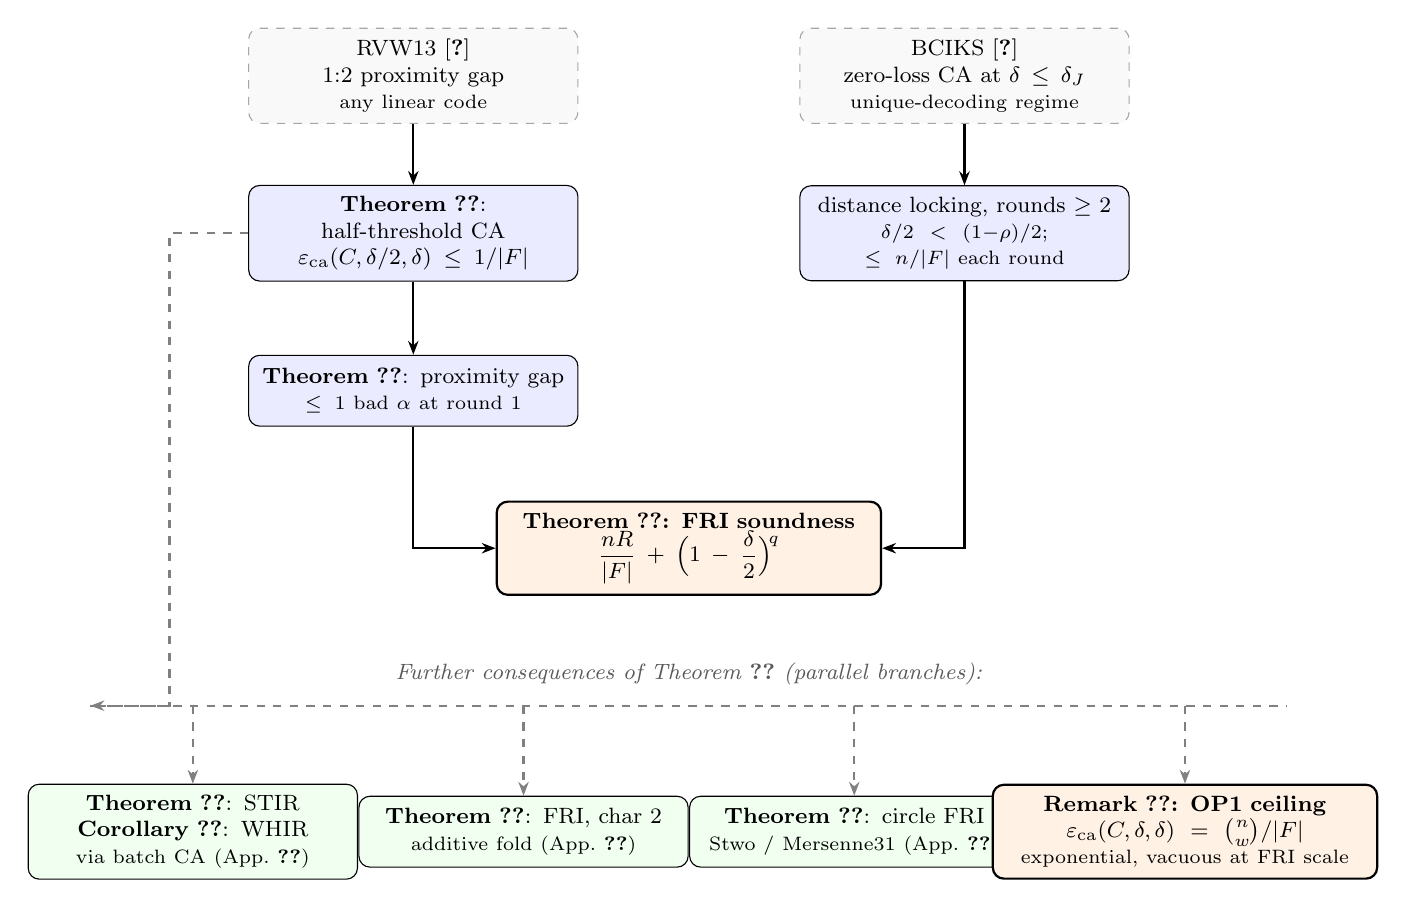
\begin{tikzpicture}[
  box/.style    ={draw, rounded corners, text width=3.9cm, minimum height=0.9cm,
                  align=center, font=\footnotesize, inner sep=4pt},
  mainbox/.style  ={box, fill=blue!8},
  extbox/.style   ={box, fill=green!6},
  resultbox/.style={box, fill=orange!10, thick, text width=4.6cm},
  inputbox/.style ={box, draw=gray!70, fill=gray!5, dashed},
  hub/.style      ={draw=gray!50, dashed, rounded corners, inner sep=10pt},
  arr/.style      ={-{Stealth[length=5pt]}, thick}
]
%%% ---- MAINLINE (top half) ---------------------------------------------
% Row A: inputs
\node[inputbox] (rvw)   at (-3.5, 0)    {RVW13~\cite{RVW}\\$1{:}2$ proximity gap\\{\scriptsize any linear code}};
\node[inputbox] (bciks) at ( 3.5, 0)    {BCIKS~\cite{BCIKS}\\zero-loss CA at $\delta\leq\delta_J$\\{\scriptsize unique-decoding regime}};

% Row B: our CA + distance lock
\node[mainbox]  (ca)    at (-3.5,-2.0)  {\textbf{Theorem~\ref{thm:ca-halved}}: half-threshold CA\\$\varepsilon_{\mathrm{ca}}(C,\delta/2,\delta)\leq 1/|F|$};
\node[mainbox]  (lock)  at ( 3.5,-2.0)  {distance locking, rounds $\geq 2$\\{\scriptsize $\delta/2<(1{-}\rho)/2$;\ $\leq n/|F|$ each round}};

% Row C: proximity gap (round 1)
\node[mainbox]  (pg)    at (-3.5,-4.0)  {\textbf{Theorem~\ref{thm:proximity-gap}}: proximity gap\\{\scriptsize $\leq 1$ bad $\alpha$ at round 1}};

% Row D: result
\node[resultbox](fri)   at ( 0.0,-6.0)  {\textbf{Theorem~\ref{thm:fri-full}: FRI soundness}\\$\dfrac{nR}{|F|}+\Bigl(1-\dfrac{\delta}{2}\Bigr)^{\!q}$};

% Mainline arrows (no crossings)
\draw[arr] (rvw)   -- (ca);
\draw[arr] (bciks) -- (lock);
\draw[arr] (ca)    -- (pg);
\draw[arr] (pg.south) |- (fri.west);
\draw[arr] (lock.south) |- (fri.east);

%%% ---- BRANCHING HUB (bottom half) -------------------------------------
% A horizontal bus at y = -8.0 (well below FRI at y=-6) collects from ca via
% a single rightward+downward route, then splits to four boxes below it.
\coordinate (busL) at (-7.6,-8.0);
\coordinate (busR) at ( 7.6,-8.0);
% Hub label sits just above the bus
\node[font=\footnotesize\itshape, text=gray!70!black]
      (huble) at (0,-7.6) {\,Further consequences of Theorem~\ref{thm:ca-halved} (parallel branches):\,};

% Row E: extensions + OP1, four boxes side by side
\node[extbox]    (stir) at (-6.3,-9.6) {\textbf{Theorem~\ref{thm:stir-full}}: STIR\\\textbf{Corollary~\ref{cor:whir}}: WHIR\\{\scriptsize via batch CA (App.~\ref{app:stir})}};
\node[extbox]    (fri2) at (-2.1,-9.6) {\textbf{Theorem~\ref{thm:fri-char2}}: FRI, char~2\\{\scriptsize additive fold (App.~\ref{app:char2})}};
\node[extbox]    (fric) at ( 2.1,-9.6) {\textbf{Theorem~\ref{thm:fri-circle}}: circle FRI\\{\scriptsize Stwo / Mersenne31 (App.~\ref{app:circle})}};
\node[resultbox] (op1)  at ( 6.3,-9.6) {\textbf{Remark~\ref{rem:barrier}: OP1 ceiling}\\$\varepsilon_{\mathrm{ca}}(C,\delta,\delta)=\binom{n}{w}/|F|$\\{\scriptsize exponential, vacuous at FRI scale}};

% Bus-style routing: single dashed line from ca's left side going around to
% the bus, then short straight drops to each box. Routed via the left margin
% (x = -6.0) to stay clear of pg and fri.
\draw[arr, dashed, gray]  (ca.west) -- ++(-1.0, 0) |- (busL);
\draw[dashed, gray, thick] (busL) -- (busR);
\draw[arr, dashed, gray]  (busL -| stir.north) -- (stir.north);
\draw[arr, dashed, gray]  (busL -| fri2.north) -- (fri2.north);
\draw[arr, dashed, gray]  (busL -| fric.north) -- (fric.north);
\draw[arr, dashed, gray]  (busL -| op1.north)  -- (op1.north);

\end{tikzpicture}
\end{adjustbox}
\caption{Proof map. \textbf{Top half} (mainline): RVW13 yields the half-threshold CA bound (Theorem~\ref{thm:ca-halved}), which composes with the FRI even/odd coupling to give the round-1 proximity gap (Theorem~\ref{thm:proximity-gap}); BCIKS supplies the round-$\geq 2$ distance lock (the structural observation $\delta/2<(1{-}\rho)/2$); the two combine into the FRI soundness theorem. \textbf{Bottom half} (parallel branches from the same CA bound): STIR/WHIR via batch CA; characteristic-$2$ FRI via additive coupling; circle FRI via the Stwo coupling; equal-threshold CA (the OP1 ceiling) showing the $\binom{n}{w}/|F|$ bound is vacuous at FRI scale, so the $2{\times}$ overhead is intrinsic to any CA-based proof. The list-size structural track (\S\ref{sec:list-size}) is independent of the soundness proof and is not shown.}
\label{fig:structure}
\end{figure}


%% ===================================================================
\section{Half-Threshold CA Bound}
\label{sec:ca}

\begin{theorem}[RVW13~\cite{RVW}; BCHKS~\cite{BCHKS}, Table~1, row~1]
\label{thm:ca-halved}
For any linear code $C$ over~$F$ with $|L| = n$:
$\varepsilon_{\mathrm{ca}}(C, \delta/2, \delta) \leq 1/|F|$.

Equivalently: for any $f_1, f_2 : L \to F$ with $\Delta_{\mathrm{joint}}((f_1, f_2),\, C \times C) > \delta$, at most one $\gamma \in F$ satisfies $\Delta(f_1 + \gamma f_2, C) \leq \delta/2$.
\end{theorem}

\noindent\textbf{Proof (due to~\cite{RVW}).} Two bad~$\gamma$'s give two linear equations in~$(f_1, f_2)$ on overlapping agreement sets. Solving for both components simultaneously yields a pair $(g_1, g_2) \in C \times C$ matching~$(f_1, f_2)$ on $\geq (1{-}\delta)n$ points, so joint distance $\leq \delta$ --- contradicting the premise.

\begin{proof}
Fix $f_1, f_2$ with $\Delta_{\mathrm{joint}} > \delta$. Call $\gamma$ ``bad'' if $\exists\, h_\gamma \in C$ with $\Delta(f_1 + \gamma f_2, h_\gamma) \leq \delta/2$; let $S_\gamma = \{x \in L : f_1(x) + \gamma f_2(x) = h_\gamma(x)\}$, so $|S_\gamma| \geq (1-\delta/2)n$.

Suppose $\gamma_1 \neq \gamma_2$ are both bad. By inclusion-exclusion:
$$|S_{\gamma_1} \cap S_{\gamma_2}| \;\geq\; 2(1-\delta/2)n - n \;=\; (1-\delta)n.$$

On $S_{\gamma_1} \cap S_{\gamma_2}$, the system $f_1 + \gamma_i f_2 = h_i$ ($i = 1, 2$) has the unique solution
$$g_1 := \frac{\gamma_2 h_1 - \gamma_1 h_2}{\gamma_2 - \gamma_1} \in C, \qquad g_2 := \frac{h_1 - h_2}{\gamma_1 - \gamma_2} \in C$$
(using linearity of~$C$). So $(f_1, f_2) = (g_1, g_2)$ on $S_{\gamma_1} \cap S_{\gamma_2}$, giving:
$$\Delta_{\mathrm{joint}}\bigl((f_1, f_2),\, C \times C\bigr) \;\leq\; \frac{|L \setminus (S_{\gamma_1} \cap S_{\gamma_2})|}{n} \;\leq\; \delta.$$
This contradicts $\Delta_{\mathrm{joint}} > \delta$. Hence at most $1$ bad~$\gamma$.
\end{proof}

\begin{remark}[Attribution and scope]
\label{rem:tighter}
Theorem~\ref{thm:ca-halved} is the classical $1{:}2$ proximity-gap inequality of Rothblum--Vadhan--Wigderson~\cite{RVW} (STOC 2013), formalized in BCHKS~\cite{BCHKS}, Table~1, as the row $[\text{RVW13}]{:}\; \gamma\text{ arbitrary},\; a \geq 2,\; \varepsilon^* = \gamma$. The proof uses only linearity of~$C$ (closure under $F$-linear combinations): no polynomial structure, no multiplicative structure on~$L$, no restriction on~$k$ or~$\delta$. It applies to any linear code over any finite field.

\emph{What is new in this paper} is not the CA bound, but (a)~its application \emph{above the Johnson radius} to obtain an unconditional FRI soundness theorem in the open zone $(\delta_J, 1{-}\rho)$, where no such theorem was previously available; (b)~the analytic equal-threshold CA bound $\varepsilon_{\mathrm{ca}} = \binom{n}{w}/|F|$ (Remark~\ref{rem:barrier}); and (c)~the tightness argument showing the $1{:}2$ ratio is optimal at FRI scale (Remark~\ref{rem:barrier}). The structural observation enabling~(a) is that $\delta/2 < (1{-}\rho)/2$ always, so after one round the protocol enters the unique-decoding regime where BCIKS~\cite{BCIKS} supplies the round-by-round gap.

The prior proximity-gap results of AHIV17~\cite{AHIV} ($\delta < \delta_V/4$), RZ18~\cite{RZ} ($\delta < \delta_V/3$), and BKS18~\cite{BKS} ($\delta$ above unique decoding) each proved successively stronger gap statements. The BKS18 FRI soundness proof~\cite{BKS} (Theorem~16, the one used by BCIKS~\cite{BCIKS}) splits on $\Delta(f_2, C)$ and bounds bad~$\alpha$'s in each case separately (\emph{Case~1/2}), yielding a 1:3 ratio ($\delta_{\mathrm{hd}} = \delta/3$), tight for that framework because the case bookkeeping gives $2\delta_{\mathrm{hd}} + \delta_{\mathrm{hd}} = 3\delta_{\mathrm{hd}} \leq \delta$ only when $\delta_{\mathrm{hd}} \leq \delta/3$. The direct proof above bypasses Case~1/2 entirely: it solves for \emph{both} $f_1$ and~$f_2$ simultaneously from two bad~$\gamma$'s, obtaining the \emph{joint} distance bound $\leq 2\delta_{\mathrm{hd}}$ in one step. This is $\leq \delta$ when $\delta_{\mathrm{hd}} \leq \delta/2$, improving the ratio from 1:3 to 1:2.

We state $nR/|F|$ (not $R/|F|$) in Theorem~\ref{thm:fri-full} to maintain a unified presentation with STIR (Theorem~\ref{thm:stir-full}), where the per-round count cannot be tightened below~$n$ in general.
\end{remark}


%% ===================================================================
\section{Equal-Threshold CA: Exact Bound and Tightness of the 1:2 Ratio}
\label{sec:barrier}

This section establishes the exact form of the equal-threshold CA bound (Theorem~\ref{thm:eq-threshold-upper}) and shows that it is tight up to lower-order terms (Proposition~\ref{prop:eq-threshold-tight}). The conclusion (Remark~\ref{rem:barrier}) is that the $\binom{n}{w}$ constant is exponential in the code length, vacuous at FRI scale; this is the formal statement behind the ``OP1 obstruction'' framing of \S\ref{sec:abf}.

\subsection{Upper bound at equal threshold}

\begin{theorem}[Equal-threshold CA upper bound]
\label{thm:eq-threshold-upper}
Let $C = \RS[F, L, k]$ with $|L| = n$, $w = n - k - 1$, $\delta = w/n$. For any $f_1, f_2 : L \to F$ satisfying $\Delta_{\mathrm{joint}}((f_1, f_2),\, C \times C) > \delta$:
$$\bigl|\{\gamma \in F : \Delta(f_1 + \gamma f_2,\, C) \leq \delta\}\bigr| \;\leq\; \binom{n}{w}.$$
Consequently $\varepsilon_{\mathrm{ca}}(C, \delta, \delta) \leq \binom{n}{w}/|F|$.
\end{theorem}

\begin{proof}
Let $\Gamma = \{\gamma \in F : \Delta(f_1 + \gamma f_2, C) \leq \delta\}$. For each $\gamma \in \Gamma$ there exists a witness codeword $c_\gamma \in C$ with $d(f_1 + \gamma f_2,\, c_\gamma) \leq \delta n = w$, so the agreement set has size $\geq n - w = k + 1$. Choose any $A_\gamma \subseteq L$ with $|A_\gamma| = k + 1$ on which $f_1 + \gamma f_2 = c_\gamma$, and define the assignment
$$\varphi : \Gamma \to \binom{L}{k+1}, \qquad \varphi(\gamma) = A_\gamma.$$

\noindent\emph{Claim: $\varphi$ is injective.} Suppose $\gamma \neq \gamma'$ in $\Gamma$ with $\varphi(\gamma) = \varphi(\gamma') = A$. On $A$ (size $k+1$):
$$f_1 + \gamma f_2 = c_\gamma, \qquad f_1 + \gamma' f_2 = c_{\gamma'}.$$
Subtracting and dividing by $\gamma - \gamma' \neq 0$ (allowed since $C$ is closed under $F$-linear combinations):
$$f_2 \bigr|_A \;=\; \tfrac{c_\gamma - c_{\gamma'}}{\gamma - \gamma'} \bigr|_A, \qquad g_2 := \tfrac{c_\gamma - c_{\gamma'}}{\gamma - \gamma'} \in C.$$
Likewise $f_1|_A = c_\gamma|_A - \gamma g_2|_A$, so setting $g_1 := c_\gamma - \gamma g_2 \in C$ gives $(f_1, f_2) = (g_1, g_2)$ on $A$. Hence the joint disagreement is at most $|L \setminus A| = n - (k+1) = w$, so
$$\Delta_{\mathrm{joint}}\bigl((f_1, f_2),\, C \times C\bigr) \;\leq\; \frac{w}{n} \;=\; \delta,$$
contradicting the hypothesis $\Delta_{\mathrm{joint}} > \delta$. Therefore $\varphi$ is injective and $|\Gamma| \leq \binom{n}{k+1} = \binom{n}{w}$.
\end{proof}

\begin{remark}[Scope of Theorem~\ref{thm:eq-threshold-upper}]
\label{rem:eq-threshold-scope}
The bound holds (i)~for \emph{all} $(f_1, f_2)$ with $\Delta_{\mathrm{joint}} > \delta$ — not just generic ones; (ii)~over \emph{any} field~$F$, including small fields where $|F| \leq \binom{n}{w}$ (in which case the bound $\binom{n}{w}/|F| \geq 1$ is trivial); (iii)~at the specific weight $w = n - k - 1$ (the largest~$w$ with $\delta n < n - k$, i.e., one below the covering radius). For $w' \leq w$ (smaller decoding ball, same code): the same $(k{+}1)$-subset injection yields $|\Gamma| \leq \binom{n}{k+1} = \binom{n}{w}$, since the agreement set still has size $\geq n - w' \geq k + 1$. Tighter bounds at $w' < w$ require a different argument (e.g., injection into $(n{-}w')$-subsets together with intersection constraints).
\end{remark}

\subsection{Tightness}

\begin{proposition}[Equal-threshold CA lower bound, large field]
\label{prop:eq-threshold-tight}
With notation as in Theorem~\ref{thm:eq-threshold-upper}, for every field $F$ with $|F| > \binom{n}{w}^2$ there exist $f_1, f_2: L \to F$ with $\Delta_{\mathrm{joint}}((f_1, f_2),\, C \times C) > \delta$ and
$$\bigl|\{\gamma \in F : \Delta(f_1 + \gamma f_2,\, C) \leq \delta\}\bigr| \;=\; \binom{n}{w}.$$
\end{proposition}

\begin{proof}
For each $(k+1)$-subset $A \subset L$, encode $A$-consistency of $f_1 + \gamma f_2$ as a single linear equation in~$\gamma$. Fix $A$ and let $\pi_A : F^L \to F$ be the linear functional defined by: $\pi_A(f) :=$ (value of the unique degree-${<}k$ Lagrange interpolant of $f|_{A_0}$ at the remaining point of~$A$) $-$ $f$ at that point, where $A_0$ is any fixed $k$-subset of $A$ (the choice of~$A_0$ does not affect the kernel). Then $f$ agrees with some codeword of $C$ on all of $A$ iff $\pi_A(f) = 0$. Set
$$a_A := \pi_A(f_1) \in F, \qquad b_A := \pi_A(f_2) \in F.$$
By linearity of $\pi_A$: $\pi_A(f_1 + \gamma f_2) = a_A + \gamma \cdot b_A$. Hence $f_1 + \gamma f_2$ is $A$-consistent iff
\begin{equation}
\label{eq:gamma-A}
a_A + \gamma \cdot b_A \;=\; 0.
\end{equation}
For $b_A \neq 0$, equation~\eqref{eq:gamma-A} has the unique solution $\gamma_A = -a_A/b_A \in F$. As $A$ ranges over the $\binom{n}{k+1} = \binom{n}{w}$ choices, the values $\{\gamma_A\}_A$ exhaust all candidate decodable~$\gamma$'s by Theorem~\ref{thm:eq-threshold-upper}'s injection (when each agreement set is exactly $(k{+}1)$-sized, the injection becomes a bijection onto its image).

\emph{Construction.} Fix $f_2 \in F^L$ such that $b_A(f_2) \neq 0$ for every $A \in \binom{L}{k+1}$; the bad set $\{f : \pi_A(f) = 0\}$ is a single proper hyperplane in $F^L$ for each~$A$, contributing $|F|^{n-1}/|F|^n = 1/|F|$ measure, so the union of $\binom{n}{w}$ such hyperplanes leaves at least $|F|^n (1 - \binom{n}{w}/|F|) > 0$ valid $f_2$ when $|F| > \binom{n}{w}$. Pick $f_1 \in F^L$ uniformly at random. For $A \neq A'$: the equation $\gamma_A = \gamma_{A'}$ becomes
$$a_A b_{A'} - a_{A'} b_A \;=\; 0 \;\;\Longleftrightarrow\;\; b_{A'} \cdot \pi_A(f_1) - b_A \cdot \pi_{A'}(f_1) \;=\; 0,$$
a single linear constraint on $f_1$. Since $\pi_A$ and $\pi_{A'}$ are non-proportional functionals (their kernels differ — they encode interpolation residuals on different $(k{+}1)$-subsets), the linear combination $b_{A'} \pi_A - b_A \pi_{A'}$ is a nonzero functional on $F^L$, hence vanishes on a hyperplane of measure $1/|F|$. By union bound over $\binom{\binom{n}{w}}{2} \leq \binom{n}{w}^2/2$ pairs:
$$\Pr_{f_1}[\text{some } \gamma_A = \gamma_{A'}] \;\leq\; \frac{\binom{n}{w}^2}{2 \, |F|} \;<\; 1$$
provided $|F| > \binom{n}{w}^2/2$. The hypothesis $|F| > \binom{n}{w}^2$ suffices, giving an $f_1$ with all $\binom{n}{w}$ values $\gamma_A$ pairwise distinct in~$F$. By construction each $\gamma_A$ is decodable (witnessed by codeword agreement on the $(k{+}1)$-subset~$A$), so $|\Gamma| \geq \binom{n}{w}$. Combined with the upper bound (Theorem~\ref{thm:eq-threshold-upper}), $|\Gamma| = \binom{n}{w}$.

\emph{Joint-distance check.} We must verify $\Delta_{\mathrm{joint}}((f_1, f_2), C \times C) > \delta$. If $\Delta_{\mathrm{joint}} \leq \delta$, then there exists a codeword pair $(g_1, g_2) \in C \times C$ with $|\{x : (f_1(x), f_2(x)) \neq (g_1(x), g_2(x))\}| \leq \delta n$. For \emph{any} $\gamma \in F$: $f_1 + \gamma f_2$ agrees with $g_1 + \gamma g_2 \in C$ on $\geq (1 - \delta) n$ points, so every $\gamma \in F$ would be decodable, giving $|\Gamma| = |F|$. But the construction gives $|\Gamma| = \binom{n}{w} < |F|$ (since $|F| > \binom{n}{w}^2 \geq \binom{n}{w}$). Therefore $\Delta_{\mathrm{joint}} > \delta$.
\end{proof}

\begin{corollary}[Asymptotic equality]
\label{cor:eq-threshold-equality}
For $|F|$ large enough (specifically $|F| > \binom{n}{w}^2$):
$$\varepsilon_{\mathrm{ca}}(C, \delta, \delta) \;=\; \frac{\binom{n}{w}}{|F|}.$$
\end{corollary}

\subsection{Computational verification}

The exact bound is verified for small parameters where exhaustive enumeration is feasible.

\begin{remark}[Empirical confirmation]
\label{rem:eq-threshold-empirical}
For $\mathrm{RS}[6, 3]$ over $\FF_q$, $q \in \{7, 13, 19, \ldots, 163\}$: the empirical maximum (over all tested $(f_1, f_2)$) of the number of $\delta$-close~$\gamma$'s equals $\min(q, \binom{6}{2}) = \min(q, 15)$ exactly. For $\mathrm{RS}[8, 4]$ over $q \in \{17, \ldots, 281\}$: $\min(q, \binom{8}{3}) = \min(q, 56)$, also exactly. See Note~\cite{Note0089}; scripts \texttt{op1\_scaling.py} and \texttt{op1\_scaling\_n8.py} in~\cite{CompanionRepo}.
\end{remark}

\subsection{Why the 1:2 ratio is optimal at FRI scale}

\begin{remark}[Why the 1:2 ratio is tight]
\label{rem:barrier}
\emph{Algebraic ceiling.} The proof of Theorem~\ref{thm:ca-halved} shows: two bad~$\gamma$'s at conclusion threshold~$\delta_{\mathrm{hd}}$ produce a joint pair $(g_1, g_2) \in C \times C$ matching $(f_1, f_2)$ on $\geq (1 - 2\delta_{\mathrm{hd}})n$ points, giving $\Delta_{\mathrm{joint}} \leq 2\delta_{\mathrm{hd}}$. For this to contradict $\Delta_{\mathrm{joint}} > \delta$: need $2\delta_{\mathrm{hd}} \leq \delta$, i.e., $\delta_{\mathrm{hd}} \leq \delta/2$. The bound $\delta_{\mathrm{hd}} = \delta/2$ is therefore \emph{optimal} for any argument that extracts a joint codeword pair from two bad random-linear-combination values.

\emph{Why pushing to equal threshold is vacuous.} By Corollary~\ref{cor:eq-threshold-equality}, the equal-threshold bound is exactly $\binom{n}{w}/|F|$ for sufficiently large fields. The constant $\binom{n}{w}$ grows as $2^{nH(\delta)}$ (Stirling). At FRI-relevant code lengths ($n \geq 2^{10}$, $|F| {\sim} 2^{31}$): $\binom{n}{w} \gg |F|$, so $\binom{n}{w}/|F| \gg 1$ and the equal-threshold bound is vacuous. The $2\times$ query overhead is intrinsic at FRI scale, even though $\varepsilon_{\mathrm{ca}}(C,\delta,\delta)$ is technically $O(1)/|F|$ for any fixed~$n$.

\emph{Half-threshold is tight.} At $\delta_{\mathrm{hd}} = \delta/2$, $\max_\gamma \leq 1$ in all tested cases~\cite{CompanionRepo}, matching the $\leq 1$ bound of Theorem~\ref{thm:ca-halved}. The constant~$2$ in the half-threshold bound is \emph{independent of~$n$}, in sharp contrast to the $\binom{n}{w}$ constant at equal threshold.

\emph{Comparison with the BKS18 1:3 ratio.} The BKS18~\cite{BKS} \emph{Case~1/2} approach (split on $\Delta(f_2, C)$, bound each case separately) achieves ratio~1:3 with \emph{zero} proximity loss at $\delta_{\mathrm{hd}} < \delta/3$. The RVW13~\cite{RVW} 2$\times$2-solve argument of Theorem~\ref{thm:ca-halved} trades zero loss for a better ratio (1:2 with loss~$\delta_{\mathrm{hd}}$); the 1:2 ratio has been folklore in the proximity-gap community since 2013.
\end{remark}


%% ===================================================================
\section{FRI Coupling and Proximity Gap}
\label{sec:fri}

\begin{lemma}[FRI Coupling, even $k$]
\label{lem:fri-coupling}
For even~$k$ and any $f: L \to F$:
$\Delta(f, \RS_k) \leq \Delta((f_{\mathrm{even}}, f_{\mathrm{odd}}), \RS_{k/2}^{=2})$.
\end{lemma}

\begin{proof}
By Remark~\ref{rem:k-parity}: $g \mapsto (g_{\mathrm{even}}, g_{\mathrm{odd}})$ is an isomorphism $\RS_k \to \RS_{k/2}^{=2}$. For any $g \in \RS_k$ and $y \in L'$ let $c_y := |\{x \in \{\sqrt{y}, -\sqrt{y}\} : f(x) \neq g(x)\}| \in \{0, 1, 2\}$ denote the number of base-level errors in the fibre over~$y$. If $f_{\mathrm{even}}(y) = g_{\mathrm{even}}(y)$ and $f_{\mathrm{odd}}(y) = g_{\mathrm{odd}}(y)$, then $f(\pm\sqrt{y}) = g(\pm\sqrt{y})$, so every joint-error position $y$ contributes $c_y \geq 1$ error on~$L$ and at most~$2$. Let $E = |\{y \in L' : c_y \geq 1\}|$ denote the number of joint-error positions. Then $\Delta(f,g) = \sum_y c_y / n \leq 2E / n = E / |L'| = \Delta_{\mathrm{joint}}$, where the cancellation uses $n = 2|L'|$. Taking $\min_g$ (using the isomorphism, the min over $\RS_{k/2}^{=2}$ equals the min over $\RS_k$):
$\Delta(f, \RS_k) \leq \Delta_{\mathrm{joint}}$.
\end{proof}

\begin{theorem}[Half-Threshold Proximity Gap]
\label{thm:proximity-gap}
For even~$k$, $\delta_J < \delta < 1{-}\rho$, and $\Delta(f, \RS_k) > \delta$:
$$|\{\alpha \in F : \Delta(f_{\mathrm{even}} + \alpha f_{\mathrm{odd}}, \RS_{k/2}) \leq \delta/2\}| \leq 1.$$
\end{theorem}

\begin{proof}
By Lemma~\ref{lem:fri-coupling}: $\Delta((f_{\mathrm{even}}, f_{\mathrm{odd}}), \RS_{k/2}^{=2}) \geq \Delta(f, \RS_k) > \delta$. The isomorphism $\RS_k \xrightarrow{\sim} \RS_{k/2}^{=2}$ (Remark~\ref{rem:k-parity}) gives $\RS_{k/2}^{=2} = \RS_{k/2} \times \RS_{k/2}$, so $\Delta_{\mathrm{joint}}((f_{\mathrm{even}}, f_{\mathrm{odd}}), \RS_{k/2} \times \RS_{k/2}) > \delta$. Apply Theorem~\ref{thm:ca-halved} to $(f_1, f_2) = (f_{\mathrm{even}}, f_{\mathrm{odd}})$ on $C = \RS_{k/2}$ over~$L'$, with $\alpha$ drawn from the challenge field~$F$ (typically an extension of the field containing~$L'$; see Remark~\ref{rem:extension}): at most $1$~value of~$\alpha \in F$ has $\Delta(f_{\mathrm{even}} + \alpha f_{\mathrm{odd}}, \RS_{k/2}) \leq \delta/2$.
\end{proof}


%% ===================================================================
\section{FRI Soundness}
\label{sec:soundness}

\begin{definition}[Standard FRI query model]
\label{def:query-model}
The verifier samples $q$ base-level points $z_1, \ldots, z_q \in L$ \textbf{i.i.d.\ uniform with replacement}; for each $z_j$ it queries the folding-tree path $z_j \to \pi_1(z_j) \to \pi_2(z_j) \to \cdots \to \pi_R(z_j)$, where $\pi_i: L \to L^{(i)}$ is the iterated squaring map, and at every round $i = 1, \ldots, R$ checks the consistency relation $f^{(i)}(\pi_i(z_j)) = f^{(i-1)}_{\mathrm{even}}(\pi_i(z_j)) + \alpha_i \cdot f^{(i-1)}_{\mathrm{odd}}(\pi_i(z_j))$. (Equivalent statements for additive folding (App.~\ref{app:char2}) and circle folding (App.~\ref{app:circle}) replace $\pi_i$ with the corresponding round-$i$ projection.)
\end{definition}

\begin{remark}[Implementation models: with-replacement vs.\ without-replacement]
\label{rem:query-model-impl}
This paper's bounds are stated for the i.i.d.\ with-replacement model (Definition~\ref{def:query-model}), which is standard in the FRI/STIR/WHIR analyses~\cite{BBHR,BCIKS,STIR,WHIR}. Deployed implementations typically draw $q$ \emph{distinct} base-level indices via Fiat--Shamir hashing (without replacement, or with domain separation that makes collisions cryptographically negligible). The without-replacement miss probability $\binom{|L| - |\pi_i^{-1}(D_i)|}{q}/\binom{|L|}{q}$ is bounded above by $(1-\tau)^q$ for the same $\tau = |D_i|/|L^{(i)}|$ (negative association of without-replacement indicators), so the bounds in Theorems~\ref{thm:fri-full}, \ref{thm:stir-full}, \ref{thm:whir-full} apply unchanged to deployed protocols.
\end{remark}

\begin{lemma}[Catch probability under i.i.d.\ base sampling]
\label{lem:catch-prob}
Under Definition~\ref{def:query-model}, fix any round~$i$ and any deviation set $D_i \subseteq L^{(i)}$ with $|D_i|/|L^{(i)}| \geq \tau$. Then
$$\Pr_{z_1, \ldots, z_q \stackrel{\textup{i.i.d.}}{\sim} L}\bigl[\,\pi_i(z_j) \notin D_i \text{ for all } j = 1, \ldots, q\,\bigr] \;\leq\; (1 - \tau)^q.$$
\end{lemma}

\begin{proof}
Let $X_j := \mathbf{1}\{\pi_i(z_j) \in D_i\}$. The map $\pi_i: L \to L^{(i)}$ is $2^i$-to-$1$ (a composition of $i$ squarings, each $2$-to-$1$ on the relevant subgroup), so $|\pi_i^{-1}(D_i)| = 2^i \cdot |D_i|$ and
$$\Pr_{z_j {\sim} L}[X_j = 1] \;=\; \frac{2^i \cdot |D_i|}{2^i \cdot |L^{(i)}|} \;=\; \frac{|D_i|}{|L^{(i)}|} \;\geq\; \tau.$$
The variables $X_1, \ldots, X_q$ are i.i.d.\ Bernoulli with parameter $\geq \tau$ because $z_1, \ldots, z_q$ are i.i.d.\ and each $X_j = h(z_j)$ for the deterministic function $h(z) = \mathbf{1}\{\pi_i(z) \in D_i\}$.  What matters is independence of the \emph{base-level} samples $z_j$, not of the \emph{induced} samples $\pi_i(z_j)$: the latter can collide (and are guaranteed to do so by pigeonhole in late rounds, when $|L^{(i)}| \leq q$), but the Bernoulli parameters $\Pr[X_j = 1]$ are identical across $j$, and the joint distribution factors as a product of Bernoullis regardless of induced collisions. Therefore
$$\Pr[X_1 = \cdots = X_q = 0] \;=\; \prod_{j=1}^q \Pr[X_j = 0] \;\leq\; (1 - \tau)^q. \qedhere$$
\end{proof}

\begin{theorem}[FRI Soundness Above Johnson]
\label{thm:fri-full}
For $\RS[F, L, k]$ with $\mathrm{char}(F) \neq 2$, $k = 2^m$, $L$ closed under negation, $\delta_J < \delta < 1{-}\rho$, and $\Delta(f^{(0)}, \RS_k) > \delta$: FRI with $R = m$ rounds and $q$ queries per round satisfies
$$\Pr[\textup{FRI accepts}] \leq \frac{nR}{|F|} + (1 - \delta/2)^q.$$
\end{theorem}

\begin{proof}
We partition all adaptive prover strategies into two cases according to whether the committed oracles match the honest fold. The prover sees $\alpha_i$ before committing $f^{(i)}$; the analysis below covers every such adaptive strategy.

\textbf{Strategy A: the prover commits the honest fold at every round.} In this case, $f^{(i)}$ is the function $f^{(i-1)}_{\mathrm{even}} + \alpha_i \cdot f^{(i-1)}_{\mathrm{odd}}$ (determined by $f^{(0)}$ and $\alpha_1, \ldots, \alpha_i$). No adaptive freedom remains: the prover's only choice was to fold honestly, and the resulting $f^{(R)}$ is a \emph{fixed} function of $f^{(0)}$ and $(\alpha_1, \ldots, \alpha_R)$.

For any fixed evaluation point $y \in L^{(R)}$, $f^{(R)}(y)$ is \emph{multilinear} in $(\alpha_1, \ldots, \alpha_R)$ --- individual degree~$\leq 1$ in each $\alpha_i$ (one round introduces each variable, each via the linear even/odd combination $f^{(i-1)}_{\mathrm{even}} + \alpha_i \cdot f^{(i-1)}_{\mathrm{odd}}$).  Consequently, every syndrome $s_j(f^{(R)}) = \sum_y c_y \cdot f^{(R)}(y)$ is multilinear in $(\alpha_1, \ldots, \alpha_R)$.

\emph{Some syndrome is nonzero as a polynomial.} Suppose all syndromes vanished identically (as polynomials in $\alpha_1, \ldots, \alpha_R$). Then $f^{(R)} \in \RS_{k/2^R}$ for \emph{every} choice of $(\alpha_1, \ldots, \alpha_R) \in F^R$. We extract $f^{(0)} \in \RS_k$ from this universal hypothesis as a polynomial-identity argument (\emph{not} a protocol-level reconstruction; FRI does not expose intermediate $f^{(i-1)}_{\mathrm{even}}, f^{(i-1)}_{\mathrm{odd}}$, and an attacker cannot reconstruct $f^{(0)}$ from~$f^{(R)}$ at runtime). For each round $i = R, R{-}1, \ldots, 1$: by the multilinearity in $\alpha_i$, evaluating at $\alpha_i = 0$ yields $f^{(i-1)}_{\mathrm{even}} \in \RS_{k/2^i}$, and the difference at $\alpha_i = 1$ minus $\alpha_i = 0$ yields $f^{(i-1)}_{\mathrm{odd}} \in \RS_{k/2^i}$ (each as a function of $\alpha_1, \ldots, \alpha_{i-1}$, with $|F| \geq 2$ ensuring two distinct evaluation points). The isomorphism of Remark~\ref{rem:k-parity} --- which requires $k/2^{i-1}$ even, guaranteed by $k = 2^m$ --- then gives $f^{(i-1)} \in \RS_{k/2^{i-1}}$. Iterating to $i=1$ yields $f^{(0)} \in \RS_k$, contradicting the hypothesis. Hence there exists a syndrome~$s_j$ that is a nonzero multilinear polynomial.

Since $s_j$ is multilinear in $\alpha_1, \ldots, \alpha_R$ (individual degree $\leq 1$ in each variable), the DeMillo--Lipton--Schwartz--Zippel lemma in the individual-degree form (a nonzero polynomial with individual degree $\leq d_i$ in variable $i$ vanishes on a uniformly random point with probability $\leq \sum_i d_i / |F|$) gives
$$\Pr_{\alpha_1, \ldots, \alpha_R \stackrel{\textup{i.i.d.}}{\sim} F}[s_j(f^{(R)}) = 0] \;\leq\; R/|F|.$$
A fortiori, $\Pr[f^{(R)} \in \RS_{k/2^R}] \leq R/|F|$.

\textbf{Strategy B: any prover strategy with at least one deviation.}
We give a single round-by-round argument that applies uniformly to every adaptive prover, regardless of how many rounds it deviates at and whether its commits are codewords or not.  This replaces an earlier exposition that case-split on single-vs-multi deviation and on a ``lucky/unlucky'' challenge dichotomy; the case split conflated the prover's commit chain with the honest-fold chain.  The argument below tracks the honest-fold chain explicitly, which is the standard round-by-round (RBR) FRI soundness framework~\cite{BBHR,BCIKS,BGKTTW} and is also the form taken by Theorem~\ref{thm:fri-rbr} in \S\ref{subsec:rbr}.

\emph{Honest-fold reference sequence.}
Define
\[
\hat f^{(0)} := f^{(0)}, \qquad
\hat f^{(i)}(y) := \hat f^{(i-1)}_{\mathrm{even}}(y) + \alpha_i \cdot \hat f^{(i-1)}_{\mathrm{odd}}(y) \quad (y \in L^{(i)}).
\]
This is a deterministic function of $f^{(0)}$ and the verifier's challenges $(\alpha_1, \ldots, \alpha_R)$; in particular $\hat f^{(i)}$ does \emph{not} depend on the prover's subsequent commits $f^{(1)}, \ldots, f^{(R)}$.

\emph{Step 1 --- Bad-challenge bound: $\leq nR/|F|$.}
By induction on~$i$, we bound the probability that some $\hat f^{(i)}$ becomes $(\delta/2)$-close to $\RS_{k/2^i}$:
\begin{itemize}[nosep]
\item \emph{Round 1.} $\Delta(\hat f^{(0)}, \RS_k) = \Delta(f^{(0)}, \RS_k) > \delta$.  By Theorem~\ref{thm:proximity-gap}, at most $1$ value of $\alpha_1$ makes $\Delta(\hat f^{(1)}, \RS_{k/2}) \leq \delta/2$.  Probability~$\leq 1/|F|$.
\item \emph{Rounds $i = 2, \ldots, R$.}  Inductively assume $\Delta(\hat f^{(i-1)}, \RS_{k/2^{i-1}}) > \delta/2$.  Since $\delta < 1{-}\rho$ we have $\delta/2 < (1{-}\rho)/2 \leq \delta_J$, so the threshold $\gamma = \delta/2$ lies in the unique-decoding regime.  By Lemma~\ref{lem:fri-coupling}, $\Delta_{\mathrm{joint}}((\hat f^{(i-1)}_{\mathrm{even}}, \hat f^{(i-1)}_{\mathrm{odd}}), \RS_{k/2^i}^{=2}) > \delta/2$, and the BCIKS proximity gap~\cite{BCIKS} (Theorem~1.2, Eq.~(1.1)) at threshold~$\gamma = \delta/2$ gives: at most $n$ values of $\alpha_i$ make $\Delta(\hat f^{(i)}, \RS_{k/2^i}) \leq \delta/2$.  Probability $\leq n/|F|$.
\end{itemize}
Union over $R$ rounds: $\Pr[\exists i: \Delta(\hat f^{(i)}, \RS_{k/2^i}) \leq \delta/2] \leq 1/|F| + (R{-}1)n/|F| \leq nR/|F|$.

\emph{Step 2 --- Catch-probability bound: $\leq (1-\delta/2)^q$.}
Condition on the good event from Step~1: $\Delta(\hat f^{(i)}, \RS_{k/2^i}) > \delta/2$ for every~$i$.

If the prover commits $f^{(i)} = \mathrm{fold}(f^{(i-1)}, \alpha_i)$ at every round, then $f^{(i)} = \hat f^{(i)}$ at every round (induction on $i$ from the common base $f^{(0)} = \hat f^{(0)}$), so $\Delta(f^{(R)}, \RS_{k/2^R}) > \delta/2 > 0$, $f^{(R)} \notin \RS_{k/2^R}$, and the final check rejects.  The verifier therefore accepts only if the prover commits at least one $f^{(i)}$ that disagrees with the fold of its own previous commit (the verifier-checkable notion of deviation), in such a way that the resulting chain reaches $f^{(R)} \in \RS_{k/2^R}$.

Define the round-$i$ \emph{deviation set} (relative to the prover's own previous commit $f^{(i-1)}$, since this is what the verifier's consistency check examines):
\[
B_i := \{y \in L^{(i)} : f^{(i)}(y) \neq f^{(i-1)}_{\mathrm{even}}(y) + \alpha_i \cdot f^{(i-1)}_{\mathrm{odd}}(y)\}, \qquad \beta_i := |B_i|/|L^{(i)}|.
\]
A query $z_j \in L$ ``catches'' the prover at round~$i$ iff $\pi_i(z_j) \in B_i$, so the verifier rejects $z_j$ iff $z_j \in T := \bigcup_{i=1}^R \pi_i^{-1}(B_i) \subseteq L$.

\emph{Path-consistency lemma.}  We use the standard FRI catch lemma~\cite[Lemma~4.1, \S6]{BBHR}, \cite[Lemma~8.2]{BCIKS} (also stated as Theorem~3.3 of~\cite{BCIKS} with explicit constants) in the following form: under the conditions $f^{(R)} \in \RS_{k/2^R}$ and $\Delta(\hat f^{(R)}, \RS_{k/2^R}) > \delta/2$, the merged catching set $T$ has relative measure at the base level satisfying $|T|/|L| \geq \delta/2$.  The proof in~\cite{BBHR,BCIKS} goes via a path-coverage argument: every level-$R$ point at which $f^{(R)}$ disagrees with $\hat f^{(R)}$ admits a level-$j$ ancestor on the fold tree that lies in $B_j$ for some $j \in \{1, \ldots, R\}$; counting paths through level-$R$ disagreements gives the $\delta/2$ lower bound on $|T|/|L|$.  We invoke the lemma as a black box; see the cited references for the detailed coverage argument.

By Lemma~\ref{lem:catch-prob} applied to $T$ with $\tau = \delta/2$: the probability that all $q$ i.i.d.\ base-level queries miss $T$ is at most $(1-\delta/2)^q$.

\emph{Combining Steps~1 and~2.}
\[
\Pr[\text{Strategy B succeeds}] \;\leq\; \frac{nR}{|F|} + (1 - \delta/2)^q.
\]
This bound holds simultaneously for any number of deviation rounds (single or multi) and any commit pattern (codeword or non-codeword), since the honest-fold reference and the merged catching set are defined uniformly across all prover strategies.

\textbf{Combining Strategies A and B.}
Every adaptive prover either folds honestly at every round (Strategy~A) or deviates at some round (Strategy~B):
\[
\Pr[\text{accept}] \;\leq\; \max\!\Bigl(\tfrac{R}{|F|},\; \tfrac{nR}{|F|} + (1{-}\delta/2)^q\Bigr) \;\leq\; \tfrac{nR}{|F|} + (1{-}\delta/2)^q. \qedhere
\]
\end{proof}

\begin{remark}[Why $\delta/2$ does not compound across rounds]
\label{rem:no-compound}
A common concern: the reduced threshold $\delta/2$ could degrade further at each round (to $\delta/4$, $\delta/8$, \ldots), eventually making the consistency check trivial. This does \emph{not} happen. After round~$1$ reduces the effective distance from~$\delta$ to~$\delta/2$, this threshold sits strictly below the \emph{unique decoding radius} $(1{-}\rho)/2$ (since $\delta/2 < (1{-}\rho)/2$ for any $\delta < 1{-}\rho$). The BCIKS proximity gap~\cite{BCIKS} (Theorem~1.2, Eq.~(1.1)) at threshold $\gamma = \delta/2 < (1{-}\rho)/2$ bounds the number of bad challenges to $\leq n$ per round. The distance remains~$\delta/2$ (not $\delta/4$) because we invoke the equal-threshold proximity gap rather than re-applying the two-threshold Theorem~\ref{thm:ca-halved} iteratively. In short: Theorem~\ref{thm:ca-halved} enters the unique decoding regime at round~$1$; the BCIKS proximity gap~\cite{BCIKS} then \emph{locks} the distance at~$\delta/2$ for all subsequent rounds.
\end{remark}


%% ===================================================================
\section{List-Size Landscape and OP2}
\label{sec:list-size}

The results in this section are independent of the FRI soundness theorem (Theorem~\ref{thm:fri-full}), which uses only the half-threshold CA (Theorem~\ref{thm:ca-halved}) and classical list decoding. They address Open Problem~2 (\S\ref{sec:open}): can one show $M = 0$ on all RS-compatible flats? We give the first $p$-dependent moment bound on the list size (Theorem~\ref{thm:second-moment} for $c = 1$; Corollary~\ref{cor:moments-c} for general~$c$), prove the $M = 0$ conjecture is false at deployment code lengths (Proposition~\ref{prop:m2-obstruction}), and reduce the remaining gap to a worst-case-from-average problem.

\begin{remark}[$p$-independent list-size bounds]
\label{rem:list-bounds}
Classical bounds give $M \leq n^2/(t(t{-}1))$ for $k = 2$ (Fisher double-counting; see Sudan~\cite{Sudan97}, Guruswami--Sudan~\cite{GuruswamiSudan} for general list decoding) and $M \leq \sum_{i=0}^{k-2c}\binom{n}{i}$ for general~$k$ (Frankl--Wilson~\cite{FranklWilson} linear algebra method), where $c = n{-}k{-}w$ is the codimension excess. Both are independent of~$p$ and cannot capture the $p^{-\alpha}$ decay observed computationally~\cite{CompanionRepo}: for $\RS[16,8]$ at $c = 1$, $M_{\max}(p) \approx 4200 \cdot p^{-3/4}$ across $19$~primes from $p = 17$ to $131$.
\end{remark}

\subsection{Syndrome hyperplane structure and second moment}
\label{sec:poisson}

Classical $p$-independent bounds (Remark~\ref{rem:list-bounds}) cannot capture the $p^{-\alpha}$ decay observed computationally. The following results explain this decay via the hyperplane geometry of syndrome space and provide the first $p$-dependent moment bounds on the list size. The results hold for \emph{all}~$k$.

Fix $\RS[n,k]$ over $\FF_p$ with $p > n$, evaluation domain $L = \{\alpha_1, \ldots, \alpha_n\}$, and codimension excess $c = 1$ (error weight $w = n - k - 1$, syndrome dimension $D = n - k$). For each $w$-subset $E \subset [n]$, the syndrome equations $\sum_{i \in E} e_i \alpha_i^j = s_j$ ($j = k, \ldots, n{-}1$) form a $D \times w$ Vandermonde system. With $D = w + 1$, the compatibility condition is a single hyperplane $H_E = \{s \in \FF_p^D : \langle n_E, s \rangle = 0\}$, and $M(s) = |\{E \in \binom{[n]}{w} : s \in H_E\}|$.

\begin{lemma}[Error-locator normal]
\label{lem:locator-normal}
The normal vector of $H_E$ is the coefficient vector of the error-locator polynomial:
$$n_E = (\Lambda_{E,0}, \ldots, \Lambda_{E,D-1}), \qquad \Lambda_E(x) = \prod_{e \in E}(x - \alpha_e).$$
\end{lemma}

\begin{proof}
Since $\alpha_e$ is a root of $\Lambda_E$: $\sum_{\ell=0}^{w} \Lambda_{E,\ell}\, \alpha_e^{k+\ell} = \alpha_e^k \Lambda_E(\alpha_e) = 0$ for each $e \in E$. So the vector $(\Lambda_{E,0}, \ldots, \Lambda_{E,w})$ annihilates every column of the $D \times w$ Vandermonde submatrix~$V_E$. Since $V_E$ has rank~$w$ (distinct evaluation points, $p > n$), its left kernel is $1$-dimensional and spanned by~$n_E$.
\end{proof}

\begin{lemma}[Pairwise independence]
\label{lem:pairwise-indep}
For distinct $w$-subsets $E_1 \neq E_2$, the normals $n_{E_1}$ and $n_{E_2}$ are linearly independent over~$\FF_p$.
\end{lemma}

\begin{proof}
Both $\Lambda_{E_1}$ and $\Lambda_{E_2}$ are monic of degree~$w$. Monic polynomials of the same degree are proportional only if equal, requiring identical root sets: $E_1 = E_2$.
\end{proof}

\begin{theorem}[Exact second moment of the list size]
\label{thm:second-moment}
For $\RS[n,k]$ over $\FF_p$ with $p > n$ and $c = 1$, the list size $M$ over uniform $s \in \FF_p^D$ satisfies:
$$\EE[M] = \frac{\binom{n}{w}}{p}, \qquad \Var[M] = \EE[M]\!\left(1 - \frac{1}{p}\right).$$
\end{theorem}

\begin{proof}
Write $M = \sum_E \mathbf{1}_{s \in H_E}$. Each indicator has $\Pr[s \in H_E] = 1/p$. For $E_1 \neq E_2$: by Lemma~\ref{lem:pairwise-indep}, $H_{E_1} \cap H_{E_2}$ has codimension~$2$ in $\FF_p^D$, so $\Pr[s \in H_{E_1} \cap H_{E_2}] = 1/p^2 = \Pr[s \in H_{E_1}] \cdot \Pr[s \in H_{E_2}]$. The indicators are pairwise uncorrelated, giving $\Var[M] = \binom{n}{w} \cdot \tfrac{1}{p}(1 - \tfrac{1}{p})$.
\end{proof}

\begin{remark}[Implications for the list-size landscape]
\label{rem:poisson}
\hfill

\noindent\emph{(i) Near-Poisson concentration.} For large~$p$: $\Var[M] \approx \EE[M]$, matching the Poisson dispersion relation. This justifies the heuristic that $M$ concentrates around $\binom{n}{w}/p$ and is typically~$0$ once $p > \binom{n}{w}$. For $\RS[16,8]$ at $c = 1$: $\binom{16}{7} = 11440$, so $\EE[M] < 1$ for $p \geq 11441$. The power-law decay of $M_{\max}$ (see Remark~\ref{rem:list-bounds}) is substantially sharper than the first-moment prediction, suggesting algebraic structure beyond pairwise independence governs the worst case.

\noindent\emph{(ii) The $c = 1$ threshold and $c \geq 2$ generalization.} At $c = 1$ (near capacity, $w = n{-}k{-}1$) with rate $\rho = 1/2$: $\binom{n}{w} = \binom{n}{n/2-1} {\sim} 2^n/\sqrt{n}$, so $\EE[M] < 1$ requires $p > 2^n/\sqrt{n}$ --- far beyond any practical field once $n$ exceeds a few dozen. At the \emph{FRI-relevant} distance $\delta > \delta_J$ with codimension $c = n/2 - \lfloor\delta n\rfloor \gg 1$ (for $\rho = 1/2$, just above Johnson gives $c \approx 0.2n$): Theorem~\ref{thm:pairwise-c} and Corollary~\ref{cor:moments-c} establish $\EE[M] = \binom{n}{w}/p^c$ with pairwise independence for all pairs with $|E_1 \cap E_2| \leq w - c$, giving $\Var[M] \approx \EE[M]$ (Poisson dispersion). At current code lengths, $\EE[M] = \binom{n}{w}/p^c \leq 2^{-5.3n} \approx 0$.

\noindent\emph{(iii) Average vs.\ worst case.} By Markov: $\Pr_{s}[M \geq 1] \leq \binom{n}{w}/p$. However, \S\ref{sec:open}, item~2, asks for $M_{\max} = 0$ over \emph{all} syndromes (or all RS-compatible flats). The second-moment bound $\Var[M] \leq \EE[M]$ does not improve on Markov for this worst-case question. Bridging the average-to-worst-case gap requires exploiting the algebraic structure of the error-locator hyperplane arrangement beyond pairwise independence --- for example, showing that the $\binom{n}{w}$ hyperplanes, despite their number, avoid all RS-compatible flats when $p$ is sufficiently large relative to~$n$.
\end{remark}


\subsection{Generalization to codimension excess $c \geq 2$}
\label{sec:poisson-c2}

Theorem~\ref{thm:second-moment} treats codimension excess $c = 1$, where each $w$-subset~$E$ defines a single hyperplane $H_E$ in syndrome space. For general $c \geq 2$ (error weight $w = n-k-c$, syndrome dimension $D = n-k$), the compatibility condition is $s \in W_E := \mathrm{Im}(V_E)$, the column span of the $D \times w$ Vandermonde submatrix~$V_E$. Since $V_E$ has rank~$w$ (MDS, $p > n$), $W_E$ is a $w$-dimensional subspace of~$\FF_p^D$, equivalently a codimension-$c$ subspace. Its orthogonal complement $W_E^\perp$ has dimension~$c$ and is the left null space of~$V_E$. The following results extend the error-locator normal structure and pairwise independence to this regime. The case $c \geq 2$ is the \emph{FRI-relevant} regime: at rate $\rho = 1/2$ and distance $\delta \approx 0.3$, the codimension excess is $c = n/2 - \lfloor 0.3n\rfloor \approx 0.2n$.

\begin{lemma}[Generalized normal space]
\label{lem:locator-normal-c}
For codimension excess $c \geq 1$, the left null space of the $D \times w$ Vandermonde submatrix~$V_E$ has dimension~$c$ and is spanned by the coefficient vectors of
$$\Lambda_E(x) \cdot x^r, \qquad r = 0, 1, \ldots, c-1,$$
where $\Lambda_E(x) = \prod_{e \in E}(x - \alpha_e)$ is the error-locator polynomial.
\end{lemma}

\begin{proof}
Since $\alpha_e$ is a root of~$\Lambda_E$, the polynomial $\Lambda_E(x) \cdot x^r$ vanishes at every $\alpha_e$ for $e \in E$. Its coefficient vector (as a polynomial of degree $w + r < D = w + c$, embedded in $\FF_p^D$) therefore annihilates every column of~$V_E$. The $c$ polynomials $\{\Lambda_E \cdot x^r\}_{r=0}^{c-1}$ have degrees $w, w{+}1, \ldots, w{+}c{-}1$; since $\Lambda_E$ is monic of degree~$w$, these have leading terms $x^w, x^{w+1}, \ldots, x^{w+c-1}$, so they are linearly independent. The left null space of~$V_E$ has dimension $D - w = c$ (distinct evaluation points, $p > n$), and $c$ linearly independent vectors span it.
\end{proof}

\begin{theorem}[Pairwise independence at $c \geq 2$]
\label{thm:pairwise-c}
For distinct $w$-subsets $E_1 \neq E_2$ with $j = |E_1 \cap E_2| \leq w - c$: the $2c$ normal vectors from Lemma~\ref{lem:locator-normal-c} (i.e., the coefficient vectors of $\{\Lambda_{E_1} x^r, \Lambda_{E_2} x^r : 0 \leq r < c\}$) are linearly independent over~$\FF_p$. Consequently:
$$W_{E_1} \cap W_{E_2} \text{ has codimension } 2c, \qquad \Pr_s[s \in W_{E_1} \cap W_{E_2}] = \frac{1}{p^{2c}} = \Pr_s[s \in W_{E_1}] \cdot \Pr_s[s \in W_{E_2}].$$
The membership indicators $\mathbf{1}_{s \in W_{E_1}}$ and $\mathbf{1}_{s \in W_{E_2}}$ are pairwise uncorrelated for uniform~$s$.
\end{theorem}

\begin{proof}
Suppose $\sum_{r=0}^{c-1} \bigl(a_r \Lambda_{E_1}(x) x^r + b_r \Lambda_{E_2}(x) x^r\bigr) = 0$ as polynomials of degree $< D = w + c$. Set $P(x) = \sum a_r x^r$ and $Q(x) = \sum b_r x^r$ (both of degree $< c$). Then $\Lambda_{E_1} P + \Lambda_{E_2} Q = 0$.

Let $G = \gcd(\Lambda_{E_1}, \Lambda_{E_2}) = \Lambda_{E_1 \cap E_2}$ of degree~$j$, and write $\Lambda_{E_i} = G \cdot A_i$ where $\gcd(A_1, A_2) = 1$ and $\deg A_i = w - j$. Dividing by~$G$: $A_1 P = -A_2 Q$. Since $\gcd(A_1, A_2) = 1$, we need $A_1 \mid Q$. But $\deg A_1 = w - j \geq w - (w - c) = c > \deg Q$, so $Q = 0$, hence $P = 0$.

The $2c$ normals are linearly independent, so $W_{E_1}^\perp + W_{E_2}^\perp$ has dimension~$2c$. Since $\dim(W_{E_1}^\perp) = \dim(W_{E_2}^\perp) = c$, the intersection $W_{E_1} \cap W_{E_2}$ has codimension~$2c$, giving exact independence.
\end{proof}

\begin{remark}[Sharpness of the threshold $j \leq w - c$]
\label{rem:threshold-sharp}
The threshold is sharp. For $j > w - c$, set $\ell = j - (w-c) \geq 1$. In the notation of the proof above, $\deg A_i = w - j = c - \ell$. For any polynomial $R$ of degree $< \ell$, setting $Q = A_1 R$ (degree $< c$) and $P = -A_2 R$ (degree $< c$) gives $\Lambda_{E_1} P + \Lambda_{E_2} Q = G(-A_1 A_2 R + A_2 A_1 R) = 0$: a nontrivial relation among the $2c$ normals. The space of such relations has dimension $\ell = j - (w-c)$, so the rank drops from $2c$ to $2c - \ell$.

In particular, at $j = w - c + 1$ ($\ell = 1$): rank $= 2c - 1$, verified computationally for all tested pairs~\cite{CompanionRepo}.
\end{remark}

\begin{corollary}[Exact moments of the list size at $c \geq 2$]
\label{cor:moments-c}
For $\RS[n,k]$ over $\FF_p$ with $p > n$, codimension excess $c \geq 1$, and $w = n-k-c$, define $M = |\{E \in \binom{[n]}{w} : s \in W_E\}|$ for uniform $s \in \FF_p^D$. Then:
$$\EE[M] = \frac{\binom{n}{w}}{p^c}.$$
For the variance, decomposing by intersection size $j = |E_1 \cap E_2|$:
\begin{equation}
\label{eq:var-decomp}
\Var[M] = \underbrace{\sum_{j=0}^{w-c} \binom{n}{w} \binom{w}{j}\binom{n-w}{w-j} \cdot 0}_{\text{pairwise independent: } j \leq w-c} \;+\; \underbrace{\sum_{j=w-c+1}^{w} \binom{n}{w}\binom{w}{j}\binom{n-w}{w-j}\Bigl(\frac{1}{p^{2c-\ell(j)}} - \frac{1}{p^{2c}}\Bigr)}_{\text{correlated: } j > w-c},
\end{equation}
where $\ell(j) = j - (w-c) \in \{1, \ldots, c\}$ is the rank deficiency from Remark~\ref{rem:threshold-sharp}.
\end{corollary}

\begin{proof}
Write $M = \sum_E \mathbf{1}_{s \in W_E}$. Each indicator has $\Pr[s \in W_E] = 1/p^c$ since $W_E$ has codimension~$c$. For $\EE[M]$: linearity of expectation gives $\binom{n}{w}/p^c$.

For the second moment: $\EE[M^2] = \sum_{E_1, E_2} \Pr[s \in W_{E_1} \cap W_{E_2}]$. By Theorem~\ref{thm:pairwise-c}, pairs with $j \leq w - c$ contribute $1/p^{2c}$ each --- exactly the product of marginals, so their contribution to $\Var[M]$ is zero. Pairs with $j > w - c$ have $\ell(j) = j - (w-c)$ dependent normal vectors (Remark~\ref{rem:threshold-sharp}), so $W_{E_1} \cap W_{E_2}$ has codimension $2c - \ell(j)$, giving the stated excess probability $1/p^{2c - \ell(j)} - 1/p^{2c}$.
\end{proof}

\begin{corollary}[Expected true list size]
\label{cor:expected-Mtrue}
Under the hypotheses of Corollary~\ref{cor:moments-c}, the expected \emph{true} list size (counting only supports whose Vandermonde error values are all nonzero) satisfies
$$\EE[M_{\mathrm{true}}] = \frac{\binom{n}{w}(p-1)^w}{p^{w+c}} = \frac{\binom{n}{w}}{p^c}\Bigl(1 - \frac{1}{p}\Bigr)^{\!w}.$$
\end{corollary}

\begin{proof}
Write $M_{\mathrm{true}} = \sum_E \mathbf{1}_{s \in W_E,\;\text{all } v_i \neq 0}$. For fixed~$E$, the map $v \mapsto V_E v$ is a bijection $\FF_p^w \to W_E$ (the $D \times w$ Vandermonde matrix $V_E$ has rank~$w$ since $p > n$, so it has a $w$-dimensional image). Under uniform~$s \in \FF_p^D$: $\Pr[s \in W_E] = p^w / p^D = 1/p^c$. Conditional on $s \in W_E$, the unique preimage $v$ with $V_E v = s$ is uniform in~$\FF_p^w$, so $\Pr[\text{all } v_i \neq 0 \mid s \in W_E] = ((p{-}1)/p)^w$. By linearity:
$$\EE[M_{\mathrm{true}}] = \binom{n}{w} \cdot \frac{1}{p^c} \cdot \Bigl(\frac{p-1}{p}\Bigr)^{\!w} = \frac{\binom{n}{w}(p-1)^w}{p^{w+c}}. \qedhere$$
\end{proof}

\begin{remark}[Poisson dispersion at general $c$]
\label{rem:poisson-c}
The variance decomposition~\eqref{eq:var-decomp} has a clean structure:

\noindent\emph{(i) Diagonal dominance.} The $j = w$ term (same subset, $\ell = c$) contributes $\binom{n}{w}(1/p^c - 1/p^{2c}) \approx \EE[M]$ to $\Var[M]$. All other correlated terms ($w - c < j < w$) involve $\binom{w}{j}\binom{n-w}{w-j}$ which is polynomially bounded in~$n$, while the excess probability $1/p^{2c-\ell} \leq 1/p^{c+1}$ decays exponentially in~$c$. For $c \geq 2$ and $p \gg n$: $\Var[M] \approx \EE[M]$, matching the Poisson dispersion relation exactly as in the $c = 1$ case.

\noindent\emph{(ii) Average vs.\ worst case.} The Poisson dispersion means that for \emph{random} syndromes, $M$ concentrates sharply around $\binom{n}{w}/p^c$. At deployment ($c \approx 0.2n$, $p = 2^{31}$): $\EE[M] \leq 2^{-5.3n} \approx 0$, so $M = 0$ for overwhelmingly most syndromes. The \emph{worst case} is governed by evaluation syndromes and the incidence bound; see Remark~\ref{rem:worst-case-M} for the precise structure.
\end{remark}

\begin{remark}[Syndrome-compatible supports vs.\ true list size]
\label{rem:worst-case-M}
The error-locator normal conditions (the key equations of Berlekamp) count supports~$E$ where $\langle \Lambda_E \cdot x^r, s \rangle = 0$ for $0 \leq r < c$, but do \emph{not} verify that the error values (the Vandermonde solution $V_E^{-1} s$) are all non-zero. Define:
\begin{align*}
M_{\mathrm{compat}}(s) &= |\{E \in \tbinom{L}{w} : \langle \Lambda_E \cdot x^r, s \rangle = 0 \;\forall\, r < c\}|, \\
M_{\mathrm{true}}(s) &= |\{E \in \tbinom{L}{w} : V_E^{-1} s_{0:w} \text{ has all entries } \neq 0 \text{ and extension conditions hold}\}|.
\end{align*}
The \emph{list-decoding list size} is $M_{\mathrm{true}}$; the count $M_{\mathrm{compat}} \geq M_{\mathrm{true}}$ overcounts by including supports where some error values vanish (actual error weight ${<}\,w$).

\smallskip\noindent\emph{Evaluation syndromes: $M_{\mathrm{compat}} = \binom{n-1}{w-1}$ but $M_{\mathrm{true}} = 0$.}
Fix $\alpha \in L$ and set $s_\alpha := (1, \alpha, \alpha^2, \ldots, \alpha^{D-1})$.
For every $w$-subset $E$ and $0 \leq r < c$:
$\langle \Lambda_E \cdot x^r, s_\alpha \rangle = \alpha^r \Lambda_E(\alpha)$,
which vanishes iff $\alpha \in E$.
Hence $M_{\mathrm{compat}}(s_\alpha) = \binom{n-1}{w-1}$.
However, for any $E \ni \alpha$: the Vandermonde system $V_E \cdot v = (1, \alpha, \ldots, \alpha^{w-1})^T$ has the unique solution $v_\alpha = 1$, $v_\beta = 0$ for $\beta \in E \setminus \{\alpha\}$ --- a weight-$1$ error, not weight-$w$.
Therefore $M_{\mathrm{true}}(s_\alpha) = 0$ for $w \geq 2$.
The $\binom{n-1}{w-1}$ ``compatible'' supports are all \emph{false positives}: the error-locator conditions are satisfied, but the actual error has weight~$1$.

\smallskip\noindent\emph{True list size: bounded by incidence, $p$-dependent for large~$n$.}
Exhaustive computation over all $s \neq 0$ yields $\max_{s \neq 0} M_{\mathrm{true}}(s)$:
\begin{center}\small
\begin{tabular}{ccccccc}
\toprule
$n$ & $w$ & $c$ & $d$ & $\max M_{\mathrm{compat}}$ & $\max M_{\mathrm{true}}$ & $p$ tested \\
\midrule
5 & 2 & 1 & 1 & 4 & 2 & 5, 7, 11, 13, 31 \\
6 & 3 & 1 & 2 & 10 & 4 & 7, 11, 13 \\
7 & 3 & 1 & 2 & 15 & 5 & 7, 11, 13 \\
8 & 3 & 1 & 2 & 21 & 6 & 11, 13 \\
6 & 3 & 2 & 1 & 10 & 2 & 7, 11 \\
7 & 3 & 2 & 1 & 15 & 2 & 7, 11 \\
8 & 3 & 2 & 1 & 21 & 2 & 11, 13 \\
9 & 3 & 2 & 1 & $\binom{8}{2}$ & $3\,(p{\leq}23);\;2\,(p{\geq}29)$ & 11--97 \\
12 & 3 & 2 & 1 & $\binom{11}{2}$ & $4\,(p{\leq}17);\;3\,(p{\geq}19)$ & 13--31 \\
15 & 3 & 2 & 1 & $\binom{14}{2}$ & $5\,(p{=}17);\;M_\infty{=}3$ & 17; $\mathrm{rank}_\QQ$ \\
7 & 3 & 3 & 0 & 15 & 1 & 7, 11 \\
\bottomrule
\end{tabular}
\end{center}
Here $d := w - c$ and $\max M_{\mathrm{true}} \leq \binom{n}{d}/\binom{w}{d}$ (the incidence bound~\cite{Note0088}) in every case. The table is generated by exhaustive enumeration over $\FF_p^D$; scripts and outputs are in~\cite{CompanionRepo}.

\smallskip\noindent\emph{$p$-dependence.} For $n \leq 8$, $\max M_{\mathrm{true}}$ is identical across all tested $p > n$.
At $n \geq 9$, $M_{\mathrm{true}}$ becomes $p$-dependent: the $\QQ$-rank of the combined normal matrix (Proposition~\ref{prop:qrank}) determines whether a configuration persists for all large~$p$, or only for finitely many primes. The asymptotic value $M_\infty$ (Definition~\ref{def:M-infty}) is computed in Remark~\ref{rem:M-infty-values}.

\smallskip\noindent\emph{Provable bounds.}
\begin{enumerate}[nosep,label=(\alph*)]
\item \emph{Unique decoding ($c \geq w$):} $M_{\mathrm{true}} \leq 1$, since $\min\Delta(\RS[n,n{-}D]) = D{+}1 = w{+}c{+}1 > 2w$.
\item \emph{Incidence bound ($c < w$):} $M_{\mathrm{true}} \leq \binom{n}{d}/\binom{w}{d}$ with $d = w - c$ \cite{Note0088}, tight at $d = 1$ for small~$p$.
\item \emph{Average:} $\EE[M_{\mathrm{true}}] = \binom{n}{w}(1 - 1/p)^w/p^c$ (Corollary~\ref{cor:expected-Mtrue}), exponentially small at deployment.
\end{enumerate}

\smallskip\noindent\emph{Consequence for the error-locator normal approach.}
The error-locator normal machinery (Theorems~\ref{thm:second-moment} and~\ref{thm:pairwise-c}) gives tight \emph{average} bounds ($\EE[M] = \binom{n}{w}/p^c$) but operates on $M_{\mathrm{compat}}$, which overcounts $M_{\mathrm{true}}$ by including false-positive supports.
The worst-case $M_{\mathrm{true}}$ is bounded by the incidence bound (polynomial in~$n$) and can depend on~$p$, but this does not affect the FRI soundness theorem (Theorem~\ref{thm:fri-full}), which uses only the half-threshold CA (Theorem~\ref{thm:ca-halved}).
\end{remark}

\begin{remark}[Coset extraction on multiplicative subgroups]
\label{rem:coset}
When $L = \langle\omega\rangle$ and $k = 2$, the Vieta conditions on an agreement set $S$ force the characteristic polynomial $\prod(x - \alpha_i)$ to be \emph{lacunary} (only leading, sub-leading, and constant terms nonzero). For $n = 2^K$ and even~$t$: $\gcd(t{-}1, n) = 1$, so the lacunary polynomial's root set on~$L$ is a single coset of the subgroup of order $\gcd(t{-}1, n)$ (Lidl--Niederreiter~\cite{LidlNiederreiter}; Golomb--Gong~\cite{GolombGong} Ch.~3--4), giving $M = O(1)$. The power-of-2 domain structure that FRI uses eliminates the coset-union complication entirely.
\end{remark}

\subsection{OP2 obstruction and the average-to-worst-case gap}

The strongest form of OP2 asks: does $M_{\max} = 0$ for all centers~$u$ when $p$ is sufficiently large? The following elementary construction shows this is \emph{false} at FRI-relevant code lengths.

\begin{proposition}[List-size obstruction]
\label{prop:m2-obstruction}
For $\RS[n,k]$ over $\FF_p$ with $p \geq 3$, Johnson radius $w_J$, and codimension excess $c_J = n - k - w_J$: if $c_J \leq \lfloor(n{-}k{-}1)/2\rfloor$, then $M_{\max} \geq 2$ for all~$p$.
\end{proposition}

\begin{proof}
Let $c_1, c_2 \in \RS_k$ with $d(c_1, c_2) = d_{\min} = n{-}k{+}1$, and let $S = \{i : c_1(i) \neq c_2(i)\}$ with $|S| = d_{\min}$. The hypothesis gives $2w_J \geq d_{\min}$, so we can choose $B_1, B_2 \subset S$ with $|B_1| = |B_2| = w_J$ and $B_1 \cup B_2 = S$. Define $u$ by: $u = c_1 = c_2$ on $L \setminus S$; $u = c_2$ on $B_1 \setminus B_2$; $u = c_1$ on $B_2 \setminus B_1$; $u \notin \{c_1, c_2\}$ on $B_1 \cap B_2$ (feasible since $p \geq 3$). Then $d(u, c_1) = |B_1| = w_J$ and $d(u, c_2) = |B_2| = w_J$, so $M(u) \geq 2$.
\end{proof}

For rate $\rho = 1/2$: $c_J \approx 0.207n$ and $\lfloor(n{-}k{-}1)/2\rfloor \approx n/4$. At $\rho = 1/2$ with $n$ a power of~$2$ (the FRI setting), the obstruction applies for $n \geq 2^5 = 32$ (verified computationally up to $n = 64$~\cite{CompanionRepo}; fails at $n = 16$ due to ceiling effects).

\emph{What this means.} The strongest form of OP2 ($M_{\max} = 0$ for all~$p$) is false at deployment-scale FRI. The average-case bounds ($\EE[M] = \binom{n}{w}/p^c$, Corollary~\ref{cor:moments-c}) and practical $M = 0$ at deployment parameters are unaffected. See \S\ref{sec:open}, item~2, for the precise remaining questions.

\subsection{Asymptotic stabilization of $M_{\mathrm{true}}$}
\label{sec:qrank}

The following result explains the $p$-dependent behavior observed in Remark~\ref{rem:worst-case-M}: for large~$p$, the worst-case list size stabilizes at a value determined by the rational rank of a certain normal matrix.

\begin{proposition}[$\QQ$-rank characterization]
\label{prop:qrank}
Fix $n, w, c$ with $1 \leq c < w \leq n$ and $D = w + c$.  Let $E_1, \ldots, E_k$ be pairwise-compatible $w$-subsets of $L = \{0, 1, \ldots, n-1\}$ (i.e., $|E_i \cap E_j| \leq w - c$ for $i \neq j$).  Form the \emph{combined normal matrix}
$$\mathcal{N} = \begin{pmatrix} \Lambda_{E_1} \cdot x^0 \\ \vdots \\ \Lambda_{E_1} \cdot x^{c-1} \\ \hline \Lambda_{E_2} \cdot x^0 \\ \vdots \\ \Lambda_{E_k} \cdot x^{c-1} \end{pmatrix} \;\in\; \ZZ^{kc \times D},$$
where row $\Lambda_{E_i} \cdot x^r$ is the coefficient vector of $\Lambda_{E_i}(x) \cdot x^r$ in the basis $\{1, x, \ldots, x^{D-1}\}$.

\begin{enumerate}[nosep,label=(\alph*)]
\item \emph{Upper bound.}  If $\mathrm{rank}_\QQ(\mathcal{N}) = D$, then for all primes $p$ not dividing any $D \times D$ minor of~$\mathcal{N}$, the intersection $\bigcap_{i=1}^k W_{E_i} = \{0\}$ over~$\FF_p$.  In particular, no nonzero syndrome can simultaneously have all~$k$ supports in its list, so $M_{\mathrm{true}}(s) < k$ for every $s \neq 0$.

\item \emph{Lower bound.}  If $\mathrm{rank}_\QQ(\mathcal{N}) < D$ and the configuration is nondegenerate (see proof), then for all primes $p > \max(n,\, kw)$, there exists $s \in \FF_p^D \setminus \{0\}$ such that $s \in W_{E_i}$ and the Vandermonde solution $V_{E_i}^{-1} s$ has all entries nonzero, for every $i = 1, \ldots, k$.  Hence $M_{\mathrm{true}}(s) \geq k$.
\end{enumerate}
\end{proposition}

\begin{proof}
\emph{(a)} If $\mathrm{rank}_\QQ(\mathcal{N}) = D$, then $\mathcal{N}$ has a $D \times D$ submatrix with nonzero determinant $\Delta \in \ZZ$.  For any prime $p \nmid \Delta$: $\mathrm{rank}_{\FF_p}(\mathcal{N}) = D$, so the only $s \in \FF_p^D$ satisfying $\mathcal{N} s = 0$ is $s = 0$.  Since $s \in W_{E_i}$ iff the $c$ normals of $E_i$ annihilate~$s$, the intersection $\bigcap W_{E_i} = \ker(\mathcal{N}) = \{0\}$.

\emph{(b)} If $\mathrm{rank}_\QQ(\mathcal{N}) = D - \delta$ with $\delta \geq 1$, the rational kernel $K = \ker_\QQ(\mathcal{N})$ has dimension~$\delta$.  Clearing denominators gives $\delta$ linearly independent integer vectors in $\ker(\mathcal{N})$.  For any prime $p$ larger than the largest prime factor of the denominators (which depends only on $n$), these reduce to $\delta$ independent vectors in $\ker_{\FF_p}(\mathcal{N})$, so $\dim_{\FF_p}(\bigcap W_{E_i}) \geq \delta$.

It remains to show that some $s$ in the kernel gives all-nonzero Vandermonde solutions.  For each support $E_i$, the map $s \mapsto V_{E_i}^{-1} s$ restricted to $\bigcap W_{E_i}$ is a linear map to~$\FF_p^w$.  Call the configuration \emph{nondegenerate} if for every $(i, j)$, the linear functional $s \mapsto (V_{E_i}^{-1} s)_j$ does not vanish identically on $\bigcap W_{E_i}$.  When nondegenerate: each of the $kw$ ``bad'' sets $\{s : (V_{E_i}^{-1} s)_j = 0\}$ is a proper hyperplane in the $p^\delta$-element kernel, and the union of $kw$ proper hyperplanes omits at least $p^\delta - kw \cdot p^{\delta-1} = p^{\delta-1}(p - kw) > 0$ points when $p > kw$.  Nondegeneracy is verified computationally for all configurations in Remark~\ref{rem:M-infty-values}; see~\cite{CompanionRepo}.
\end{proof}

\begin{definition}[Asymptotic worst-case list size]
\label{def:M-infty}
$$M_\infty(n, w, c) := \max\bigl\{k : \exists\; k \text{ pairwise-compatible } w\text{-subsets of } [n] \text{ with } \mathrm{rank}_\QQ(\mathcal{N}) < D\bigr\}.$$
By Proposition~\ref{prop:qrank}, $M_{\mathrm{true}}(n, w, c, p) = M_\infty(n, w, c)$ for all sufficiently large primes~$p$, and $M_{\mathrm{true}} \leq M_\infty + 1$ for all $p > n$.
\end{definition}

\begin{remark}[Computed values of $M_\infty$]
\label{rem:M-infty-values}
For $w = 3$, $c = 2$ ($d = 1$):
\begin{center}\small
\begin{tabular}{ccccl}
\toprule
$n$ & $M_\infty$ & $\lfloor n/3 \rfloor$ & rank-deficient triples & verification \\
\midrule
$\leq 8$ & 2 & $\leq 2$ & 0 & exhaustive, nondegenerate \\
$9$--$10$ & 2 & 3 & 0 & exhaustive; 280 ($n{=}9$), 2800 ($n{=}10$) \\
$11$ & 3 & 3 & 1 of 15400 & nondeg.; no rank-def.\ 4-tuple \\
$12$ & 3 & 4 & 2 of 61600 & nondeg.; no rank-def.\ 4-tuple \\
$13$ & 3 & 4 & 4 of 200200 & no rank-def.\ 4-tuple \\
$14$ & 3 & 4 & 6 of 560560 & no rank-def.\ 4-tuple \\
$15$ & 3 & 5 & 18 of 1401400 & no rank-def.\ 4-tuple \\
\bottomrule
\end{tabular}
\end{center}
Rank-deficient triples include both \emph{translates} of
\begin{equation*}
\mathcal{C}_a = \bigl\{(a,\,a{+}2,\,a{+}7),\;\;(a{+}3,\,a{+}8,\,a{+}10),\;\;(a{+}4,\,a{+}5,\,a{+}6)\bigr\}
\end{equation*}
and \emph{non-translate} configurations (e.g., $\{(0,7,8),\,(2,6,10),\,(4,5,12)\}$ at $n = 13$; 13~of~18 configurations at $n = 15$ are non-translates).

\smallskip\noindent\emph{Algebraic obstruction to $M_\infty \geq 4$.}
For any rank-deficient triple, the kernel of the $6 \times 5$ normal matrix is one-dimensional.
A fourth disjoint triple $\{d, e, f\}$ preserves rank~$4$ iff all three roots satisfy a compatibility cubic.
Polynomial division reduces integer compatibility to a divisibility condition $(Q(u)) \mid (R(u))$ after centering $u = d - \bar{d}$.
For the translate family: $(u^2 - 5) \mid 4u$ (independent of~$a$), yielding exactly the $9$~used points as the only integer solutions.
Verified computationally~\cite{CompanionRepo}: for every rank-deficient triple at $n \leq 15$ (including all non-translate configurations), the analogous divisibility condition has solutions only among the~$9$ used points.

No rank-deficient $4$-tuple was found in exhaustive search up to $n = 15$ or in $10{,}000$ random trials at $n \in \{18, 21, 30\}$~\cite{CompanionRepo}.
Conjecture: $M_\infty(n, 3, 2) = 3$ for all $n \geq 11$ and $M_\infty = 2$ for $6 \leq n \leq 10$.
\end{remark}

Additional structural results --- fiber bounds, pinned-flat uniqueness, B\'ezout bounds, codimension bounds ($\dim V(r_0{-}1, r_1, r_2) \leq w{-}3$), incidence bounds ($M \leq \binom{n}{d}/\binom{w}{d}$), and irreducibility of the remainder hypersurface --- are developed in a companion note~\cite{Note0088} and provide the correct order-of-magnitude picture of $M$ as a function of field size and code parameters.

\subsection{M\"obius structure and worst-case bound at $c = 2$}
\label{sec:mobius}

The FRI-relevant case is codimension excess $c = 2$ at rate $\rho = 1/2$ (so $w = n/2 - 2$). Here a clean algebraic structure controls how $M_{\mathrm{true}}$ depends on the syndrome line. Fix $s_1, s_2 \in \FF_p^D$ defining a line $s(\gamma) = s_1 + \gamma s_2$, and let
\[
   M_{\mathrm{true}}(s_1, s_2) := \#\bigl\{\gamma \in \FF_p : \exists\, E \in \tbinom{L}{w}\;\text{s.t.}\; V_E^{-1}\bigl(s(\gamma)\bigr)\;\text{has all entries }\neq 0\bigr\}.
\]

\begin{lemma}[M\"obius structure on cores]
\label{lem:mobius}
Let $C \subset L$ with $|C| = w - 1$ (a \emph{core}) and $E = C \cup \{x\}$ for $x \in L \setminus C$. As~$x$ varies, the unique $\gamma_E$ for which the first compatibility equation $\langle \Lambda_E,\, s(\gamma) \rangle = 0$ holds is a degree-$1$ rational function (M\"obius transform) of the evaluation point $\alpha_x$:
\[
   \gamma_E \;=\; \frac{A_C \cdot \alpha_x + B_C}{C_C \cdot \alpha_x + D_C}
\]
for constants $A_C, B_C, C_C, D_C \in \FF_p$ depending on $(s_1, s_2)$ and~$C$ but not on~$x$.
\end{lemma}

\begin{proof}
Factor $\Lambda_E(z) = \Lambda_C(z) \cdot (z - \alpha_x)$. The coefficient of $z^j$ in~$\Lambda_E$ is $\varepsilon_{j-1}(C) - \alpha_x \cdot \varepsilon_j(C)$, where $\varepsilon_j(C)$ are the coefficients of~$\Lambda_C$ (with $\varepsilon_{-1}(C) := 0$). Hence the coefficient vector of~$\Lambda_E$ is linear in~$\alpha_x$. For any $s \in \FF_p^D$, $\langle \Lambda_E, s \rangle = \sum_j \varepsilon_{j-1}(C) s_j - \alpha_x \sum_j \varepsilon_j(C) s_j$ is linear in~$\alpha_x$. Setting $\langle \Lambda_E, s_1 + \gamma s_2 \rangle = 0$ and solving for $\gamma$ gives a ratio of two linear functions of~$\alpha_x$.
\end{proof}

\begin{theorem}[Worst-case bound at $c = 2$]
\label{thm:mtrue-2c}
At codimension excess $c = 2$ over any $\FF_p$ with $p > n$,
\[
   M_{\mathrm{true}}(s_1, s_2) \;\leq\; M_{\mathrm{compat}}(s_1, s_2) \;\leq\; \min\!\Bigl(p,\; 2\binom{n}{w - 1}\Bigr)
\]
for every line $(s_1, s_2)$.
\end{theorem}

\begin{proof}
A pair $(E, \gamma)$ contributes to $M_{\mathrm{compat}}$ iff $\langle \Lambda_E, s(\gamma)\rangle = 0$ \emph{and} $\langle \Lambda_E \cdot x, s(\gamma)\rangle = 0$ (the two normals at $c = 2$). Decompose $E = C \cup \{x\}$ with $|C| = w - 1$ and $x \in L \setminus C$. Both inner products are bilinear in $(\alpha_x, \gamma)$: linear in $\alpha_x$ by the shift identity used in Lemma~\ref{lem:mobius}, linear in $\gamma$ by the line parameterization. Eliminating~$\gamma$ between the two bilinear equations yields a polynomial in $\alpha_x$ of degree $\leq 2$.

Two cases. If this polynomial is not identically zero, it has at most two roots, so at most two values of $\alpha_x$ (and hence at most two pairs $(\alpha_x, \gamma_E)$) arise from this core. Summing over $\binom{n}{w-1}$ cores: $M_{\mathrm{compat}} \leq 2\binom{n}{w-1}$. If the polynomial vanishes identically, the line $\ell(\gamma) = s_1 + \gamma s_2$ lies inside the union $\bigcup_{x \in L \setminus C} W_{C \cup \{x\}}$, but $M_{\mathrm{compat}} \leq p = |\FF_p|$ holds trivially. Either way the stated bound holds. Since $M_{\mathrm{true}} \leq M_{\mathrm{compat}}$, the bound passes to $M_{\mathrm{true}}$.
\end{proof}

The bound complements the incidence bound: $M_{\mathrm{true}} \leq \min(p,\; 2\binom{n}{w-1},\; \binom{n}{d}/\binom{w}{d})$ with $d = w - c$. The $2\binom{n}{w-1}$ factor is loose at small~$n$ (e.g.\ $n = 15$, $w = 6$, $c = 2$: bound $210$ vs.\ empirical $\max M_{\mathrm{true}} = 5$~\cite{CompanionRepo}) but it is the only $p$-independent upper bound currently known at the FRI-relevant codimension $c = 2$ that is universal in~$(s_1, s_2)$.

\subsubsection*{Sub-Poisson concentration on bin sizes}

Theorem~\ref{thm:mtrue-2c} bounds the M\"obius-image bin size
$M_\gamma(s_1, s_2) := |\{E \in \tbinom{L}{w} : \gamma_E(s_1, s_2) = \gamma\}|$
by $2\binom{n}{w-1}/w$ universally, but this ignores the negative
correlation induced by Lemma~\ref{lem:mobius}. A sharper \emph{high-probability} bound (over uniform $(s_1, s_2) \in \FF_p^D \times \FF_p^D$) recovers the birthday rate.

\begin{theorem}[Sub-Poisson tail on $M_\gamma$ at $c = 2$]
\label{thm:birthday-expected}
Fix $\rho = k/n$, $w = n - k - 2$, $D = n - k$. For any prime
$p > \max(n^2,\, 2(n-w+1))$, with probability $\geq 1 - 1/p$ over
uniform $(s_1, s_2) \in \FF_p^D \times \FF_p^D$:
\[
   \max_{\gamma \in \FF_p}\, M_\gamma(s_1, s_2) \;\leq\; \frac{\binom{n}{w}}{p} \;+\; 4\sqrt{2 \log(p) \cdot \frac{\binom{n}{w}}{p}}.
\]
Combined with $M_\gamma \leq p$ trivially, in the same probability event:
\[
   \max_{\gamma \in \FF_p}\, M_\gamma(s_1, s_2) \;\leq\; C_0 \cdot \sqrt{\binom{n}{w} \cdot \log p}, \qquad C_0 \leq 16.
\]
\end{theorem}

\begin{proof}[Proof sketch]
Set $X_E := \mathbf{1}[\gamma_E(s_1, s_2) = \gamma]$, with marginal
$\Pr_s[X_E = 1] = 1/p$ (Lemma~\ref{lem:mobius} gives a M\"obius bijection
on the leaf $\alpha_x$, so for fixed core $C$ and uniform $(s_1, s_2)$,
the value $\gamma_E$ is uniform on $\FF_p$). Pairs $(E_1, E_2)$ classify
by overlap $r$: at $r \leq w-2$, the four normals are linearly
independent (Theorem~\ref{thm:pairwise-c}), so $\mathrm{Cov}_s(X_{E_1}, X_{E_2}) = 0$;
at $r = w-1$, the M\"obius bijectivity excludes equal images from distinct
leaves except on a degenerate-M\"obius locus of measure $\leq 1/p$, giving
$\mathrm{Cov}_s(X_{E_1}, X_{E_2}) \leq 0$. Hence $\{X_E\}$ are pairwise non-positively
correlated indicators with $\Var[M_\gamma] \leq \EE[M_\gamma] = \binom{n}{w}/p =: \mu$.

The standard sub-Poisson tail bound for indicators with non-positive
pairwise covariance (Janson~\cite{Janson02}, Dubhashi--Ranjan~\cite{DubhashiRanjan98}; the
Bernstein argument requires only the non-positive correlation hypothesis)
gives
\[
   \Pr_s\bigl[M_\gamma \geq \mu + t\bigr] \;\leq\; \exp\!\left(-\frac{t^2}{2(\mu + t/3)}\right).
\]
Setting $t = 4\sqrt{2 \log(p) \cdot \mu}$ and applying a union bound over
$\gamma \in \FF_p$:
\[
   \Pr_s\bigl[\max_\gamma M_\gamma \geq \mu + t\bigr] \;\leq\; p \cdot \exp\!\left(-\frac{16 \cdot 2 \log p \cdot \mu}{2(\mu + (4/3)\sqrt{2 \log p \cdot \mu})}\right) \;\leq\; \frac{1}{p}
\]
for $\mu \geq \log p$, which holds for $p > p_{\min}(n)$ as stated. The
combined bound with $M_\gamma \leq p$ follows from the AM--GM step
$\min(\mu, \sqrt{\binom{n}{w} \log p}) \leq \sqrt{\binom{n}{w} \log p}$.
Full proof in companion note~\cite{Note0092}.
\end{proof}

The high-probability bound matches the empirical $0.66 \cdot 1.36^n$
envelope (Remark~\ref{rem:exp-growth}) up to $\sqrt{\log p}$ factors. A
\emph{worst-case} extension over all $(s_1, s_2)$ is open
(\S\ref{sec:open}, item~\ref{op:birthday}); the natural higher-moment
Markov approach is structurally blocked by configurations where three
supports share a common $(w{-}c)$-element core (companion note~\cite{Note0092},
script in~\cite{CompanionRepo}).

\begin{remark}[Empirical exponential growth at the worst case]
\label{rem:exp-growth}
At $c = 2$ and $w = n/2 - 2$ (the FRI-relevant regime), exhaustive search over $(s_1, s_2)$ pairs, prime fields, and supports up to $n = 24$~\cite{CompanionRepo} gives
\[
   \max_{s_1, s_2,\,p} M_{\mathrm{true}}(s_1, s_2;\, p) \;\approx\; 0.66 \cdot 1.36^{n}
   \qquad (R^2 > 0.99,\; n \in \{8, 10, \ldots, 24\}).
\]
The peak prime tracks $p_{\mathrm{peak}} \approx \sqrt{\binom{n}{w}}$, the regime where bin sizes (the number of supports projecting to each $\FF_p$ value of the linear part of~$\gamma$) become $\Theta(\sqrt{\binom{n}{w}})$ on average and concentrate within a constant factor of this average. This rules out any polynomial-in-$n$ worst-case bound on $M_{\mathrm{true}}$ at $c = 2$, settling the asymptotic order. The exponential growth is, however, slower than $\sqrt{\binom{n}{w}} {\sim} 1.41^{n}$, consistent with a constant-factor concentration of the bin distribution. The corresponding ratio $M_{\mathrm{true}}/p$, the FRI-relevant quantity, decays exponentially: $0.676^n \to 0$.
\end{remark}

\subsection{Phase diagram across codimension excess $c$}
\label{sec:phase-diagram}

Theorem~\ref{thm:mtrue-2c} and Remark~\ref{rem:exp-growth} characterize the
worst-case list size $M_{\mathrm{true}}$ at $c = 2$. The picture across all
$c$ is a clean three-phase diagram:
\begin{itemize}[nosep]
\item \emph{$c = 1$ (covering radius)}: $M_{\mathrm{true}} = \min(p, \binom{n}{w})$ asymptotically (the saturating regime; trivially $M_{\mathrm{true}} \leq \binom{n}{w}$ from one constraint).
\item \emph{$c = 2$}: exponential, $M_{\mathrm{true}} {\sim} 0.66 \cdot 1.36^n$ (Remark~\ref{rem:exp-growth}); governed by the M\"obius coupling on $(w{-}1)$-cores (Lemma~\ref{lem:mobius}).
\item \emph{$c \geq 3$}: empirically \emph{linear} in $n$ at sufficiently large~$p$, $M_{\mathrm{true}} \leq \lfloor (2D - 1)/c\rfloor$ where $D = n - k$.
\end{itemize}

The deployment-relevant regime for FRI is $c = \Theta(n)$ (specifically $c \approx 0.2n$ above the Johnson radius at rate~$1/2$), so the third phase is the one that controls FRI soundness analysis.

\begin{conjecture}[Open-Set Rank Lemma at $c \geq 3$]
\label{conj:openset-rank}
For supports $E_1, \ldots, E_m \subset L$ each of size $w = D - c$ with $c \geq 3$, and distinct $\gamma_1, \ldots, \gamma_m \in \FF_p^*$, let $A \in \FF_p^{mc \times 2D}$ be the constraint matrix with row blocks $[N_{E_i} \mid \gamma_i N_{E_i}]$, where $N_{E_i}$ collects the $c$ error-locator normals from $E_i$ (Lemma~\ref{lem:locator-normal-c}). For all $p$ above an effective threshold $p_0(n, k, c)$ (polynomial in~$n$):
\[
   \text{either} \quad \mathrm{rank}(A) = \min(mc, 2D), \quad \text{or} \quad \exists\, i \text{ with } \langle n_0(E_i), s_2 \rangle = 0 \text{ for all } (s_1, s_2) \in \ker A.
\]
Equivalently, every $(s_1, s_2)$ with $M_{\mathrm{true}}(s_1, s_2) = m$ satisfies $m \leq \lfloor (2D - 1)/c \rfloor$.
\end{conjecture}

\begin{remark}[Empirical evidence and small-$p$ counterexamples]
\label{rem:phase-diagram-empirics}
Conjecture~\ref{conj:openset-rank} has been verified at large~$p$ for $(n, k)$ up to $n = 40$ with $c$ up to $9$ via random-syndrome search~\cite{Note0094,CompanionRepo}; selected data points (rate~$1/2$, $\geq 14000$ random configs each):
\begin{center}\small
\begin{tabular}{cccccc}
\toprule
$n$ & $k$ & $c$ & bound $\lfloor(2D{-}1)/c\rfloor$ & observed $\max M_{\mathrm{true}}$ & $p$ tested \\
\midrule
20 & 10 & 5 & 3 & ${\leq}\, 2$ & large \\
24 & 12 & 5 & 4 & ${\leq}\, 2$ & large \\
28 & 14 & 6 & 4 & ${\leq}\, 4$ & large \\
32 & 16 & 7 & 4 & ${\leq}\, 4$ & large \\
36 & 18 & 8 & 4 & ${\leq}\, 4$ & large \\
40 & 20 & 9 & 4 & ${\leq}\, 4$ & large \\
\bottomrule
\end{tabular}
\end{center}
The observed $M_{\mathrm{true}}$ is constant ($\leq 4$) at the Johnson-radius codimension for rate~$1/2$, well within the $O(n/c)$ envelope.

\smallskip
At small primes, Conjecture~\ref{conj:openset-rank} can fail due to mod-$p$ algebraic coincidences. Two structural counterexamples are known:
\begin{itemize}[nosep, leftmargin=1.2em]
\item \emph{Triangle obstruction at $c = 2$.} For $n = 8$, $w = 2$, $p = 113$: the four supports $\{(3,6), (5,6), (3,5), (0,1)\}$ realize $M_{\mathrm{true}} = 4$, exceeding the would-be bound $\lfloor (2D - 1)/c \rfloor = 3$. The first three supports form a $K_3$ on vertices $\{3, 5, 6\}$, providing a row dependency that the fourth disjoint support extends. Consistent with the $c = 2$ phase being exponential, not linear.
\item \emph{Tetrahedron obstruction at $c = 3$, small $p$.} For $n = 12$, $w = 3$, $p = 61$: the four supports $\{(1,4,5), (1,4,8), (4,5,8), (1,5,8)\}$ are exactly the size-$3$ subsets of $\{1, 4, 5, 8\}$, forming a $K_4$ tetrahedron, and realize $M_{\mathrm{true}} = 4 > \lfloor (2D - 1)/c \rfloor = 3$. The lemma fails at this small~$p$ but holds for $p > p_0(n, k, c)$.
\end{itemize}
The general obstruction at general $c$ is the $(w{+}1)$-clique --- all size-$w$ subsets of a $(w{+}1)$-vertex set. These configurations are realizable only at primes below an explicit threshold; the conjecture asserts an effective Schwartz--Zippel-style bound on this threshold.
\end{remark}

The connection to FRI: the FRI verifier accepts a low-distance codeword on the evaluation domain only when the syndrome line hits one of $M_{\mathrm{true}}$ many error patterns. At FRI scale, $c \approx 0.2n$ exceeds~$3$, putting us in the third phase of the diagram. At fixed rate, $\lfloor (2D - 1)/c\rfloor$ is a \emph{constant} in $n$ (equal to $4$ at rate~$1/2$ near the Johnson radius); Conjecture~\ref{conj:openset-rank} therefore predicts $M_{\mathrm{true}} = O(1)$ uniformly in code length at current parameters, consistent with the empirical row of the table.

%% ===================================================================

\section{Open Problems}
\label{sec:open}

We list open problems in order of deployment relevance.

\begin{enumerate}
\item \textbf{The half-threshold ratio is optimal; equal threshold has exponential constant.}
Theorem~\ref{thm:ca-halved} proves $\varepsilon_{\mathrm{ca}}(C, \delta/2, \delta) \leq 1/|F|$ for any linear code --- the 1:2 ratio is optimal for the ``two bad~$\gamma$'' argument type (Remark~\ref{rem:barrier}).

At \emph{equal} threshold ($\delta_{\mathrm{hd}} = \delta$), the erasure-pattern analysis of Remark~\ref{rem:barrier} gives $\varepsilon_{\mathrm{ca}}(C, \delta, \delta) = \binom{n}{w}/|F|$: each of the $\binom{n}{w}$ erasure patterns contributes exactly one decodable~$\gamma$ via a linear equation. This is $O(1)/|F|$ for fixed~$n$, but $\binom{n}{w} {\sim} 2^{nH(\delta)}$ grows exponentially in the code length. At FRI scale ($n \gg \log|F|$): $\binom{n}{w} \gg |F|$, so the equal-threshold bound is vacuous and the $2\times$ query overhead is intrinsic. Reducing it below~$2\times$ requires a non-CA proof technique.

The remaining open question is whether the 1:2 ratio can be improved by arguments that use \emph{more than two} bad~$\gamma$'s or bypass the CA framework entirely. Three bad~$\gamma$'s give an overdetermined system (three equations in two unknowns $(f_1, f_2)$), yielding polynomial constraints on~$h_3$ given~$h_1, h_2$; but the additional constraint does not tighten the inclusion-exclusion bound beyond the two-$\gamma$ result. Bypassing CA is pursued in companion work via an elementary action--orbit theorem on cyclic FRI domains; rigorous toy bounds and a refined ``one-orbit'' conjecture are established there, with universal extension still open.

\item \textbf{Worst-case $M_{\mathrm{true}}$: structure and bounds.}
Proposition~\ref{prop:m2-obstruction} shows $M_{\max} \geq 2$ at FRI parameters ($n \geq 32$, rate $1/2$) for all~$p$; the strongest form of the $M = 0$ conjecture is false. The average-case bounds $\EE[M] = \binom{n}{w}/p$ (Theorem~\ref{thm:second-moment}) for $c = 1$ and $\EE[M] = \binom{n}{w}/p^c$ (Corollary~\ref{cor:moments-c}) for general $c$, both with Poisson dispersion $\Var[M] \approx \EE[M]$ (via pairwise independence of error-locator normals, Theorem~\ref{thm:pairwise-c}), show $M = 0$ for a random syndrome once $p^c > \binom{n}{w}$. At deployment ($c \approx 0.2n$, $p = 2^{31}$): $\EE[M] \leq 2^{-5.3n} \approx 0$.

\emph{Evaluation syndromes are false positives.} Remark~\ref{rem:worst-case-M} shows that the error-locator normal \emph{compatibility} count $M_{\mathrm{compat}}$ reaches $\binom{n-1}{w-1}$ at evaluation syndromes $s_\alpha = (1, \alpha, \ldots, \alpha^{D-1})$. But these $\binom{n-1}{w-1}$ ``compatible'' supports all produce weight-$1$ errors ($v_\alpha = 1$, $v_\beta = 0$ for $\beta \neq \alpha$), so $M_{\mathrm{true}}(s_\alpha) = 0$ for $w \geq 2$. The $\binom{n-1}{w-1}$ is a failure of the error-locator normal machinery to enforce non-zero error values, not a genuine list-size obstruction.

\emph{Provable bounds on $M_{\mathrm{true}}$.}
At $c \geq w$ (within the unique decoding radius): $M_{\mathrm{true}} \leq 1$.
At $c < w$: $M_{\mathrm{true}} \leq \binom{n}{d}/\binom{w}{d}$ with $d = w - c$ (the incidence bound~\cite{Note0088}).

\emph{$p$-dependence and asymptotic stabilization.} Proposition~\ref{prop:qrank} proves that $\max M_{\mathrm{true}}$ stabilizes at the value $M_\infty$ (Definition~\ref{def:M-infty}) for all sufficiently large~$p$, and Remark~\ref{rem:M-infty-values} tabulates computed values. Corollary~\ref{cor:expected-Mtrue} gives the exact formula $\EE[M_{\mathrm{true}}] = \binom{n}{w}(1-1/p)^w/p^c$.

What remains open: (i)~a closed-form for $M_\infty(n, w, c)$ (the data at $w = 3$, $c = 2$ suggest $M_\infty = 3$ for all $n \geq 11$; see Remark~\ref{rem:M-infty-values}); (ii)~whether any worst-case list-size bound can improve the proximity gap beyond the half-threshold $\delta/2$; (iii)~the \emph{birthday-bound conjecture}~\label{op:birthday}: extending Theorem~\ref{thm:birthday-expected} from a high-probability bound (over the random parameters $(s_1, s_2)$) to a uniform worst-case bound. The high-probability form
\[
   \max_\gamma M_\gamma(s_1, s_2) \;\leq\; \frac{\binom{n}{w}}{p} + 4\sqrt{2\log(p) \cdot \frac{\binom{n}{w}}{p}}
   \qquad \text{w.p.\ } \geq 1 - 1/p
\]
is proved in Theorem~\ref{thm:birthday-expected} via a Bernstein-style sub-Poisson tail on the variance bound from Lemma~\ref{lem:mobius}. The conjectural worst-case version is
\[
   \max_{s_1, s_2}\, \max_{\gamma \in \FF_p}\, M_\gamma(s_1, s_2) \;\leq\; C_1 \cdot \frac{\binom{n}{w}}{p}
   \qquad \text{(uniform in $(s_1, s_2)$).}
\]
If true, this combines with $M_\gamma \leq p$ to yield $\max M_{\mathrm{true}} = O(\sqrt{\binom{n}{w}}) = O(2^{n/2})$, matching the $1.41^n$ envelope of Remark~\ref{rem:exp-growth} and bridging the gap between the universal bound $2\binom{n}{w-1}$ (Theorem~\ref{thm:mtrue-2c}) and the empirical $0.66 \cdot 1.36^n$.

\smallskip
\noindent\emph{Status of the worst-case extension.} The natural higher-moment + Markov + union-bound approach for promoting Theorem~\ref{thm:birthday-expected} to all $(s_1, s_2)$ is structurally blocked. The $k$-wise extension of the pairwise-independence theorem (Theorem~\ref{thm:pairwise-c}) is empirically false at $c = 2$ for $k \geq 3$: three supports $E_1, E_2, E_3$ sharing a common $(w{-}c)$-element core $C^*$ have all pairwise overlaps $|E_i \cap E_j| = w - c$ (saturating the pairwise-independence hypothesis) but their six normals all lie in the principal ideal $(\Lambda_{C^*}) \subset \FF_p[x]/(x^D)$ of codimension $w-c$, hence dimension $2c$, so the rank is at most $2c < 3c$. Joint compatibility probability is then $1/p^{2c}$ rather than the independent prediction $1/p^{3c}$, making the third moment super-Gaussian and ruling out sub-Gaussian Markov tails. Empirical verification: companion script~\cite{CompanionRepo} finds thousands of rank-deficient triples for $n \in \{12, 14, 16\}$. This is a higher-order analog of Lemma~\ref{lem:mobius} (the two-leaf case at $c = 2$): the multi-leaf coupling at $c \geq 2$ requires sequence-school cross-correlation tools beyond what the error-locator normal machinery alone provides.

\smallskip
\noindent\emph{The $c \geq 3$ regime is qualitatively different} (\S\ref{sec:phase-diagram}). The same rank-deficiency that creates exponential growth at $c = 2$ disappears at $c \geq 3$, and Conjecture~\ref{conj:openset-rank} (Open-Set Rank Lemma) predicts $M_{\mathrm{true}} \leq \lfloor (2D - 1)/c\rfloor$ at sufficiently large~$p$, linear in~$n$. The large-$c$ regime $c = \Theta(n)$ falls in this third phase, where the conjecture predicts $M_{\mathrm{true}} = O(1)$ at the Johnson radius and the empirical data confirms $M_{\mathrm{true}} \leq 4$ for rate~$1/2$ across $n = 20$ to $40$. Resolving Conjecture~\ref{conj:openset-rank} for $c \geq 3$ would close the worst-case worry at current code lengths even without progress on the $c = 2$ birthday-bound conjecture above.

\item \textbf{Odd $k$.} The $k = 2^m$ condition excludes odd~$k$ (Remark~\ref{rem:k-parity}). Standard FRI uses $k = 2^m$, so this is not a practical blocker.
\end{enumerate}

\noindent\textbf{Resolved:} characteristic~$2$ was originally listed as an open problem. Appendix~\ref{app:char2} resolves it completely: replacing the multiplicative $\pm\sqrt{y}$ decomposition with the additive subspace-polynomial fold $s(x) = x^2 + \beta x$ yields FRI soundness (Theorem~\ref{thm:fri-char2}) with the same $nR/|F| + (1-\delta/2)^q$ bound over binary tower fields. The key observation is that the half-threshold CA (Theorem~\ref{thm:ca-halved}) is characteristic-independent --- it uses only linearity and Hamming distances. Only the coupling lemma requires the fold replacement, and the additive fold preserves the isomorphism $\RS_k \xrightarrow{\sim} \RS_{k/2}^{=2}$ for even~$k$. This means the safety net now covers Binius-style settings on $\FF_{2^{128}}$ tower fields with no additional assumptions.


%% ===================================================================
\section{Deployment Roadmap}
\label{sec:impact}

\textbf{Everything in this paper is deployable today.} The FRI, STIR, and WHIR protocol structure --- folding maps, Merkle commitments, prover messages, and verifier checks --- remains unchanged. The only parameter that changes is the query count~$q$, and increasing~$q$ increases proof size, verifier hashing, calldata, and wrapper-circuit cost linearly in the query-heavy portion of the verifier. The theorem bounds interactive oracle proof of proximity (IOPP) soundness of the interactive proximity test; non-interactive knowledge-soundness (via Fiat--Shamir, DEEP-quotienting, polynomial commitment wrapping) requires standard but separate compilation arguments. We summarize what our results provide in concrete parameters.

\begin{center}
\begin{adjustbox}{max width=\textwidth}
\small
\begin{tabular}{lcc}
\toprule
& Conjectured (zero-loss CA) & \textbf{Proved (this paper)} \\
\midrule
Status & Unproven & Theorem \\
\multicolumn{3}{l}{\textit{Security budget ($q = 128$, $R = 20$, $\delta = 0.4$, rate $\rho = 1/2$):}} \\
\quad Commit-phase (BabyBear base, $|F|=2^{31}$) & ${\sim}7$ bits & ${\sim}7$ bits \\
\quad Commit-phase (BabyBear$_4$, $|F|=2^{124}$) & ${\sim}100$ bits & ${\sim}100$ bits \\
\quad Query-phase ($q=128$, $\delta$ vs $\delta/2$) & $(1{-}\delta)^{128} \approx 2^{-94}$ & $(1{-}\delta/2)^{128} \approx 2^{-41}$ \\
\quad Total (BabyBear base) & $\min(7,94) = 7$ & $\min(7,41) = 7$ \\
\quad Total (BabyBear$_4$, extension) & $\min(100,94) = 94$ & $\min(100,41) = 41$ \\
Query overhead & baseline & $2{-}2.2\times$ baseline \\
Protocol-structure changes & none & \textbf{none} ($q$ recalibrated) \\
Protocols covered & FRI, STIR, WHIR & \textbf{FRI, STIR, WHIR} (see matrix)$^\dagger$ \\
Characteristic & odd only & \textbf{FRI: any; STIR/WHIR: $\mathrm{char}\neq 2$ theorem, char 2 sketched}$^\dagger$ \\
Survives $(\delta,\delta)$-CA exponential constant (\S\ref{sec:open}) & no & \textbf{yes} \\
\bottomrule
\end{tabular}
\end{adjustbox}
\end{center}

\noindent $^\dagger$\,FRI soundness is proved as a formal theorem in both characteristics (Theorem~\ref{thm:fri-full} for $\mathrm{char} \neq 2$; Theorem~\ref{thm:fri-char2} for $\mathrm{char} = 2$). STIR's commit term is $(k{+}2)R/|F|$ (Theorem~\ref{thm:stir-full}), not $nR/|F|$; the security rows above are for FRI. The STIR/WHIR extension to characteristic~$2$ follows from the same argument (the batch-CA theorem is characteristic-independent and the additive coupling lemma replaces the multiplicative one), as stated in Remark~\ref{rem:stir-char2}; we do not package it as a separate theorem or corollary.

\medskip
\noindent\textbf{Proof-coverage matrix.} The precise scope of what is formally proved vs.\ deferred:

\begin{center}
\begin{adjustbox}{max width=\textwidth}
\small
\begin{tabular}{lll}
\toprule
Protocol / composition step & Status & Reference \\
\midrule
FRI above Johnson, $\mathrm{char}(F) \neq 2$ & \textbf{fully proved} & Theorem~\ref{thm:fri-full} \\
FRI above Johnson, $\mathrm{char}(F) = 2$ & \textbf{fully proved} & Theorem~\ref{thm:fri-char2} \\
Half-threshold CA, any linear code (RVW13~\cite{RVW}) & classical & Theorem~\ref{thm:ca-halved} \\
Batch CA, any field & \textbf{fully proved} & Theorem~\ref{thm:batch-ca} \\
STIR soundness, $\mathrm{char}(F) \neq 2$ & \textbf{fully proved} & Theorem~\ref{thm:stir-full} \\
STIR soundness, $\mathrm{char}(F) = 2$ & \textbf{sketched} & Remark~\ref{rem:stir-char2} \\
WHIR, linear-subcode CA core, $\mathrm{char}(F) \neq 2$ & \textbf{fully proved} & Corollary~\ref{cor:whir} \\
WHIR soundness / affine-subcode composition, $\mathrm{char}(F) \neq 2$ & \textbf{fully proved} & Theorem~\ref{thm:whir-full} \\
WHIR soundness, $\mathrm{char}(F) = 2$ & \textbf{sketched} & Remark~\ref{rem:stir-char2} \\
Circle-FRI variant (Stwo) & \textbf{fully proved} & Theorem~\ref{thm:fri-circle} \\
Fiat--Shamir / non-interactive soundness & \textbf{fully proved} & Theorem~\ref{thm:fri-ni}; Appendix~\ref{app:fiat-shamir} \\
DEEP-FRI knowledge soundness & \textbf{fully proved} & Theorem~\ref{thm:deep-fri}; Corollary~\ref{cor:pcs-ni} \\
Composition with Plonkish lookups (logUp) & \textbf{not addressed} & future work \\
\bottomrule
\end{tabular}
\end{adjustbox}
\end{center}

The ``safety net'' covers the full proximity-testing stack at theorem level for FRI in both characteristics, for circle FRI, and for STIR/WHIR in odd characteristic (Theorems~\ref{thm:fri-full}, \ref{thm:fri-char2}, \ref{thm:fri-circle}, \ref{thm:stir-full}, \ref{thm:whir-full}); the characteristic-$2$ STIR/WHIR extension is sketched in Remark~\ref{rem:stir-char2}. Fiat--Shamir compilation to non-interactive soundness (Theorem~\ref{thm:fri-ni}) and DEEP-FRI knowledge soundness for the polynomial commitment scheme (Theorem~\ref{thm:deep-fri}, Corollary~\ref{cor:pcs-ni}) are fully proved. The remaining ``not addressed'' item (Plonkish/logUp composition) is the arithmetization layer, which is protocol-specific and orthogonal to proximity testing.

\noindent\textbf{Adoption requires no changes to protocol structure}: in the settings formalized here, the FRI/STIR/WHIR prover algorithm, round structure, folding equations, and proof format are unchanged; only the query count~$q$ is recalibrated. For Binius-style settings over binary tower fields ($\FF_{2^{128}}$), Appendix~\ref{app:char2} proves this at theorem level for additive FRI: no protocol modification beyond using subspace-polynomial folding $s(x) = x^2 + \beta x$ in place of $y = x^2$ is required --- this is the canonical characteristic-$2$ analogue introduced by Ben-Sasson--Bentov--Horesh--Riabzev~\cite{BBHR} and further developed in additive FRI and Binius~\cite{FRIBinius}; our contribution is a \emph{soundness theorem} for this fold above the Johnson radius, not the fold itself. The same additive-fold substitution yields the sketched characteristic-$2$ STIR/WHIR extension in Remark~\ref{rem:stir-char2}. The verifier implementation must still be parameterized by the chosen query count~$q$, so changing~$q$ changes the number of Merkle openings and consistency checks. Remaining engineering tasks:

\begin{enumerate}[nosep]
\item \textbf{Interactive security parameter tuning}: the commit-phase term $nR/|F|$ matches BCHKS up to constants; on BabyBear$_4$ ($|F| = p^4 \approx 2^{124}$), this gives ${\sim}100$ bits. The binding constraint is the query-phase term $(1{-}\delta/2)^q$: at $q = 128$ this gives ${\sim}41$ bits for $\delta=0.4$. Reaching $128$-bit interactive query-phase security at $\delta=0.4$ requires $q \approx 398$ (a ${\sim}3.1\times$ increase from typical $q=128$), but BabyBear$_4$ remains capped at ${\sim}100$ total interactive bits by the commit term; the non-interactive setting is stricter because of the Fiat--Shamir $Q$-loss in the next item. Multi-rate reference:
\begin{center}\small
\begin{tabular}{ccrrr}
\toprule
$\rho$ & $\delta_J = 1{-}\sqrt{\rho}$ & $\delta$ & $q$ (conj.\ zero-loss) & $q$ (ours) \\
\midrule
$1/2$ & $0.293$ & $0.30$ & ${\sim} 195$ & ${\sim} 427$ \\
$1/2$ & $0.293$ & $0.40$ & ${\sim} 136$ & ${\sim} 311$ \\
$1/4$ & $0.500$ & $0.55$ & ${\sim} 87$  & ${\sim} 216$ \\
$1/8$ & $0.646$ & $0.70$ & ${\sim} 58$  & ${\sim} 161$ \\
\bottomrule
\end{tabular}
\end{center}
All rows target $\lambda = 100$ bits of query-phase security, with $\delta$ chosen strictly above the rate-dependent Johnson radius $\delta_J = 1-\sqrt{\rho}$ so that our theorem applies (the open zone is $\delta_J < \delta < 1{-}\rho$). Below $\delta_J$, BCHKS's zero-loss bound is the relevant baseline and our reduced-threshold result offers no improvement; the table therefore omits below-Johnson operating points.
\item \textbf{Non-interactive parameter tuning}: Fiat--Shamir compilation multiplies the interactive RBR error by the adversary's random-oracle query budget~$Q$ and adds the Merkle/random-oracle binding term $3(Q^2{+}1)/2^\kappa$ (Theorem~\ref{thm:fri-ni}). Table~\ref{tab:ni-deployment} gives the resulting parameter budget for $Q=2^{64}$ and $\delta=0.4$. The entries are generated by \texttt{notes/scripts/deployment\_params.py}; ``commit'' means no finite~$q$ can reach the target because the $Q\cdot nR/|F|$ term already exceeds the target.

\begin{center}
\begin{adjustbox}{max width=\textwidth}
\small
\begin{tabular}{lrrrrrrr}
\toprule
Config & $|F|$ bits & $q$ now & Interactive & NI now & $q_{64}$ & $q_{100}$ & $q_{128}$ \\
\midrule
BabyBear base & 31 & 128 & 6.7 & $-57.3$ & commit & commit & commit \\
BabyBear$_4$ & 124 & 128 & 41.2 & $-22.8$ & commit & commit & commit \\
BabyBear$_5$ & 155 & 128 & 41.2 & $-22.8$ & 398 & commit & commit \\
BabyBear$_7$ & 217 & 128 & 41.2 & $-22.8$ & 398 & 510 & 597 \\
Mersenne31$_4$ & 124 & 128 & 41.2 & $-22.8$ & commit & commit & commit \\
Goldilocks$_2$ & 128 & 128 & 41.2 & $-22.8$ & commit & commit & commit \\
Binary tower $2^{128}$ & 128 & 128 & 41.2 & $-22.8$ & commit & commit & commit \\
\bottomrule
\end{tabular}
\end{adjustbox}
\refstepcounter{table}\label{tab:ni-deployment}
\smallskip
\parbox{0.95\textwidth}{\small\textbf{Table~\thetable.} Non-interactive FRI security under the loose Theorem~\ref{thm:fri-ni} accounting, with $n=2^{20}$, $R=20$, $\delta=0.4$, $Q=2^{64}$, $\kappa=256$ except BabyBear$_7$ where $\kappa=384$ so the hash-binding term is not the bottleneck. ``Interactive'' and ``NI now'' are proved bits at $q=128$; negative NI bits mean the theorem gives no non-trivial non-interactive bound at that query count after the $Q$-loss. The $q_\lambda$ columns give the required query count for $\lambda$-bit non-interactive security when the commit and hash terms permit it.}
\end{center}

\item \textbf{Verifier cost update}: increasing $q$ is a parameter change with real cost. It leaves the IOP structure intact but increases Merkle path verifications, FRI consistency checks, proof bytes, calldata, and any recursive/wrapper verifier circuit work roughly linearly in~$q$.
\item \textbf{Reproducibility}: the table above is generated by \texttt{notes/scripts/deployment\_params.py}; the paper artifact, Lean status, proximity-gap figure, and saved computational outputs are documented in \texttt{REPRODUCING.md}. The structural companion notes \cite{Note0088,Note0089,Note0092,Note0094} cited from this paper are public in~\cite{CompanionRepo} at the paths recorded in their bib entries.
\item \textbf{Formal verification}: the half-threshold CA bound (Theorem~\ref{thm:ca-halved}), the FRI coupling chain, and the batch-CA bound (Theorem~\ref{thm:batch-ca}) have been formally verified in Lean~4 with Mathlib~\cite{CompanionRepo}. Remaining: fill in the RS isomorphism axioms (standard polynomial degree bounds) and extend to the full probability-level soundness statement.
\end{enumerate}


%% ===================================================================
\section{Conclusion and Outlook}
\label{sec:conclusion}

We have proved an unconditional FRI soundness theorem above the Johnson radius for plain Reed--Solomon codes on the evaluation domains used in practice --- in every characteristic, under the structural hypotheses ($k = 2^m$, $L$ admitting a fixed-point-free involution) that are standard for FRI. The bound $\varepsilon_{\mathrm{FRI}} \leq nR/|F| + (1{-}\delta/2)^q$ is a theorem, not a conjecture, for multiplicative FRI, additive FRI, and circle FRI; the same reduced-threshold method also yields theorem-level odd-characteristic extensions to STIR and WHIR, with the characteristic-$2$ STIR/WHIR extension sketched in Remark~\ref{rem:stir-char2} (Section~\ref{sec:impact}). The only protocol-level change is the query count~$q$; the prover/verifier equations remain unchanged, while verifier cost scales with the chosen~$q$.

\paragraph{The CA framework is settled.}
The half-threshold CA bound is the classical $1{:}2$ proximity-gap inequality of RVW13~\cite{RVW}. Our contribution is applying it \emph{above the Johnson radius}: the observation $\delta/2 < (1{-}\rho)/2$ places the protocol into the unique-decoding regime after round~$1$, where BCIKS~\cite{BCIKS} locks the distance. The 1:2 ratio is optimal at FRI scale (Remark~\ref{rem:barrier}), and the $M = 0$ approach is obstructed at FRI-relevant code lengths (Proposition~\ref{prop:m2-obstruction}). The $2\times$ query overhead is intrinsic to any CA-based proof at current parameters.

\paragraph{Beyond the CA framework.}
Every published FRI soundness proof factors through a CA lemma (\S\ref{sec:ca-framework}). Reducing the $2\times$ overhead requires proving FRI soundness \emph{without} this intermediate step --- for example, via a direct algebraic analysis of the fold map on multiplicative subgroups, or via character-sum techniques exploiting that $L = \langle\omega\rangle$ is a cyclic group. Cross-correlation distributions from the Helleseth--Golomb--Gong tradition~\cite{Helleseth76,GolombGong} and Weil-type bounds on incomplete character sums~\cite{MorenoMoreno} are natural candidates. Companion work in preparation pursues this direction: an elementary action--orbit theorem on cyclic FRI domains gives a tight rigorous bound for two-round FRI at toy parameters $(n_0, k_0) = (32, 8)$, with a refined ``one-orbit'' conjecture targeting universal extension. Whether FRI admits a non-CA soundness proof with overhead ${<}\,2\times$ at FRI scale is a key remaining question for FRI soundness theory.

\paragraph{Practical bottom line.}
Prior to this work, above the Johnson radius: zero bits of proven FRI soundness. After: $\varepsilon_{\mathrm{FRI}} \leq nR/|F| + (1{-}\delta/2)^q$, giving ${\sim}41$ interactive query bits at $q = 128$ or ${\sim}128$ interactive query bits at $q \approx 398$ for $\delta=0.4$. Total security is still capped by the commit term (for example ${\sim}100$ interactive bits on BabyBear$_4$ at $n=2^{20}, R=20$). The $2\times$ query overhead vs.\ the conjectured zero-loss baseline is optimal within the CA framework; against what is actually proved, our bound is the tightest available.

\paragraph{Roadmap.}
Three follow-ups: (a)~complete the Lean~4 formalization~\cite{CompanionRepo} (the core CA bound and coupling chain are proved; the RS isomorphism axioms and probability-level soundness statement remain); (b)~tight bounds on worst-case $M_{\mathrm{true}}$ and whether they can improve the proximity gap beyond~$\delta/2$ (\S\ref{sec:open}, item~2); (c)~the non-CA route: companion work in preparation establishes an elementary action--orbit theorem on cyclic FRI domains and proves a tight rigorous toy bound, with a one-orbit conjecture targeting universal extension --- preliminary evidence that the $<2\times$ regime is reachable outside the CA framework, though full-scale rigor remains open.


%% ===================================================================
\appendix

\section{Extension to STIR and WHIR}
\label{app:stir}

We show that the half-threshold CA bound (Theorem~\ref{thm:ca-halved}) extends to the batch setting required by STIR~\cite{STIR} and to the constrained RS subcodes required by WHIR~\cite{WHIR}. This makes the safety net directly applicable to deployed STIR/WHIR-based systems.

\subsection{Batch Correlated Agreement}

STIR and its variants test proximity of multiple functions simultaneously by taking a random linear combination and checking the result. This requires a \emph{batch} CA bound.

\begin{definition}[Batch Correlated Agreement]
\label{def:batch-ca}
For code $C$ over domain~$L$, $B$ functions $f_1, \ldots, f_B: L \to F$, and independent uniform $\gamma_1, \ldots, \gamma_B \in F$:
$$\varepsilon_{\mathrm{ca}}^{(B)}(C, \delta_{\mathrm{hd}}, \delta_{\mathrm{nt}}) = \max_{f_1, \ldots, f_B} \Pr_{\gamma_1, \ldots, \gamma_B}\!\!\left[\Delta\!\left(\sum_{i=1}^B \gamma_i f_i,\, C\right) \leq \delta_{\mathrm{hd}} \;\text{and}\; \exists\, i:\; \Delta(f_i, C) > \delta_{\mathrm{nt}}\right].$$
\end{definition}

\begin{theorem}[Half-Threshold Batch CA]
\label{thm:batch-ca}
For any integer $B \geq 1$ and any linear code $C$ over~$F$:
$$\varepsilon_{\mathrm{ca}}^{(B)}(C, \delta/2, \delta) \leq \frac{B}{|F|}.$$
\end{theorem}

\begin{proof}
Fix $f_1, \ldots, f_B$ with $\Delta(f_j, C) > \delta$ for some index~$j$. We bound the probability over $(\gamma_1, \ldots, \gamma_B)$ that $g = \sum_i \gamma_i f_i$ is $(\delta/2)$-close to~$C$.

\textbf{Step 1: Conditioning.} Fix all $\gamma_i$ for $i \neq j$, so that $h = \sum_{i \neq j} \gamma_i f_i$ is a fixed function. Then $g = \gamma_j f_j + h$, which is linear in the single random variable~$\gamma_j$.

\textbf{Step 2: Pairwise argument.} Call $\gamma_j$ ``bad'' if $\exists\, c_\gamma \in C$ with $|S_\gamma| \geq (1-\delta/2)n$ where $S_\gamma = \{x \in L : \gamma_j f_j(x) + h(x) = c_\gamma(x)\}$.

For two distinct bad values $\gamma_j, \gamma_j'$: on $S_\gamma \cap S_{\gamma'}$ (size $\geq (1{-}\delta)n$), we have $(\gamma_j - \gamma_j') f_j = c_\gamma - c_{\gamma'}$, so $f_j$ agrees with the codeword $(c_\gamma - c_{\gamma'})/(\gamma_j - \gamma_j') \in C$ on $\geq (1{-}\delta)n$ points, giving $\Delta(f_j, C) \leq \delta$. This contradicts $\Delta(f_j, C) > \delta$. Hence at most $1$ bad~$\gamma_j$.

\textbf{Step 3: Union bound.} The bound in Step~2 holds for each fixed~$h$ (i.e., each fixed choice of $\gamma_i$, $i \neq j$). Averaging over the other~$\gamma_i$:
$$\Pr_{\gamma_1, \ldots, \gamma_B}[\Delta(g, C) \leq \delta/2 \mid \text{$f_j$ is $\delta$-far}] \leq \frac{1}{|F|}.$$

By the union bound over all indices $j$ with $\Delta(f_j, C) > \delta$ (at most $B$ of them):
$$\varepsilon_{\mathrm{ca}}^{(B)}(C, \delta/2, \delta) \leq \frac{B}{|F|}. \qedhere$$
\end{proof}

\begin{remark}[Individual vs.\ joint distance premise]
\label{rem:joint-batch}
Definition~\ref{def:batch-ca} uses the \emph{individual} distance condition $\exists\,i:\;\Delta(f_i, C) > \delta$ rather than the \emph{joint} distance $\Delta_{\mathrm{joint}}((f_1, \ldots, f_B), C^{=B}) > \delta$. The individual condition is a \emph{weaker} premise (easier to satisfy), making Theorem~\ref{thm:batch-ca} a \emph{stronger} statement.

In the STIR proof (Theorem~\ref{thm:stir-full}, Strategy~B), the relevant condition is $\Delta(f^{(i-1)}\!\!\restriction_{L^{(i)}},\, \RS_{k_i}) > \delta$: this is the individual-distance condition applied to one specific function, which is what Theorem~\ref{thm:batch-ca} requires. The pairwise argument in the proof of Theorem~\ref{thm:ca-halved} is invoked directly.
\end{remark}


\subsection{STIR Soundness Above Johnson}
\label{subsec:stir}

We show that our half-threshold CA is a drop-in replacement for the conjectured zero-loss CA in the STIR soundness proof~\cite{STIR}.

\medskip
\noindent\textbf{STIR protocol recap.} STIR~\cite{STIR} is an IOPP for Reed--Solomon proximity testing. Fix a degree schedule $k_0 = k, k_1, \ldots, k_R$ with $k_{i} \mid k_{i-1}$ and domains $L = L^{(0)} \supset L^{(1)} \supset \cdots \supset L^{(R)}$ with $|L^{(i)}| = n / 2^i$ (the standard radix-2 schedule sets $k_i = k_{i-1}/2$, matching FRI). At each round~$i$, the verifier sends a random evaluation point $z_i \in F \setminus L^{(i)}$ and a random batching coefficient~$\gamma_i$. The prover responds with $v_i = f^{(i-1)}(z_i)$ and commits the quotient oracle $q_i(x) = (f^{(i-1)}(x) - v_i)/(x - z_i)$, then sets $f^{(i)} = q_i + \gamma_i \cdot f^{(i-1)}\!\!\restriction_{L^{(i)}}$ (the batched next-round function). The key soundness step is: if $f^{(i-1)} \notin \RS_{k_{i-1}}$, then with high probability over~$\gamma_i$, the batched $f^{(i)}$ is far from $\RS_{k_i}$ --- this is precisely the CA bound applied to the pair $(q_i,\, f^{(i-1)}\!\!\restriction_{L^{(i)}})$ with randomness~$\gamma_i$.

\begin{theorem}[STIR Soundness Above Johnson]
\label{thm:stir-full}
For $\RS[F, L, k]$ with $\mathrm{char}(F) \neq 2$, $k = 2^m$, $L$ closed under negation, $\delta_J < \delta < 1{-}\rho$, and $\Delta(f^{(0)}, \RS_k) > \delta$: STIR with $R$ rounds and $q$ queries per round satisfies
$$\Pr[\textup{STIR accepts}] \leq \frac{(k + 2)R}{|F|} + \left(1 - \frac{\delta}{2}\right)^q.$$
\end{theorem}

\begin{proof}
The proof follows the same Strategy~A / Strategy~B dichotomy as Theorem~\ref{thm:fri-full}, adapted to STIR's round structure.

\textbf{Strategy A: the prover commits honest quotients and batching at every round.} The prover computes honest quotients $q_i(x) = (f^{(i-1)}(x) - f^{(i-1)}(z_i))/(x-z_i)$ and honest batching $f^{(i)} = q_i + \gamma_i \cdot f^{(i-1)}\!\!\restriction_{L^{(i)}}$. No adaptive freedom remains beyond the randomness of $(z_i, \gamma_i)$. We bound the probability that $f^{(R)} \in \RS_{k_R}$ by a per-round union bound.

At round~$i$, suppose $f^{(i-1)} \notin \RS_{k_{i-1}}$. Then:
\begin{itemize}[nosep]
\item Over $z_i \in F \setminus L^{(i)}$: by the STIR function-quotienting lemma~\cite{STIR} (Lemma~4.4), if $f^{(i-1)} \notin \RS_{k_{i-1}}$ then the quotient $q_i(x) = (f^{(i-1)}(x) - f^{(i-1)}(z_i))/(x - z_i)$ inherits non-codeword status except on a set of~$\leq k_{i-1}$ degenerate values of~$z_i$ (roots of a nonzero degree-$(\leq k_{i-1})$ polynomial in~$z_i$ arising from the interpolation identity).  Lemma~4.4 of~\cite{STIR} is unconditional polynomial algebra; no proximity-gap or list-decodability hypothesis is invoked.
\item Over $\gamma_i$: for a non-degenerate~$z_i$, the batched syndrome of $f^{(i)} = q_i + \gamma_i \cdot f^{(i-1)}\!\!\restriction_{L^{(i)}}$ is degree-$1$ in~$\gamma_i$ (nonzero), so it vanishes for at most~$1$ value of~$\gamma_i$.
\end{itemize}
Per round: $\Pr[f^{(i)} \in \RS_{k_i} \mid f^{(i-1)} \notin \RS_{k_{i-1}}] \leq (k_{i-1} + 1)/|F| \leq (k + 2)/|F|$.

By the union bound over $R$ rounds: $\Pr[f^{(R)} \in \RS_{k_R}] \leq (k+2)R/|F|$.

\emph{Note on the $k$-factor.} The $k_{i-1}/|F|$ term is intrinsic to STIR's out-of-domain evaluation: the quotient involves evaluating a degree-$({<}k_{i-1})$ polynomial at the random point~$z_i$, producing $\leq k_{i-1}$ degenerate values. On extension fields (e.g., $\mathrm{BabyBear}_4$ with $|F| = p^4 \approx 2^{124}$), this term is negligible ($k/|F| \approx 2^{-105}$). On the base field ($|F| = p \approx 2^{31}$), it yields ${\sim} 7$~bits --- comparable to the BCHKS commit-phase bound. The improvement of this paper over BCHKS for STIR is therefore in the \emph{query phase}: $(1-\delta/2)^q$ replaces the conjectured $(1-\delta)^q$.

\textbf{Strategy B: the prover deviates from honest computation at some round~$i$.} The optimal adversarial strategy: send a codeword $q_i \in \RS_{k_i}$ as the quotient, then compute honestly from round~$i{+}1$ onward (all subsequent functions land in the code). Two checks threaten at round~$i$:

\begin{enumerate}[nosep]
\item \emph{Out-of-domain (OOD) check}: the verifier sends $z_i \in F \setminus L^{(i)}$ and receives the claimed value $v_i = f^{(i-1)}(z_i)$, then checks $f^{(i-1)}(y) - v_i = (y - z_i) q_i(y)$ at $q$~random points $y \in L^{(i)}$. In Strategy~B, $f^{(i-1)}$ is an arbitrary prover-committed oracle (not necessarily a polynomial). The soundness here decomposes into two STIR-internal pieces:
\begin{itemize}[nosep]
\item \emph{OOD-sampling failure} ($z_i$ landing on a list-collision): bounded by Lemma~4.5 of~\cite{STIR} as $\binom{\ell_i}{2} \cdot (k_{i-1}/(|F| - |L^{(i)}|))^s$, where $\ell_i$ is the list-decoding bound for $\RS[F, L^{(i)}, k_{i-1}]$ at the relevant threshold and $s$ is the number of OOD samples (we use $s = 1$ in the standard schedule). This is unconditional once the underlying RS code is list-decodable at that threshold, which holds in the Johnson zone by the classical Johnson bound (\cite{STIR} Theorem~3.4) without any proximity-gap conjecture; our regime $\delta/2 < (1{-}\rho)/2 \leq \delta_J$ post-halving sits unconditionally in this zone.
\item \emph{Shift-query failure} (the $q$ random checks on $L^{(i)}$ all miss the deviation set): by Lemma~4.4 of~\cite{STIR} (unconditional function-quotienting), an adversarial pair $(v_i, q_i)$ with $q_i \in \RS_{k_i}$ that satisfies the OOD identity at fewer than the threshold number of points of $L^{(i)}$ produces a deviation set of relative size $\geq 1 - k_{i-1}/|L^{(i)}|$, giving a catch probability $\geq 1 - (k_{i-1}/|L^{(i)}|)^q = 1 - \rho_i^q$, where $\rho_i := k_{i-1}/|L^{(i)}|$ is the round-$i$ ratio appearing in this shift bound. Since $\rho_i \leq 1/2 < 1{-}\delta/2$, the shift-query failure $\rho_i^q$ is dominated by $(1{-}\delta/2)^q$.
\end{itemize}
The shift-query bound is what enters our final budget; the OOD-sampling term contributes only $O(k/|F|)$ via Lemma~4.5 and is absorbed into the $(k+2)R/|F|$ commit-phase term.

\item \emph{Batch-CA at the deviation round}: $f^{(i)} = q_i + \gamma_i \cdot f^{(i-1)}\!\!\restriction_{L^{(i)}}$ must be $(\delta/2)$-close to~$\RS_{k_i}$. Since $q_i \in \RS_{k_i}$, this requires $f^{(i-1)}\!\!\restriction_{L^{(i)}}$ to be $(\delta/2)$-close to~$\RS_{k_i}$ (up to the $\gamma_i$~linear combination). By the pairwise argument of Theorem~\ref{thm:ca-halved}: if $\Delta(f^{(i-1)}\!\!\restriction_{L^{(i)}}, \RS_{k_i}) > \delta$, at most~$1$ value of~$\gamma_i$ succeeds. Failure: $\leq 1/|F|$.
\end{enumerate}

As in Theorem~\ref{thm:fri-full} (Remark~\ref{rem:no-compound}), the effective distance~$\delta/2$ is preserved at rounds $2, \ldots, R$: since $\delta/2 < (1{-}\rho)/2$ (unique decoding radius), the BCIKS proximity gap~\cite{BCIKS} (Theorem~1.2, Eq.~(1.1)) at threshold $\gamma = \delta/2$ bounds the bad challenges to $\leq n$ per round. The shift-query bound $(k_{i-1}/|L^{(i)}|)^q$ from the second sub-item under item~(1) and the consistency-check bound $(1{-}\delta/2)^q$ both invoke Lemma~\ref{lem:catch-prob}: STIR samples $q$ i.i.d.\ shift queries from~$L^{(i)}$ at each round, so the per-round catch indicators are independent.

Combining items (1) and (2) per round, and taking the union over $R$~rounds:
$$\Pr[\text{Strategy B}] \leq \frac{(k+2)R}{|F|} + (1 - \delta/2)^q.$$

\textbf{Combining.} Every adaptive prover either commits honest quotients (Strategy~A) or deviates (Strategy~B):
$$\Pr[\text{accept}] \leq \max\!\big((k{+}2)R/|F|,\; (k{+}2)R/|F| + (1{-}\delta/2)^q\big) = (k{+}2)R/|F| + (1{-}\delta/2)^q.$$
\end{proof}

\begin{remark}[Comparison with conjectured STIR bound]
\label{rem:stir-comparison}
The original STIR analysis~\cite{STIR} assumes zero-loss CA ($\varepsilon_{\mathrm{ca}}(C, \delta, \delta) = O(1)/|F|$, conjectured) and achieves $\varepsilon = O(R)/|F| + (1 - \delta)^q$. Our proved STIR bound has two differences:
\begin{itemize}[nosep]
\item \emph{Commit phase}: $(k{+}2)R/|F|$ instead of $O(R)/|F|$. The $k$-factor comes from the OOD polynomial evaluation at the random point~$z_i$ (degree~$\leq k_{i-1}$, giving $k_{i-1}$ degenerate values). This is intrinsic to STIR's quotient structure and absent in plain FRI. On extension fields ($|F| = p^4$), this term is negligible; on the base field ($|F| = p$), it dominates.
\item \emph{Query phase}: $(1-\delta/2)^q$ instead of $(1-\delta)^q$, the same ${\sim}2\times$ overhead as for FRI.
\end{itemize}
For BabyBear$_4$ ($|F| \approx 2^{124}$, $k = 2^{19}$, $R = 20$): the commit term gives $\approx 2^{-100}$ bits (negligible), and the query term is the bottleneck as for FRI. On the base field BabyBear ($|F| \approx 2^{31}$): the commit term gives only ${\sim} 7$~bits, comparable to BCHKS. The improvement over BCHKS for base-field STIR is entirely in the query phase.
\end{remark}


\subsection{WHIR Extension}
\label{subsec:whir}

WHIR~\cite{WHIR} achieves super-fast verification by working with \emph{constrained} Reed--Solomon codes: subcodes $C' \subseteq \RS_k$ cut out by additional linear or affine constraints (multilinear-evaluation constraints, out-of-domain (OOD) evaluation constraints). The CA bound (Theorem~\ref{thm:ca-halved}) uses only one property of the code:

\begin{quote}
\emph{Linearity} (closure under $F$-linear combinations).
\end{quote}

This is preserved by every \emph{linear} subcode of $\RS_k$ over the same domain~$L$. We make the linear-subcode reduction explicit (Corollary~\ref{cor:whir}), then build up to the full WHIR soundness theorem (Theorem~\ref{thm:whir-full}) via a per-iteration analysis that handles affine constraints through the sumcheck weight polynomial rather than through CA on affine codes.

\begin{corollary}[Linear-subcode CA]
\label{cor:whir}
For any integer $B \geq 1$, any threshold $\delta$, and any \textbf{linear} subcode $C' \subseteq \RS_k$ over domain~$L$:
$$\varepsilon_{\mathrm{ca}}(C', \delta/2, \delta) \leq 1/|F|, \qquad \varepsilon_{\mathrm{ca}}^{(B)}(C', \delta/2, \delta) \leq B/|F|.$$
\end{corollary}

\begin{proof}
The proofs of Theorems~\ref{thm:ca-halved} and~\ref{thm:batch-ca} invoke linearity in exactly one place: constructing $g_1, g_2 \in C$ from $h_1, h_2 \in C$ via $F$-linear combinations. Linear subcodes are closed under such combinations, so the proofs go through verbatim.
\end{proof}

\begin{remark}[Why this does not extend to affine subcodes]
\label{rem:why-not-affine}
For an affine subcode $C' = g_0 + C_0$ with $g_0 \notin C_0$: the construction $g_2 = (c_\gamma - c_{\gamma'})/(\gamma - \gamma')$ in the proof of Theorem~\ref{thm:ca-halved} produces an element of $C_0$ (a difference, not a sum), \emph{not} of $C'$. Hence we cannot conclude $g_2 \in C'$. WHIR addresses this by enforcing affine constraints at a different layer (the sumcheck weight polynomial), not by extending CA to affine codes. The CA bound is only invoked on the \emph{ambient} $\RS_{k/2^i}$ at each folding step.
\end{remark}

\subsubsection*{WHIR protocol structure: what we replace}

We adopt the notation of~\cite{WHIR} (Construction~5.1). One WHIR iteration consists of:

\begin{enumerate}[nosep,label=(\roman*)]
\item \textbf{OOD sample.} Verifier sends $z \in F \setminus L$; prover responds with a claimed evaluation $y = f(z)$ and continues with the augmented constraint set $\{(z_j, y_j)\}_j \cup \{(z, y)\}$.
\item \textbf{Sumcheck folding.} Verifier sends folding randomness $\alpha \in F$; the constrained RS code $C^{(i)}$ folds via the sumcheck weight-polynomial machinery (Definition~4.5 of~\cite{WHIR}) to a constrained RS code $C^{(i+1)}$ of half the dimension on the half-domain $L^{(i+1)}$.
\item \textbf{Shift queries.} Verifier samples $t$ i.i.d.\ points from $L^{(i+1)}$ and checks consistency of the folded function with the prover's commitment.
\end{enumerate}

After $M$ iterations the protocol terminates with $q$ i.i.d.\ final queries on the smallest folded domain.

\textbf{Where MCA enters in~\cite{WHIR}:} only at step~(ii), the sumcheck folding. WHIR's analysis (Theorem~4.20 of~\cite{WHIR}) bounds the probability that a $\delta$-far function~$f$ folds to a $\delta$-close folded function via the MCA error of the constrained RS code at threshold~$\delta$. Above the Johnson radius, this requires Conjecture~4.12 of~\cite{WHIR} (zero-loss MCA in the open zone). \emph{This is the conjecture we eliminate.} The OOD sample~(i) and shift queries~(iii) do not invoke MCA; their soundness is bounded directly by polynomial-identity testing and Lemma~\ref{lem:catch-prob} respectively.

\subsubsection*{Substitution: half-threshold CA + proved MCA in unique-decoding}

We replace WHIR's MCA at threshold~$\delta$ with a two-stage argument:

\begin{itemize}[nosep]
\item \emph{Iteration~1, first folding round only:} apply our half-threshold CA (Theorem~\ref{thm:ca-halved}) on the linear ambient $\RS_k$ via Corollary~\ref{cor:whir}. This drops the effective distance from $\delta$ (premise) to $\delta/2$ (conclusion), with $\leq 1/|F|$ probability of escape. \emph{This is the only invocation of half-threshold CA in the entire WHIR proof.}
\item \emph{All subsequent folding rounds (iteration~1 rounds $2, \ldots, r_1$ and \emph{all} folds of iterations $2, \ldots, M$):} the effective distance $\delta/2$ satisfies $\delta/2 < (1{-}\rho)/2 \leq \delta_J$, so the protocol enters the unique-decoding regime. WHIR's MCA Corollary~4.11 (proved unconditionally in~\cite{WHIR} for $\delta < \delta_J$) applies, giving $\leq n/|F|$ bad challenges per round. We deliberately do \emph{not} re-apply half-threshold CA at later folds: doing so would compound the halving to $\delta/4, \delta/8, \ldots$.
\end{itemize}

The key structural point: \emph{WHIR's Conjecture~4.12 is invoked only above Johnson; below Johnson, MCA is proved in~\cite{WHIR}.} Our one-time half-threshold step at iteration~1's first fold brings the effective distance below $(1{-}\rho)/2 \leq \delta_J$, so all subsequent folds (in iteration~1 and all later iterations) use the proved MCA, never the conjecture.

\subsubsection*{Affine constraints: handled by sumcheck, not by CA}

WHIR's OOD constraints define an affine subcode $C' = g_0 + C_0$ where $C_0 \subseteq \RS_k$ is linear and $g_0$ encodes the constraint values. The CA bound (Corollary~\ref{cor:whir}) applies only to the linear part, but in WHIR the constraints are not enforced via CA: they are absorbed into the sumcheck weight polynomial $\mathrm{wt}(X)$ (Definition~4.5 of~\cite{WHIR}). The folding step~(ii) then asks the prover to produce a folded function~$f'$ such that the sumcheck identity
$$\sum_{x \in L^{(i)}} \mathrm{wt}(x) \cdot f^{(i)}(x) \;=\; (\mathrm{wt}\text{-folded sumcheck claim})$$
holds round by round. This identity is degree-${\leq}\,2$ in the sumcheck round variable, with soundness $\leq 2/|F|$ per round (Schwartz--Zippel). The CA bound enters only at the proximity-preserving step that maps $f^{(i)} \to f^{(i+1)}$, where the underlying code is the linear $\RS_{k/2^i}$. Affine vs.\ linear is therefore handled by separation of concerns: \textbf{sumcheck verifies constraint satisfaction, CA verifies proximity}.

\subsubsection*{Per-iteration error budget}

\begin{lemma}[Per-iteration commit-phase error]
\label{lem:whir-iter}
Under the above setup, one WHIR iteration with $r$ folding rounds has \emph{commit-phase} soundness error (failures from random alpha/sumcheck challenges, not from query sampling)
$$\varepsilon^{\mathrm{iter}}_{\mathrm{commit}} \;\leq\; \frac{k}{|F|} \;+\; \frac{r\,n}{|F|} \;+\; \frac{2r}{|F|},$$
with terms: OOD ($k/|F|$), folding rounds at $\leq n$ bad challenges each ($rn/|F|$), and sumcheck rounds ($2r/|F|$). Shift queries are handled separately (Remark~\ref{rem:whir-shift}).
\end{lemma}

\begin{proof}
\emph{OOD ($k/|F|$).} The verifier's $z \in F \setminus L$ is uniform; an adversarial prover with non-codeword~$f$ can fool the OOD check only if~$z$ is a root of a fixed degree-${<}k$ polynomial (the difference between $f$ and the prover's claimed evaluation extended as a low-degree interpolant). At most~$k$ such roots, giving $\leq k/|F|$.

\emph{Folding rounds ($rn/|F|$).} \emph{Iteration~1's first fold} uses half-threshold CA: the input is $\delta$-far, Corollary~\ref{cor:whir} gives at most $1$ bad~$\alpha$ for $(\delta/2)$-closeness ($\leq 1/|F|$, tighter than $n/|F|$). \emph{All other folds} (iteration~$1$'s rounds $2,\ldots,r$ and \emph{all} folds of iterations $\geq 2$) use the BCIKS proximity gap~\cite{BCIKS} at threshold $\delta/2 < (1{-}\rho)/2 \leq \delta_J$ (the input is $(\delta/2)$-far by distance preservation across iterations, Remark~\ref{rem:no-compound}; we deliberately do \emph{not} re-apply the half-threshold CA at iterations $\geq 2$, which would compound the distance halving). BCIKS gives $\leq n$ bad challenges per round, $\leq rn/|F|$ per iteration. We state $rn/|F|$ as a uniform upper bound covering all~$r$ folds (loose by $\frac{n-1}{|F|}$ for iteration~1's first fold).

\emph{Sumcheck ($2r/|F|$).} Per-round Schwartz--Zippel on the degree-${\leq}\,2$ sumcheck identity gives $2/|F|$; total $2r/|F|$.

Union over the three commit-phase failure modes gives the stated bound.
\end{proof}

\begin{remark}[Shift queries and query-phase max-over-strategies]
\label{rem:whir-shift}
The prover commits to a strategy before seeing verifier randomness. Adversarial strategies (mutually exclusive choices) and their query-phase failure probabilities:

\begin{itemize}[nosep]
\item \emph{Strategy A: honest fold throughout.} The cumulative oracle $f^{(M)}$ is $(\delta/2)$-far by distance preservation. Final $q$ queries miss with probability $\leq (1{-}\delta/2)^q$ (Lemma~\ref{lem:catch-prob}).
\item \emph{Strategy B: commit a codeword $f^{(i+1)} \in C^{(i+1)}$ in iteration~$i$ instead of the honest fold; then continue honestly.} The discrepancy between the committed codeword and the honest fold is $(\delta/2)$-far on $L^{(i+1)}$. Iteration-$i$ shift queries miss this with probability $\leq (1{-}\delta/2)^t$. (Subsequent iterations' shift queries pass automatically: codewords fold to codewords, so consistency is preserved from iteration $i{+}1$ onward; final queries also pass since $f^{(M)}$ is a codeword.)
\item \emph{Strategy B-multi: deviate at multiple iterations $\{i_1, \ldots, i_t\}$.} The events ``shift queries miss in iteration $i_j$'' are independent across iterations (different randomness), so joint miss $\leq (1{-}\delta/2)^{t \cdot |\{i_j\}|} \leq (1{-}\delta/2)^t$.
\end{itemize}

The prover picks ONE strategy; the verifier's failure probability is the maximum over strategies, not the sum:
$$\Pr[\text{query-phase miss}] \;\leq\; \max\bigl((1{-}\delta/2)^q,\, (1{-}\delta/2)^t\bigr) \;=\; (1{-}\delta/2)^q,$$
using $t \geq q$ to make the shift-query bound tighter. No factor of $M$ arises: a single chosen strategy can only escape its single failure mode.
\end{remark}

\begin{theorem}[WHIR Soundness Above Johnson]
\label{thm:whir-full}
For $\RS[F, L, k]$ with $k = 2^m$, $L$ admitting a fixed-point-free involution, $\delta_J < \delta < 1{-}\rho$, and an initial constrained Reed--Solomon code $C^{(0)} \subseteq \RS_k$ defined by linear and affine constraints (multilinear-evaluation and OOD): \textbf{provided the prover-committed initial oracle $f^{(0)}: L \to F$ satisfies $\Delta(f^{(0)}, C^{(0)}) > \delta$}, WHIR~\cite{WHIR} (Construction~5.1) with $M$ iterations, $r_i$ folding rounds in iteration~$i$, $t \geq q$ shift queries per iteration, and $q$ final queries satisfies
$$\Pr[\textup{WHIR accepts}] \;\leq\; \frac{Mk + (n{+}2)R}{|F|} \;+\; \left(1 - \frac{\delta}{2}\right)^{\!q},$$
where $R = \sum_{i=1}^M r_i$ is the total number of FRI-folding rounds across all iterations. The query term is $(1{-}\delta/2)^q$ (no $M$ factor: max over prover strategies, not sum; see Remark~\ref{rem:whir-shift}). \emph{This is a theorem; it does not require WHIR Conjecture~4.12.}
\end{theorem}

\begin{proof}
We separate three failure modes: \emph{constraint-violation failures} (committed $f^{(0)}$ is close to $\RS_k$ but violates the OOD/multilinear constraints, so $\Delta(f^{(0)}, C^{(0)}) > \delta$ even though $\Delta(f^{(0)}, \RS_k) \leq \delta$); \emph{commit-phase failures} (verifier's random $\alpha$/sumcheck challenges land in bad sets); and \emph{query-phase failures} (verifier's queries miss a deviation). The hypothesis $\Delta(f^{(0)}, C^{(0)}) > \delta$ is used to drive a case split on whether the ambient distance $\Delta(f^{(0)}, \RS_k)$ is also $> \delta$.

\textbf{Case split on ambient vs.\ constrained distance.} Two cases:

\emph{Case (a): $\Delta(f^{(0)}, \RS_k) > \delta$.} The ambient RS distance is $> \delta$, so Corollary~\ref{cor:whir} applies directly: half-threshold CA on the linear ambient $\RS_k$ at iteration~1's first fold drops the effective distance to $\delta/2$ with $\leq 1/|F|$ escape (subsumed by the $rn/|F|$ uniform bound of Lemma~\ref{lem:whir-iter}).

\emph{Case (b): $\Delta(f^{(0)}, \RS_k) \leq \delta$ but $\Delta(f^{(0)}, C^{(0)}) > \delta$.} Some witness $g \in \RS_k$ with $d(f^{(0)}, g) \leq \delta n$ exists, but every such witness violates at least one constraint defining $C^{(0)} \subsetneq \RS_k$. We must show that, even though the proximity layer cannot reject (the ambient distance is small), the sumcheck/OOD layer rejects.

\emph{Pre-query case-determination.} The case split is made on the \emph{committed} oracle $f^{(0)}: L \to F$ before any verifier randomness. The Merkle commitment binds $f^{(0)}$ as a function on all of~$L$ at commit time (see~\cite{BBHR,WHIR} for the standard binding analysis); the ambient distance $\Delta(f^{(0)}, \RS_k) = \min_{g \in \RS_k} d(f^{(0)}, g)/n$ is then a property of the committed function, independent of which positions are subsequently queried. The prover cannot retroactively shift $f^{(0)}$ between Case~(a) and Case~(b) based on query outcomes (modulo the standard collision term $3(Q^2{+}1)/2^\kappa$ for $\kappa$-bit Merkle binding under~$Q$ random-oracle queries, absorbed into the Fiat--Shamir budget).

\emph{Black-box reduction to WHIR's sumcheck/OOD soundness.} Conditional on Case~(b), we invoke \emph{as black boxes} the per-iteration bounds in WHIR's main round-by-round soundness theorem (\cite{WHIR}, Theorem~5.2 of Construction~5.1):
\begin{itemize}[nosep]
\item \emph{Out-of-domain (OOD) bound} $\varepsilon^{\mathrm{out}}_i \leq 2^{m_i}\ell_{i,0}^2 / (2|F|) \leq k/|F|$ at our parameters, proved in~\cite{WHIR} via Lemma~4.25 (Schwartz--Zippel / list-decoding on a degree-$m_i$ power map).
\item \emph{Shift / sumcheck-consistency bound} $\varepsilon^{\mathrm{shift}}_i \leq (1{-}\delta_{i-1})^{t_{i-1}} + \ell_{i,0}(t_{i-1}{+}1)/|F|$, proved via Claim~5.4 of~\cite{WHIR} (a polynomial identity in the combination randomness $\gamma_i$) plus a standard random-point miss bound; we use the $\ell_{i,0}(t_{i-1}{+}1)/|F| \leq 2r/|F|$ commit-phase contribution and absorb the $(1{-}\delta_{i-1})^{t_{i-1}}$ query-phase contribution into our $(1{-}\delta/2)^q$ term (Remark~\ref{rem:whir-shift}).
\end{itemize}
\textbf{Crucially, neither bound invokes WHIR Conjecture~4.12 or the MCA error $\mathrm{err}^\star$.} Tracing dependencies: in~\cite{WHIR}, Theorem~5.2's analysis splits the round-$i$ commit-phase escape probability into four terms $\varepsilon^{\mathrm{fold}}_{0,s}, \varepsilon^{\mathrm{out}}_i, \varepsilon^{\mathrm{shift}}_i, \varepsilon^{\mathrm{fold}}_{i,s}$.  Conjecture~4.12 enters \emph{only} through Theorem~4.20 of~\cite{WHIR}, which feeds the \emph{folding/proximity-preservation} terms $\varepsilon^{\mathrm{fold}}_{0,s}$ and $\varepsilon^{\mathrm{fold}}_{i,s}$; the OOD term $\varepsilon^{\mathrm{out}}_i$ (Lemma~4.25) and the shift term $\varepsilon^{\mathrm{shift}}_i$ (Claim~5.4) are derivationally orthogonal to MCA. Our analysis replaces precisely those MCA-dependent $\varepsilon^{\mathrm{fold}}$ terms with the proven half-threshold CA + BCIKS unique-decoding chain of \S\ref{sec:fri} (one halving step at iteration~1's first fold, then BCIKS distance-locking for all subsequent folds). The OOD and shift/sumcheck layers are imported unchanged.

\emph{Reduction to Case~(a).} If the prover survives iteration~1's OOD/sumcheck checks in Case~(b), then by the OOD and shift bounds above (\cite{WHIR}, Lemma~4.25 and Claim~5.4 inside the proof of Theorem~5.2) the augmented constraint set $\{(z_j, y_j)\}_j \cup \{(z, y)\}$ is consistent with $f^{(0)}$ on a $(1-\delta)$-fraction of $L$. Iteration~2 then operates on a folded oracle $f^{(1)}$ that is either $(\delta/2)$-far from the augmented code $C^{(1)}$ (Case~(a) at the next level, handled by the proximity layer) or again close-to-ambient-but-constraint-violating (Case~(b) at the next level, recursively absorbed into iteration~2's OOD/sumcheck budget by the same black-box invocation). After $M$ iterations the cumulative augmented constraint set forces $f^{(M)}$ to be a codeword in the final folded code or to be caught by the final $q$ queries; either way, the per-iteration budget $k/|F| + r_i n/|F| + 2 r_i/|F|$ of Lemma~\ref{lem:whir-iter} applies at every iteration.

\emph{Query/commit interaction.} The Merkle binding (above) ensures the case split survives query interaction: queries reveal positions of the pre-committed $f^{(i)}$, but cannot retroactively change which case applies. The query-phase miss probability $(1-\delta/2)^q$ from Remark~\ref{rem:whir-shift} is therefore additive with the commit-phase OOD/sumcheck budget; no joint conditioning is needed.

\textbf{Commit phase: induction over iterations.} We show by induction on $i = 0, 1, \ldots, M-1$ that, conditional on the $i$ preceding iterations having all succeeded, the commit-phase escape probability of iteration $i{+}1$ is bounded by $\varepsilon^{\mathrm{iter}}_{\mathrm{commit}}$ (Lemma~\ref{lem:whir-iter}).

\emph{Base case ($i = 0$).} By the case split above (Case~(a) for proximity; Case~(b) absorbed into sumcheck/OOD terms), iteration~1 applies Lemma~\ref{lem:whir-iter}: the OOD term covers Case~(b)'s constraint violations, the folding term applies half-threshold CA at the first fold (using Case~(a)'s ambient hypothesis $\Delta(f^{(0)}, \RS_k) > \delta$), and the sumcheck term covers the multilinear-evaluation constraint identity. Total: $k/|F| + r_1 n/|F| + 2 r_1/|F|$.

\emph{Inductive step.} Suppose iterations $1, \ldots, i$ have succeeded. Then the surviving oracle $f^{(i)}$ on the folded domain $L^{(i)}$ satisfies $\Delta(f^{(i)}, \RS_{k/2^{R_i}}) > \delta/2$, where $R_i = \sum_{j \leq i} r_j$ and the effective distance is preserved at $\delta/2$ by the BCIKS distance-locking argument (Remark~\ref{rem:no-compound}; valid because $\delta/2 < (1{-}\rho)/2$). Iteration $i{+}1$ then applies Lemma~\ref{lem:whir-iter} starting from a $(\delta/2)$-far oracle. The half-threshold CA does \emph{not} re-apply here (which would compound the halving to $\delta/4$); instead, every fold in iteration $i{+}1$ uses the BCIKS proximity gap at threshold $\delta/2 < \delta_J$, giving $\leq n$ bad $\alpha$ per fold and contributing $r_{i+1} \cdot n/|F|$ to the commit budget. The iteration-local folding term in Lemma~\ref{lem:whir-iter} is exactly this $r_{i+1} n/|F|$ bound.

\emph{Query phase.} By Remark~\ref{rem:whir-shift}: max over adversarial strategies (honest fold caught by final queries OR codeword commit in some iteration caught by iteration-local shift queries) gives $\leq (1{-}\delta/2)^q$ (using $t \geq q$, which makes shift-query catch tighter than final-query catch).

\emph{Total error.} Summing per-iteration commit-phase budgets (Lemma~\ref{lem:whir-iter}) and the query-phase term:
$$\Pr[\text{accept}] \;\leq\; \sum_{i=1}^M \varepsilon^{\mathrm{iter}}_{\mathrm{commit},i} \;+\; (1{-}\delta/2)^q \;\leq\; \frac{Mk + (n{+}2)R}{|F|} \;+\; (1{-}\delta/2)^q,$$
where $\sum_i \bigl(k + r_i n + 2 r_i\bigr) = Mk + (n{+}2)R$ for the per-round terms.
\end{proof}

\begin{remark}[Result type]
\label{rem:whir-result-type}
Theorem~\ref{thm:whir-full} is a \textbf{WHIR soundness theorem that bypasses MCA above Johnson}: it does not prove a new MCA statement, nor does it require WHIR's Conjecture~4.12. Above-Johnson MCA appears nowhere in the proof. The half-threshold CA acts as a \emph{one-time} ``crossing'' from above-Johnson to below-Johnson at iteration~$1$'s first fold; from that point onward (all subsequent folds in iteration~1 and all folds in iterations $\geq 2$), the protocol stays in the unique-decoding regime, where MCA is proved (WHIR Corollary~4.11). The $2\times$ query overhead is the price of this single crossing.
\end{remark}

\begin{remark}[Deployment status]
The reduced-threshold safety net covers the full proximity-testing stack, with theorem-level coverage for FRI (Theorem~\ref{thm:fri-full}, Theorem~\ref{thm:fri-char2}), STIR in odd characteristic (Theorem~\ref{thm:stir-full}), and WHIR in odd characteristic (Theorem~\ref{thm:whir-full}); the characteristic-$2$ STIR/WHIR extension is recorded only as the sketch in Remark~\ref{rem:stir-char2}. This includes the odd-characteristic multiplicative-FRI settings (BabyBear, Goldilocks), circle FRI (Stwo on Mersenne31, Theorem~\ref{thm:fri-circle}), and the characteristic-$2$ additive-FRI setting (Binius on binary tower fields). No protocol changes are required --- only the soundness analysis is updated.
\end{remark}


%% ===================================================================
\section{Extension to Characteristic 2}
\label{app:char2}

We show that the reduced-threshold CA bound (Theorem~\ref{thm:ca-halved}) --- which is characteristic-independent --- extends to the FRI folding structure over fields of characteristic~$2$, yielding FRI soundness above the Johnson radius for Binius-style settings on binary tower fields. The key replacement is the \emph{additive} (subspace-polynomial) fold in place of the multiplicative $\pm\sqrt{y}$ fold.

\subsection{Additive FRI Folding}

\begin{definition}[Additive FRI Folding]
\label{def:additive-folding}
Let $F = \FF_{2^s}$ and $L \subset F$ an $\FF_2$-linear subspace of dimension~$d$, so $|L| = n = 2^d$. Fix $\beta \in L$, $\beta \neq 0$. The \textbf{subspace polynomial} of $\langle\beta\rangle$ is
$$s(x) = x^2 + \beta x.$$
Since $s$ is $\FF_2$-linear ($s(x{+}y) = s(x) + s(y)$ in characteristic~$2$, using $(x{+}y)^2 = x^2 + y^2$) and $\ker(s|_L) = \{0, \beta\}$:
$$L' := s(L) \subset F, \qquad |L'| = n/2,$$
and $L'$ is again an $\FF_2$-linear subspace (of dimension $d{-}1$). Each $y \in L'$ has exactly two preimages $\{x, x{+}\beta\}$ in~$L$.

For $f: L \to F$, the \textbf{additive even/odd decomposition} is:
\begin{align*}
f_1(y) &= \frac{f(x) + f(x{+}\beta)}{\beta}, \\
f_0(y) &= f(x) + x \cdot f_1(y),
\end{align*}
where $x$ is either preimage of~$y$ (the expressions are invariant under $x \mapsto x{+}\beta$: swapping adds $\beta \cdot f_1(y)$ to the $f_0$ formula's second term and adds $\beta \cdot f_1(y)$ to $f(x)$, which cancel). The \textbf{additive FRI fold} is:
$$f'(y) = f_0(y) + \alpha \cdot f_1(y).$$
\end{definition}

\begin{remark}[Reconstruction]
\label{rem:additive-reconstruction}
$f(x) = f_0(s(x)) + x \cdot f_1(s(x))$ for all $x \in L$: at $x$, the right side is $f_0(y) + x \cdot f_1(y) = (f(x) + x \cdot f_1(y)) + x \cdot f_1(y) = f(x)$. This is the characteristic-$2$ analogue of the odd-characteristic reconstruction $f(x) = f_{\mathrm{even}}(x^2) + x \cdot f_{\mathrm{odd}}(x^2)$.
\end{remark}

\subsection{Even/Odd Isomorphism in Characteristic 2}

\begin{lemma}[Additive Even/Odd Isomorphism]
\label{lem:additive-iso}
For $k$ even: $g \mapsto (g_0, g_1)$ is a linear isomorphism $\RS[F, L, k] \xrightarrow{\sim} \RS[F, L', k/2]^{=2}$.
\end{lemma}

\begin{proof}
\textbf{Forward direction} ($g \in \RS_k \Rightarrow g_0, g_1 \in \RS_{k/2}$). Let $g(x) = \sum_{i=0}^{k-1} a_i x^i$. In the polynomial ring $F[x]$, the relation $x^2 = s + \beta x$ (from $s(x) = x^2 + \beta x$) allows recursive reduction: every monomial $x^i$ reduces to $p_i(s) + x \cdot q_i(s)$ where $\deg p_i, \deg q_i \leq \lfloor i/2 \rfloor$. Collecting terms: $g(x) = g_0(s) + x \cdot g_1(s)$ with
$$\deg g_0 \leq \lfloor (k{-}1)/2 \rfloor \leq k/2 - 1, \qquad \deg g_1 \leq \lfloor (k{-}2)/2 \rfloor \leq k/2 - 1.$$
Hence $g_0, g_1 \in \RS_{k/2}(L')$.

\textbf{Dimension count.} The map $\varphi: \RS_k(L) \to \RS_{k/2}(L')^{=2}$ is $F$-linear and maps a $k$-dimensional space into a $(k/2 + k/2) = k$-dimensional space.

\textbf{Injectivity.} If $(g_0, g_1) = (0, 0)$, then $g(x) = g_0(s(x)) + x \cdot g_1(s(x)) = 0$ for all $x \in L$. Since $g$ has degree $< k \leq |L|$, this implies $g = 0$. So $\ker(\varphi) = \{0\}$.

A linear injection between spaces of equal dimension is an isomorphism.
\end{proof}

\begin{remark}[Why $k$ even is needed]
\label{rem:k-parity-char2}
For $k$ odd in characteristic~$2$: the monomial $f(x) = x^k$ satisfies $\Delta(x^k, \RS_k) = 1{-}\rho$ (since $x^k - g$ has $\leq k$ roots for any $g$ of degree $< k$). Its additive decomposition gives $f_0, f_1$ of degree $\leq \lceil k/2 \rceil - 1$, so both belong to $\RS_{\lceil k/2 \rceil}$ and the fold $f' = f_0 + \alpha \cdot f_1 \in \RS_{\lceil k/2 \rceil}$ for every~$\alpha$. The isomorphism $\RS_k \to \RS_{k/2}^{=2}$ fails because $\RS_{\lceil k/2 \rceil}^{=2}$ has dimension $2\lceil k/2 \rceil = k{+}1 > k = \dim \RS_k$: the map is injective but not surjective, so the coupling lemma breaks (not every pair $(g_0, g_1) \in \RS_{\lceil k/2 \rceil}^{=2}$ corresponds to a codeword in $\RS_k$). The fold of a far-from-code function lands in the larger code $\RS_{\lceil k/2 \rceil}$ for all~$\alpha$, and FRI is unsound. This is the same failure mode as in odd characteristic (Remark~\ref{rem:k-parity}), confirming that $k = 2^m$ is a genuine structural requirement.
\end{remark}

\subsection{Coupling Lemma and Proximity Gap}

\begin{lemma}[Additive FRI Coupling]
\label{lem:additive-coupling}
For even~$k$ and any $f: L \to F$ (with $\mathrm{char}(F) = 2$, $L$ an $\FF_2$-linear subspace, $\beta \in L \setminus \{0\}$):
$$\Delta(f, \RS_k(L)) \leq \Delta\bigl((f_0, f_1),\, \RS_{k/2}(L')^{=2}\bigr).$$
\end{lemma}

\begin{proof}
By Lemma~\ref{lem:additive-iso}: $g \mapsto (g_0, g_1)$ is an isomorphism $\RS_k \to \RS_{k/2}^{=2}$. For any $g \in \RS_k$ and $y \in L'$: if $f_0(y) = g_0(y)$ and $f_1(y) = g_1(y)$, then by reconstruction, $f(x) = g(x)$ for both $x$ in the fiber $\{x, x{+}\beta\}$ of~$y$. So each joint-error position~$y$ (where $f_0(y) \neq g_0(y)$ or $f_1(y) \neq g_1(y)$) contributes $\geq 1$ error to $f - g$ on~$L$, and each~$y$ contributes at most~$2$. Let $E = |\{y \in L' : (f_0(y), f_1(y)) \neq (g_0(y), g_1(y))\}|$. Then $\Delta(f, g) \leq 2E/n = E/|L'| = \Delta_{\mathrm{joint}}$. Taking $\min_g$:
$$\Delta(f, \RS_k) \leq \Delta_{\mathrm{joint}}. \qedhere$$
\end{proof}

\begin{theorem}[Half-Threshold Proximity Gap, Characteristic 2]
\label{thm:proximity-gap-char2}
For $\mathrm{char}(F) = 2$, even~$k$, $\delta_J < \delta < 1{-}\rho$, and $\Delta(f, \RS_k(L)) > \delta$:
$$|\{\alpha \in F : \Delta(f_0 + \alpha f_1, \RS_{k/2}(L')) \leq \delta/2\}| \leq 1.$$
\end{theorem}

\begin{proof}
By Lemma~\ref{lem:additive-coupling}: $\Delta((f_0, f_1), \RS_{k/2}^{=2}) \geq \Delta(f, \RS_k) > \delta$. Instantiate Theorem~\ref{thm:ca-halved} with the pair $(f_0, f_1)$ on $\RS_{k/2}$ over~$L'$ (premise threshold~$\delta$, conclusion threshold~$\delta/2$). Theorem~\ref{thm:ca-halved} uses only linearity and Hamming distances, with no characteristic hypothesis. The proof is identical to Theorem~\ref{thm:proximity-gap}.
\end{proof}

\subsection{FRI Soundness in Characteristic 2}

\begin{theorem}[FRI Soundness Above Johnson, Characteristic 2]
\label{thm:fri-char2}
For $\RS[F, L, k]$ with $\mathrm{char}(F) = 2$, $k = 2^m$, $L \subset F$ an $\FF_2$-linear subspace of dimension $d \geq m$, and $\delta_J < \delta < 1{-}\rho$, $\Delta(f^{(0)}, \RS_k) > \delta$: FRI with additive folding (Definition~\ref{def:additive-folding}), $R = m$ rounds, and $q$ queries per round satisfies
$$\Pr[\textup{FRI accepts}] \leq \frac{nR}{|F|} + (1 - \delta/2)^q.$$
\end{theorem}

\begin{proof}
The proof follows the same Strategy~A / Strategy~B structure as Theorem~\ref{thm:fri-full}, with the multiplicative fold replaced by the additive fold. We verify the three components and note where the argument differs from odd characteristic:

\textbf{Iterability.} At each round~$i$, the domain $L^{(i)} = s_i(L^{(i-1)})$ is an $\FF_2$-linear subspace of dimension $d{-}i$, using $\beta_i \in L^{(i-1)} \setminus \{0\}$ as the folding direction. The code dimension halves: $k_i = k/2^i$. Since $k = 2^m$, we have $k_i$ even for all $i < m$ (guaranteeing the isomorphism), and $k_m = 1$ (so $\RS_1$ is the space of constants, and the final check verifies $f^{(R)}$ is constant).

\textbf{Strategy A.} Each round's fold $f^{(i)}(y) = f^{(i-1)}_0(y) + \alpha_i \cdot f^{(i-1)}_1(y)$ is linear in~$\alpha_i$, where $f^{(i-1)}_0, f^{(i-1)}_1$ are determined by $f^{(0)}$ and $(\alpha_1, \ldots, \alpha_{i-1})$ via the additive decomposition on the domain chain
\[
L^{(0)} := L, \qquad L^{(i)} := s_i(L^{(i-1)}) \ \ (i \geq 1),
\]
with each $L^{(i)}$ an $\FF_2$-subspace of dimension $d{-}i$ (so the chain is well-defined for $R \leq d$). It follows that $f^{(R)}(y)$ is multilinear in $(\alpha_1, \ldots, \alpha_R)$ with total degree~$\leq R$. The \emph{nonvanishing}: if all syndromes vanished identically, then $f^{(R)} \in \RS_1$ for every $(\alpha_1, \ldots, \alpha_R)$. As in the proof of Theorem~\ref{thm:fri-full}, this is a polynomial-identity argument (not a runtime reconstruction); evaluating at $\alpha_i = 0$ and $\alpha_i = 1$ recovers $f^{(i-1)}_0, f^{(i-1)}_1 \in \RS_{k_i}$, and Lemma~\ref{lem:additive-iso} (requiring $k_{i-1}$ even, guaranteed by $k = 2^m$) gives $f^{(i-1)} \in \RS_{k_{i-1}}$; iterating yields $f^{(0)} \in \RS_k$, a contradiction. Hence some syndrome is a nonzero multilinear polynomial, and $\Pr[f^{(R)} \in \RS_1] \leq R/|F|$ by Schwartz--Zippel.

\textbf{Strategy B.} The distance-preservation argument uses Theorem~\ref{thm:proximity-gap-char2}: at round~$1$, all but $\leq 1$ value of~$\alpha_1$ gives $\Delta(f^{(1)}, \RS_{k/2}) > \delta/2$. At subsequent rounds, $\delta/2 < (1{-}\rho)/2$ (unique decoding radius), and the BCIKS proximity gap~\cite{BCIKS} (Theorem~1.2, Eq.~(1.1)) at threshold $\gamma = \delta/2$ gives $\leq n$ bad~$\alpha$ per round; distance is preserved at~$\delta/2$. The consistency check catches a $(\delta/2)$-far deviation with probability $\geq 1 - (1 - \delta/2)^q$ by Lemma~\ref{lem:catch-prob} (the additive query model is the analogue of Definition~\ref{def:query-model} with $\pi_i$ replaced by the iterated subspace polynomial $s_i \circ \cdots \circ s_1$, which is $2^i$-to-$1$ on its image; the i.i.d.\ argument transfers verbatim). The multi-deviation argument proceeds identically to Theorem~\ref{thm:fri-full}.

Combining: $\Pr[\text{accept}] \leq nR/|F| + (1 - \delta/2)^q$.
\end{proof}

\begin{remark}[Domain structure]
\label{rem:char2-domain}
In the multiplicative (odd-characteristic) setting, FRI requires $L$ closed under negation. In the additive (characteristic-$2$) setting, the analogous requirement is that $L$ is an $\FF_2$-linear subspace, which is the standard domain choice in additive-FRI systems. The folding direction $\beta_i$ at round~$i$ must satisfy $\beta_i \in L^{(i-1)} \setminus \{0\}$; it is chosen dynamically from the current domain $L^{(i-1)} = s_{i-1}(\cdots(s_1(L)))$, which is an $\FF_2$-subspace of dimension $d{-}i{+}1$. A concrete prescription: fix an $\FF_2$-basis $\{e_1, \ldots, e_d\}$ of~$L$; at round~$i$, use $\beta_i = $ any nonzero element of $L^{(i-1)}$ (e.g., the image $s_{i-1}(\cdots(s_1(e_i)))$ if nonzero, or any other convenient choice).
\end{remark}

\begin{remark}[STIR/WHIR in characteristic 2]
\label{rem:stir-char2}
The batch-CA theorem (Theorem~\ref{thm:batch-ca}) is characteristic-independent (it uses only the pairwise argument from Theorem~\ref{thm:ca-halved}). Combining with Lemma~\ref{lem:additive-coupling} and Theorem~\ref{thm:proximity-gap-char2} gives the same argument for characteristic~$2$, so Theorem~\ref{thm:stir-full} and Corollary~\ref{cor:whir} extend with the same bounds. We record this only as a sketch here, not as a separate theorem or corollary.
\end{remark}


%% ===================================================================
\section{Extension to Circle FRI (Stwo)}
\label{app:circle}

We extend the soundness theorem to circle FRI~\cite{CircleSTARKs}, the variant used by Stwo~\cite{StwoWhitepaper} on Mersenne31 fields ($p = 2^{31}-1$). The half-threshold CA (Theorem~\ref{thm:ca-halved}) is code-agnostic; only the coupling lemma requires adaptation to the circle evaluation domain. The first FRI round (bivariate $\to$ univariate) uses a circle-specific coupling lemma proved below; all subsequent rounds reduce to standard univariate FRI.

\subsection{Circle Codes and Folding}

\begin{definition}[Circle Group and Circle RS Code]
\label{def:circle-code}
Let $p$ be an odd prime. The \textbf{circle group} is $\mathcal{C}(\FF_p) = \{(x,y) \in \FF_p^2 : x^2 + y^2 = 1\}$ with group law
$$(x_0,y_0) \oplus (x_1,y_1) = (x_0 x_1 - y_0 y_1,\; x_0 y_1 + y_0 x_1),$$
identity $(1,0)$, and inversion $(x,y)^{-1} = (x,-y)$. The order is $|\mathcal{C}(\FF_p)| = p+1$ when $-1$ is a quadratic non-residue ($p \equiv 3 \pmod 4$) and $p-1$ otherwise; for Mersenne31 ($p = 2^{31}-1 \equiv 3 \pmod 4$), the order is $2^{31}$.

Let $D \subset \mathcal{C}(\FF_p)$ be an evaluation domain of even size~$N$ on which the \textbf{involution} $\iota(x,y) = (x,-y)$ is fixed-point-free (equivalently: $y \neq 0$ for all $(x,y) \in D$, i.e., $(\pm 1, 0) \notin D$). Let $D_x = \{x : (x,y) \in D\}$ denote the $x$-projection, with $|D_x| = N/2$. The involution partitions~$D$ into $N/2$ pairs $\{(x,y),(x,-y)\}$, one for each $x \in D_x$.

The \textbf{circle RS code}\footnote{In the notation of~\cite{CircleSTARKs}, this is the FFT subspace $L'_N(\FF_p)$. The full space $L_N$ has dimension $N{+}1$; the extra monomial $x^{N/2}$ is handled by the prover sending its coefficient before the first fold (Remark~\ref{rem:circle-dimgap}).} is
$$\mathrm{CRS}_N(D) = \bigl\{(x,y) \mapsto a(x) + y \cdot b(x) : \deg a < N/2,\; \deg b < N/2\bigr\}\!\!\restriction_D,$$
a linear code of dimension $\dim(\mathrm{CRS}_N) = N$ and rate $\rho = N / |D| = 1$ on~$D$. In the FRI setting, the code is evaluated on~$D$ and the rate is $\rho = k/N$ where $k$ is the polynomial degree bound (cf.\ Stwo's ``blowup factor''); by abuse of notation, we write $\mathrm{CRS}_k(D)$ for the subcode with $\deg a < k/2$ and $\deg b < k/2$, having dimension~$k$ and rate $\rho = k/N$.
\end{definition}

\begin{definition}[Circle FRI Folding]
\label{def:circle-folding}
For $f: D \to F$, the \textbf{circle even/odd decomposition} is:
$$f_0(x) = \frac{f(x,y) + f(x,-y)}{2}, \qquad f_1(x) = \frac{f(x,y) - f(x,-y)}{2y},$$
where $(x,y) \in D$ is either representative of the fiber over~$x$ (both expressions are invariant under $y \mapsto -y$). The \textbf{circle FRI fold} is $f'(x) = f_0(x) + \alpha \cdot f_1(x)$, a function on~$D_x$.
\end{definition}

\subsection{Coupling Lemma and Soundness}

\begin{lemma}[Circle Even/Odd Isomorphism]
\label{lem:circle-iso}
For even~$k$: the map $g \mapsto (g_0, g_1)$ is a linear isomorphism $\mathrm{CRS}_k(D) \xrightarrow{\sim} \RS_{k/2}(D_x)^{=2}$.
\end{lemma}

\begin{proof}
For $g(x,y) = a(x) + y \cdot b(x) \in \mathrm{CRS}_k$: $g_0 = a$ and $g_1 = b$, both of degree~$< k/2$, hence both in $\RS_{k/2}(D_x)$. The map is $F$-linear, and the source and target both have dimension~$k$. \emph{Injectivity}: if $(a,b) = (0,0)$ on all of~$D_x$, then $\deg a, \deg b < k/2 \leq |D_x|$ forces $a = b = 0$ as polynomials, so $g = 0$ on~$D$.
\end{proof}

\begin{lemma}[Circle FRI Coupling]
\label{lem:circle-coupling}
For even~$k$ and any $f: D \to F$:
$$\Delta(f,\, \mathrm{CRS}_k(D)) \;\leq\; \Delta\bigl((f_0, f_1),\, \RS_{k/2}(D_x)^{=2}\bigr).$$
\end{lemma}

\begin{proof}
By Lemma~\ref{lem:circle-iso}, each $g \in \mathrm{CRS}_k$ corresponds to $(g_0, g_1) \in \RS_{k/2}^{=2}$. If $f_0(x) = g_0(x)$ and $f_1(x) = g_1(x)$ at some $x \in D_x$, then $f(x, \pm y) = a(x) \pm y \cdot b(x) = g(x, \pm y)$ (by reconstruction: $f(x,y) = f_0(x) + y \cdot f_1(x)$), so \emph{both} points in the fiber over~$x$ are error-free. Equivalently, each joint-error position $x$ (where $f_0(x) \neq g_0(x)$ or $f_1(x) \neq g_1(x)$) contributes $\geq 1$ base-level error on~$D$ and at most~$2$. With $E = |\{x \in D_x : (f_0(x), f_1(x)) \neq (g_0(x), g_1(x))\}|$:
$$\Delta(f, g) = \frac{|\{P \in D : f(P) \neq g(P)\}|}{N} \leq \frac{2E}{N} = \frac{E}{|D_x|} = \Delta_{\mathrm{joint}}.$$
Taking $\min_g$ (using the isomorphism, the minimum over $\RS_{k/2}^{=2}$ equals the minimum over $\mathrm{CRS}_k$): $\Delta(f, \mathrm{CRS}_k) \leq \Delta_{\mathrm{joint}}$.
\end{proof}

\begin{theorem}[Circle FRI Proximity Gap]
\label{thm:circle-pg}
For even~$k$, $\delta_J < \delta < 1{-}\rho$, and $\Delta(f, \mathrm{CRS}_k(D)) > \delta$:
$$|\{\alpha \in F : \Delta(f_0 + \alpha f_1,\, \RS_{k/2}(D_x)) \leq \delta/2\}| \leq 1.$$
\end{theorem}

\begin{proof}
By Lemma~\ref{lem:circle-coupling}: $\Delta((f_0, f_1), \RS_{k/2}^{=2}) \geq \Delta(f, \mathrm{CRS}_k) > \delta$. Apply Theorem~\ref{thm:ca-halved} to $(f_0, f_1)$ on $\RS_{k/2}$ over~$D_x$ (premise threshold~$\delta$, conclusion threshold~$\delta/2$): at most~$1$ value of~$\alpha$ has $\Delta(f_0 + \alpha f_1, \RS_{k/2}) \leq \delta/2$.
\end{proof}

\begin{theorem}[Circle FRI Soundness Above Johnson]
\label{thm:fri-circle}
For $\mathrm{CRS}_k(D)$ over~$F$ with even~$k = 2^m$, $D \subset \mathcal{C}(\FF_p)$ of size~$N$ with $\iota$~fixed-point-free and $0 \notin D_x$ (equivalently, the $4$-torsion points $(0, \pm 1) \notin D$), $\delta_J < \delta < 1{-}\rho$, and $\Delta(f^{(0)}, \mathrm{CRS}_k) > \delta$: circle FRI with $R = m$ rounds and $q$ queries per round satisfies
$$\Pr[\textup{circle FRI accepts}] \;\leq\; \frac{NR}{|F|} + \left(1 - \frac{\delta}{2}\right)^{\!q}.$$
\end{theorem}

\begin{proof}
The proof follows the Strategy~A / Strategy~B structure of Theorem~\ref{thm:fri-full}.

\textbf{Round~$1$ (circle $\to$ univariate).} By Theorem~\ref{thm:circle-pg}: for all but $\leq 1$ value of~$\alpha_1$, $\Delta(f^{(1)}, \RS_{k/2}(D_x)) > \delta/2$.

\textbf{Rounds $2, \ldots, R$ (univariate FRI on~$D_x$).} After round~$1$, the function $f^{(1)}: D_x \to F$ lives on a univariate evaluation domain. Subsequent circle-FRI rounds use the \textbf{doubling map} $\pi(x) = 2x^2 - 1$ (the $x$-coordinate of the point-doubling endomorphism on~$\mathcal{C}$) with involution $x \mapsto -x$. This involution is fixed-point-free on~$D_x$ by the standing hypothesis $0 \notin D_x$ (the $4$-torsion points $(0, \pm 1) \in \mathcal{C}$ have order~$4$, and the hypothesis excludes them from~$D$). Stwo's domains satisfy this automatically: with $|D| \geq 8$, the chosen cosets avoid the $4$-torsion. The even/odd decomposition
$$f_{\mathrm{even}}(\pi(x)) = \frac{f(x) + f(-x)}{2}, \qquad f_{\mathrm{odd}}(\pi(x)) = \frac{f(x) - f(-x)}{2x}$$
uses the relation $x^2 = (\pi(x)+1)/2$ to reduce: for $g \in \RS_{k/2}(D_x)$, the monomials $x^{2j} = ((\pi+1)/2)^j$ and $x^{2j+1} = x \cdot ((\pi+1)/2)^j$ give $g_{\mathrm{even}}, g_{\mathrm{odd}} \in \RS_{k/4}(\pi(D_x))$, establishing the isomorphism $\RS_{k/2}(D_x) \xrightarrow{\sim} \RS_{k/4}(\pi(D_x))^{=2}$. From this point onward, the standard univariate coupling lemma (Lemma~\ref{lem:fri-coupling}) applies verbatim.

Since $\delta/2 < (1{-}\rho)/2 \leq \delta_J$ (the inequality $(1{-}\rho)/2 \leq 1{-}\sqrt{\rho}$ holds for all $\rho \in (0,1)$), the effective distance~$\delta/2$ is strictly below the Johnson radius. At each round $j \geq 2$: Lemma~\ref{lem:fri-coupling} gives $\Delta_{\mathrm{joint}} > \delta/2$, and the BCIKS proximity gap~\cite{BCIKS} at threshold $\delta/2 \leq \delta_J$ bounds the number of bad challenges to $\leq N/2^{j-1}$ at round~$j$. Distance is \emph{preserved} at~$\delta/2$ (not further halved), as in Remark~\ref{rem:no-compound}. The BCIKS result applies because it requires only the RS code structure and a valid coupling lemma, both of which hold for the $\pi$-based folding.

\textbf{Strategy A.} Each round introduces $\alpha_i$ with degree~$1$, so $f^{(R)}(y)$ is multilinear in $(\alpha_1, \ldots, \alpha_R)$. If all syndromes vanished identically, then $f^{(R)} \in \RS_1$ for every $(\alpha_1, \ldots, \alpha_R) \in F^R$. As in the proof of Theorem~\ref{thm:fri-full}, we extract $f^{(0)} \in \mathrm{CRS}_k$ via a polynomial-identity argument (not a runtime reconstruction): evaluating at $\alpha_i = 0$ and $\alpha_i = 1$ at each round recovers the round-$(i{-}1)$ even/odd projections in the appropriate codes, and Lemma~\ref{lem:circle-iso} (round~$1$) and the round-$\geq 2$ isomorphisms iterate this back to $f^{(0)} \in \mathrm{CRS}_k$, a contradiction. By Schwartz--Zippel: $\Pr[f^{(R)} \in \RS_1] \leq R/|F|$.

\textbf{Strategy B.} Combining the round-$1$ proximity gap ($\leq 1$ bad~$\alpha$), the round-$\geq 2$ distance preservation ($\leq N/2^{j-1}$ bad~$\alpha$ at round~$j$, hence $\leq N$ uniformly), and the consistency check ($\geq 1 - (1{-}\delta/2)^q$ catch probability via Lemma~\ref{lem:catch-prob} applied with the round-$i$ projection $\pi_i = $ (involution at round~$1$) $\circ$ (doubling map iterated at rounds $\geq 2$), each $2^i$-to-$1$ from~$D$ to its round-$i$ image): $\Pr[\text{accept}] \leq NR/|F| + (1-\delta/2)^q$.
\end{proof}

\begin{remark}[The dimension gap]
\label{rem:circle-dimgap}
The full circle polynomial space $L_N$ of~\cite{CircleSTARKs} has dimension $N{+}1$; the FFT subspace $\mathrm{CRS}_N$ used above has dimension~$N$. The extra direction is the degree-$(N/2)$ monomial~$x^{N/2}$, corresponding to the vanishing polynomial of the half-domain. In Stwo's protocol~\cite{StwoWhitepaper}, the prover sends this coefficient before the first fold, reducing the proximity test to~$\mathrm{CRS}_N$. This adds at most~$1/|F|$ to the commit-phase error (absorbed into the $NR/|F|$ term).
\end{remark}

\begin{remark}[STIR and WHIR on circle domains]
\label{rem:circle-stir}
The batch-CA theorem (Theorem~\ref{thm:batch-ca}) is code-agnostic. Combined with Lemma~\ref{lem:circle-coupling}, Theorem~\ref{thm:stir-full} extends to circle-FRI-based STIR with the same bound $(k{+}2)R/|F| + (1{-}\delta/2)^q$, and Corollary~\ref{cor:whir} extends to circle-code subcodes. The safety net now covers all deployed proximity-testing protocols: multiplicative FRI, additive FRI (characteristic~$2$), and circle FRI.
\end{remark}


%% ===================================================================
\section{Fiat--Shamir Compilation and Knowledge Soundness}
\label{app:fiat-shamir}

The theorems in this paper (Theorems~\ref{thm:fri-full}, \ref{thm:fri-char2}, \ref{thm:fri-circle}, \ref{thm:stir-full}, \ref{thm:whir-full}) establish \emph{information-theoretic} soundness of the interactive proximity-testing protocols.  Deployed STARK systems use the non-interactive versions obtained via the Fiat--Shamir transform (replacing verifier randomness with hash evaluations).  This appendix states the non-interactive soundness and knowledge-soundness theorems that follow from our bounds via standard compilation.

\subsection{Round-by-Round Soundness of FRI}
\label{subsec:rbr}

The Fiat--Shamir security of FRI requires not just end-to-end soundness but \emph{round-by-round (RBR) soundness}~\cite{CCHLRRW,BGKTTW}: the property that at each protocol round, the prover's probability of escaping a ``doomed'' state is bounded, regardless of the transcript so far.

\begin{theorem}[RBR Soundness of Half-Threshold FRI]
\label{thm:fri-rbr}
For $\RS[F, L, k]$ with $k = 2^m$, $L$ admitting a fixed-point-free involution, $\delta_J < \delta < 1{-}\rho$, and $q$ base queries in the final consistency round: the FRI protocol with $R$ rounds has round-by-round soundness with per-round error
$$\varepsilon_{\mathrm{rbr}}^{(i)} \;\leq\; \begin{cases} 1/|F| & i = 1 \textup{ (commit round: } \leq 1 \textup{ bad } \alpha \textup{ via Theorem~\ref{thm:proximity-gap})}, \\ n/|F| & 2 \leq i \leq R \textup{ (commit rounds: BCIKS at } \delta/2 \leq \delta_J\textup{)}, \\ (1 - \delta/2)^q & i = R+1 \textup{ (query round)}. \end{cases}$$
\end{theorem}

\begin{proof}
The doomed predicate at round~$i$ is defined on the deterministic \emph{honest-fold reference} $\hat f^{(i)}$ (computed from $f^{(0)}$ and $\alpha_1, \ldots, \alpha_i$ alone, independent of the prover's commits; see Step~1 of the proof of Theorem~\ref{thm:fri-full}): the partial transcript is doomed at round~$i$ iff $\Delta(\hat f^{(i)}, \RS_{k/2^i}) > \delta/2$.  Initially ($i = 0$): $\Delta(\hat f^{(0)}, \RS_k) = \Delta(f^{(0)}, \RS_k) > \delta > \delta/2$, so every false statement starts doomed.

\emph{Round~$1$ (commit).}  By the proximity gap (Theorem~\ref{thm:proximity-gap}): at most $1$ value of~$\alpha_1$ makes the honest fold $\hat f^{(1)} = \mathrm{fold}(\hat f^{(0)}, \alpha_1)$ become $(\delta/2)$-close to~$\RS_{k/2}$.  Escape probability: $\leq 1/|F|$ (sharper than the round-$\geq 2$ bound of $n/|F|$ stated in the theorem).

\emph{Rounds $2, \ldots, R$ (commit).}  Under the inductive doomed hypothesis at round~$i{-}1$: $\Delta(\hat f^{(i-1)}, \RS_{k/2^{i-1}}) > \delta/2$ together with $\delta/2 < (1{-}\rho)/2 \leq \delta_J$ places the threshold in the unique-decoding regime.  By Lemma~\ref{lem:fri-coupling}, the joint distance $\Delta_{\mathrm{joint}}((\hat f^{(i-1)}_{\mathrm{even}}, \hat f^{(i-1)}_{\mathrm{odd}}), \RS_{k/2^i}^{=2}) > \delta/2$, and the BCIKS proximity gap~\cite{BCIKS} (Theorem~1.2, Eq.~(1.1)) at threshold $\gamma = \delta/2$ gives: at most $n$ values of $\alpha_i$ make $\Delta(\hat f^{(i)}, \RS_{k/2^i}) \leq \delta/2$.  Escape probability: $\leq n/|F|$.

\emph{Round $R{+}1$ (query).}  Conditional on doomed at round~$R$ ($\Delta(\hat f^{(R)}, \RS_{k/2^R}) > \delta/2$), the FRI tree-consistency lemma~\cite[\S6]{BBHR}, \cite[Lemma~8.2]{BCIKS} gives that the merged catching set $T := \bigcup_i \pi_i^{-1}(B_i)$ (where $B_i$ is the prover's round-$i$ deviation set, as in Step~2 of the proof of Theorem~\ref{thm:fri-full}) has relative measure $|T|/|L| \geq \delta/2$ whenever $f^{(R)} \in \RS_{k/2^R}$.  By Lemma~\ref{lem:catch-prob}, the probability that all $q$ i.i.d.\ base-level queries miss $T$ is $\leq (1 - \delta/2)^q$.

The doomed predicate at commit rounds is defined on the deterministic honest-fold reference $\hat f^{(i)}$, so the per-round commit bounds depend on the verifier's challenges only and are independent of the prover's commits.  The query-round set $T$ does depend on the prover's commits, but the lower bound $|T|/|L| \geq \delta/2$ is uniform over all prover commit patterns (any prover whose final commit is a codeword $f^{(R)} \in \RS_{k/2^R}$ under doomed $\hat f^{(R)}$). Hence the protocol is RBR-sound with the stated errors.
\end{proof}

\subsection{Non-Interactive FRI via Fiat--Shamir}

The BCS transformation~\cite{BCS16} compiles a public-coin IOP with RBR soundness into a non-interactive argument in the random oracle model.  The security loss is \emph{linear} in the number of random-oracle queries (not exponential in rounds), precisely because RBR soundness enables straight-line simulation.

\begin{theorem}[Non-Interactive FRI Soundness]
\label{thm:fri-ni}
Under the hypotheses of Theorem~\ref{thm:fri-rbr}, let $H: \{0,1\}^* \to \{0,1\}^\kappa$ be a random oracle.  For any adversary making at most $Q$ queries to~$H$, the Fiat--Shamir-compiled FRI protocol satisfies:
$$\varepsilon_{\mathrm{FRI}}^{\mathrm{NI}} \;\leq\; Q \cdot \left(\frac{nR}{|F|} + \left(1 - \frac{\delta}{2}\right)^q\right) \;+\; \frac{3(Q^2 + 1)}{2^\kappa}.$$
\end{theorem}

\begin{proof}
By the BCS compilation theorem~\cite{BCS16,BGKTTW}: for a public-coin IOP with RBR soundness error~$\varepsilon_{\mathrm{rbr}}$, the Fiat--Shamir-compiled protocol has soundness error at most $Q \cdot \varepsilon_{\mathrm{rbr}} + 3(Q^2{+}1)/2^\kappa$, where the second term is the Merkle-tree binding error. Substituting $\varepsilon_{\mathrm{rbr}} \leq nR/|F| + (1{-}\delta/2)^q$ from Theorem~\ref{thm:fri-rbr} (summing the per-round errors: $R \cdot n/|F| + (1{-}\delta/2)^q$) gives the stated bound.
\end{proof}

\begin{remark}[Practical parameters]
\label{rem:fs-parameters}
For BabyBear$_4$ ($|F| = p^4 \approx 2^{124}$), $n = 2^{20}$, $R = 20$, $\kappa = 256$ (SHA-256), and $Q = 2^{64}$ (a generous query bound):
\begin{itemize}[nosep]
\item Interactive FRI error: $nR/|F| + (1{-}\delta/2)^q \approx 2^{-100} + (1{-}\delta/2)^q$.
\item Fiat--Shamir overhead: $Q \cdot \varepsilon \approx 2^{64} \cdot \varepsilon$, reducing security by ${\sim}64$ bits.
\item Merkle binding: $3Q^2/2^\kappa \approx 2^{129}/2^{256} \approx 2^{-127}$ (negligible).
\item Net: the interactive bound loses ${\sim}64$ bits in the non-interactive setting. At $q \approx 398$ (128-bit interactive query-phase security for $\delta=0.4$), the non-interactive query contribution is only ${\sim}64$ bits against $Q = 2^{64}$ adversaries, and the total is further capped by the commit term unless the challenge field is enlarged.
\end{itemize}
This matches the standard parameter regime: deployed systems set $\kappa \geq 2\lambda$ and target $\lambda$-bit security against $Q \leq 2^\lambda$ adversaries.

\emph{Tighter bound.} The BCS compilation~\cite{BGKTTW} applies $Q$-loss to the \emph{per-round max} of the RBR error, not the total.  Since each commit round has escape probability~$\leq n/|F|$ (Theorem~\ref{thm:fri-rbr}), a tighter bound is $\varepsilon_{\mathrm{FRI}}^{\mathrm{NI}} \leq Q \cdot \max(n/|F|,\; (1{-}\delta/2)^q) + 3(Q^2{+}1)/2^\kappa$, saving a factor of~$R$ in the commit term. We state the looser bound above for consistency with the interactive Theorem~\ref{thm:fri-full}.
\end{remark}

\subsection{Knowledge Soundness and DEEP Polynomial Commitments}
\label{subsec:deep}

FRI is deployed not as a standalone proximity test but as the core of a \emph{polynomial commitment scheme (PCS)} via the DEEP technique~\cite{DEEP}: to verify a claimed evaluation $\hat{f}(\zeta) = v$ at a random point~$\zeta \in F$, the verifier checks that the quotient $q(x) = (f(x) - v)/(x - \zeta)$ is close to~$\RS_{k-1}$.

\begin{theorem}[DEEP-FRI Knowledge Soundness]
\label{thm:deep-fri}
For $\RS[F, L, k]$ with $k = 2^m$, $L$ admitting a fixed-point-free involution, $\delta_J < \delta < 1{-}\rho$, and an underlying FRI subprotocol with $R = m$ rounds and $q$ queries: the DEEP-FRI polynomial commitment scheme~\cite{DEEP} has knowledge soundness
$$\varepsilon_{\mathrm{PCS}} \;\leq\; \frac{k}{|F|} \;+\; \frac{nR}{|F|} \;+\; \left(1 - \frac{\delta}{2}\right)^q,$$
where the $k/|F|$ term is the DEEP quotient error (probability that the random evaluation point~$\zeta$ is degenerate).
\end{theorem}

\begin{proof}
The DEEP technique~\cite{DEEP} reduces polynomial commitment to proximity testing: given oracle access to~$f$ and a claimed evaluation $f(\zeta) = v$ at a random $\zeta \in F \setminus L$:
\begin{enumerate}[nosep]
\item If $f \in \RS_k$ and $f(\zeta) = v$: the quotient $q(x) = (f(x) - v)/(x - \zeta)$ satisfies $q \in \RS_{k-1}$, and FRI accepts.
\item If $f \in \RS_k$ but $f(\zeta) \neq v$: the polynomial $f(x) - v$ is not divisible by $(x - \zeta)$ (since $f(\zeta) - v \neq 0$), so the function $q(x) = (f(x) - v)/(x - \zeta)$ on~$L$ (well-defined since $\zeta \notin L$) is not the evaluation of any degree-${<}(k{-}1)$ polynomial. Hence $\Delta(q, \RS_{k-1}) \geq 1 - (k{-}1)/n = 1{-}\rho + 1/n > \delta$, and FRI rejects with high probability.
\item If $f \notin \RS_k$: the verifier sends random $\zeta \in F \setminus L$ and the prover provides a claimed value~$v$.  By the DEEP worst-case-to-average-case reduction~\cite{DEEP}: for all but $\leq k$ degenerate values of~$\zeta$, the quotient function $q(x) = (f(x) - v)/(x - \zeta)$ on~$L$ is far from~$\RS_{k-1}$, regardless of the prover's choice of~$v$.  Probability of a degenerate~$\zeta$: $k/|F|$.  Conditional on non-degenerate~$\zeta$: FRI catches the far quotient via Theorem~\ref{thm:fri-full}.
\end{enumerate}
Taking the union bound: $\varepsilon_{\mathrm{PCS}} \leq k/|F| + nR/|F| + (1{-}\delta/2)^q$.

\emph{Knowledge extraction.}  By the round-by-round framework~\cite{BGKTTW}: the extractor runs the interactive protocol with the adversary, catching the adversary's committed polynomial via the DEEP evaluation at the random point~$\zeta$.  The RBR knowledge error is $\varepsilon_{\mathrm{rbr}} + k/|F|$, and the BCS compilation preserves knowledge soundness with the same $Q$-linear loss as for plain soundness.
\end{proof}

\begin{corollary}[Non-Interactive PCS Knowledge Soundness]
\label{cor:pcs-ni}
Under the hypotheses of Theorem~\ref{thm:deep-fri}, the Fiat--Shamir-compiled DEEP-FRI PCS has knowledge soundness against $Q$-query adversaries:
$$\varepsilon_{\mathrm{PCS}}^{\mathrm{NI}} \;\leq\; Q \cdot \left(\frac{k + nR}{|F|} + \left(1 - \frac{\delta}{2}\right)^q\right) + \frac{3(Q^2 + 1)}{2^\kappa}.$$
\end{corollary}

\begin{remark}[Scope of the knowledge-soundness claim]
\label{rem:ks-scope}
Theorem~\ref{thm:deep-fri} and Corollary~\ref{cor:pcs-ni} give knowledge soundness for the DEEP-FRI \emph{polynomial commitment scheme}: the extractor recovers a degree-${<}k$ polynomial consistent with the committed oracle.  The full SNARK (e.g., Plonk with FRI-PCS) additionally requires showing that the extracted polynomial satisfies the circuit constraints; this is the \emph{arithmetization} step, which is protocol-specific and orthogonal to the proximity-testing soundness.  Our contribution is the proximity-testing layer; the arithmetization-to-PCS composition follows standard arguments from~\cite{BGKTTW}.
\end{remark}


%% ===================================================================
\begin{thebibliography}{99}

\bibitem{EFPrize} Ethereum Foundation, \emph{Proximity Prize}, \url{https://proximityprize.org}, 2026.

\bibitem{EFPrizeSite} Ethereum Foundation, \emph{The Proximity Prize: $\$1$M Reed--Solomon Challenge} (preliminary v2 framing: Grand MCA Challenge and Grand List Decoding Challenge with $\varepsilon^* = 2^{-128}$ at rates $\rho \in \{1/2, 1/4, 1/8, 1/16\}$), \url{https://proximityprize.org}, accessed May 2026.

\bibitem{Paper2Companion} R.~Chai, X.~Fan, \emph{Action--Orbit FRI Soundness Above the Johnson Radius: A Rigorous $O(1)/|F|$ Bound on Plain Reed--Solomon, with $2{\times}$ Smaller STARK Proofs at Ethereum Scale}, companion paper, 2026.

\bibitem{Paper3Companion} R.~Chai, X.~Fan, \emph{Codim-$2(c{-}1)$ Reed--Solomon Proximity Bounds via the Berlekamp Realizer}, companion paper, 2026.

\bibitem{ABF} G.~Arnon, D.~Boneh, G.~Fenzi, \emph{Open problems in list decoding and correlated agreement}, ePrint 2026/680.

\bibitem{CritesStewart} E.~Crites, A.~Stewart, \emph{On Reed--Solomon proximity gaps conjectures}, ePrint 2025/2046.

\bibitem{BCHKS} E.~Ben-Sasson, D.~Carmon, U.~Hab\"{o}ck, S.~Kopparty, S.~Saraf, \emph{On proximity gaps for Reed--Solomon codes}, ePrint 2025/2055, 2025.

\bibitem{BCIKS} E.~Ben-Sasson, D.~Carmon, Y.~Ishai, S.~Kopparty, S.~Saraf, \emph{Proximity gaps for Reed--Solomon codes}, FOCS 2020.

\bibitem{GoyalGuruswami} R.~Goyal, V.~Guruswami, \emph{Optimal proximity gaps for subspace-design codes and (random) Reed--Solomon codes}, ePrint 2025/2054.

\bibitem{JLR} F.~G.~Jeronimo, L.~Liu, P.~Rajpal, \emph{Optimal proximity gap for folded Reed--Solomon codes via subspace designs}, arXiv:2601.10047, 2026.

\bibitem{STIR} G.~Arnon, A.~Chiesa, G.~Fenzi, E.~Yogev, \emph{STIR: Reed--Solomon proximity testing with fewer queries}, CRYPTO 2024; ePrint 2024/390.

\bibitem{WHIR} G.~Arnon, A.~Chiesa, G.~Fenzi, E.~Yogev, \emph{WHIR: Reed--Solomon proximity testing with super-fast verification}, ePrint 2024/1586.

\bibitem{Kambire} A.~Kambir\'e, \emph{Proximity gaps conjecture fails near capacity over prime fields}, arXiv:2604.09724, 2026.

\bibitem{LidlNiederreiter} R.~Lidl, H.~Niederreiter, \emph{Finite Fields}, Cambridge, 2nd ed., 1997.

\bibitem{FranklWilson} P.~Frankl, R.~M.~Wilson, \emph{Intersection theorems with geometric consequences}, Combinatorica 1(4):357--368, 1981.

\bibitem{Sudan97} M.~Sudan, \emph{Decoding of Reed--Solomon codes beyond the error-correction bound}, J.~Complexity 13(1):180--193, 1997.

\bibitem{GuruswamiSudan} V.~Guruswami, M.~Sudan, \emph{Improved decoding of Reed--Solomon and algebraic-geometric codes}, IEEE Trans.\ Inform.\ Theory 45(6):1757--1767, 1999.

\bibitem{Helleseth76} T.~Helleseth, \emph{Some results about the cross-correlation function between two maximal linear sequences}, Discrete Math.\ 16(3):209--232, 1976.

\bibitem{GolombGong} S.~W.~Golomb, G.~Gong, \emph{Signal Design for Good Correlation: For Wireless Communication, Cryptography, and Radar}, Cambridge University Press, 2005.

\bibitem{MorenoMoreno} O.~Moreno, C.~J.~Moreno, \emph{Exponential sums and Goppa codes: I}, Proc.\ Amer.\ Math.\ Soc.\ 111(2):523--531, 1991.

\bibitem{BBHR} E.~Ben-Sasson, I.~Bentov, Y.~Horesh, M.~Riabzev, \emph{Fast Reed--Solomon interactive oracle proofs of proximity}, in ICALP 2018, LIPIcs vol.~107, 2018. Full version: ePrint 2017/134.

\bibitem{FRIBinius} B.~E.~Diamond, J.~Posen, \emph{Proximity testing with logarithmic randomness}, IACR ePrint 2023/1784, 2023.

\bibitem{CircleSTARKs} U.~Hab\"{o}ck, D.~Levit, S.~Papini, \emph{Circle STARKs}, ePrint 2024/278, 2024.

\bibitem{StwoWhitepaper} D.~Carmon, S.~Goldberg, U.~Hab\"{o}ck, V.~Lerer, S.~Lesokhin, \emph{Stwo whitepaper}, ePrint 2026/532, 2026.

\bibitem{Note0088} R.~Chai, X.~Fan, \emph{Structural results on per-word list size for Reed--Solomon codes}, \texttt{notes/0088-structural-list-size.md} in~\cite{CompanionRepo}, 2026.

\bibitem{Note0089} R.~Chai, X.~Fan, \emph{Equal-threshold CA bound: $\varepsilon_{\mathrm{ca}} = \binom{n}{w}/|F|$ via erasure-pattern counting}, \texttt{notes/0089-op1-resolution.md} in~\cite{CompanionRepo}, 2026.

\bibitem{Note0092} R.~Chai, X.~Fan, \emph{Birthday-bound at codimension excess $c=2$: Bernstein concentration via M\"obius exclusion, and the $k$-wise common-core obstruction}, \texttt{notes/0092-open-set-rank-lemma-failure.md} in~\cite{CompanionRepo}, 2026.

\bibitem{Note0094} R.~Chai, X.~Fan, \emph{Open-Set Rank Lemma at codimension excess $c \geq 3$: phase diagram, triangle and tetrahedron obstructions at small primes}, \texttt{notes/0094-proof-strategy-c3.md} in~\cite{CompanionRepo}, 2026.

\bibitem{Janson02} S.~Janson, \emph{On concentration of probability}, in Contemporary Combinatorics, Bolyai Soc.\ Math.\ Stud., vol.~10, Springer, 2002, pp.~289--301.

\bibitem{DubhashiRanjan98} D.~Dubhashi, D.~Ranjan, \emph{Balls and bins: A study in negative dependence}, Random Structures \& Algorithms, vol.~13, no.~2, 1998, pp.~99--124.

\bibitem{RVW} G.~N.~Rothblum, S.~Vadhan, A.~Wigderson, \emph{Interactive proofs of proximity: delegating computation in sublinear time}, in STOC 2013. Full version: ECCC TR12-182.

\bibitem{AHIV} S.~Ames, C.~Hazay, Y.~Ishai, M.~Venkitasubramaniam, \emph{Ligero: Lightweight sublinear arguments without a trusted setup}, in Proceedings of the 24th ACM Conference on Computer and Communications Security (CCS), 2017.

\bibitem{RZ} R.~M.~Roth and G.~Z\'emor, personal communication, 2018. Cited in~\cite{BCIKS}.

\bibitem{BKS} E.~Ben-Sasson, S.~Kopparty, S.~Saraf, \emph{Worst-case to average-case reductions for the distance to a code}, in 33rd Computational Complexity Conference (CCC), pages 24:1--24:23, 2018.

\bibitem{BCS16} E.~Ben-Sasson, A.~Chiesa, N.~Spooner, \emph{Interactive oracle proofs}, in TCC 2016-B, LNCS 9986, pages 31--60, 2016.

\bibitem{CCHLRRW} R.~Canetti, Y.~Chen, J.~Holmgren, A.~Lombardi, G.~N.~Rothblum, R.~D.~Rothblum, D.~Wichs, \emph{Fiat--Shamir: from practice to theory}, in STOC 2019, pages 1082--1090, 2019.

\bibitem{BGKTTW} A.~Block, A.~Garreta, J.~Katz, J.~Thaler, P.~N.~Tiwari, M.~Zajac, \emph{Fiat--Shamir security of FRI and related SNARKs}, in Asiacrypt 2023, LNCS 14444, pages 3--40, 2023.

\bibitem{DEEP} E.~Ben-Sasson, L.~Goldberg, S.~Kopparty, S.~Saraf, \emph{DEEP-FRI: sampling outside the box improves soundness}, ePrint 2019/336, 2019.

\bibitem{CompanionRepo} R.~Chai, X.~Fan, \emph{Computational companion: Lean~4 formalization and verification scripts for FRI soundness above the Johnson bound}, \url{https://github.com/iotexproject/rs-proximity-gaps}, 2026.

\end{thebibliography}

\section*{Acknowledgments}

We thank Professor Guang Gong (University of Waterloo) for reviewing an earlier draft and for the sequence-school perspective, and the Ethereum Foundation for posing the Proximity Prize that motivated this work.

\end{document}
